\begin{singlespacing}
\chapter{A search for new phenomena}
\label{chapter:2ljets}
%
\begin{epigraphs}
\qitem{%
An experiment is never a failure solely because it fails to
achieve predicted results. An experiment is a failure only when it also
fails adequately to test the hypothesis in question, when the data it
produces don’t prove anything one way or another.%
}%
{Robert~M.~Pirsig,
\emph{Zen and the Art of Motorcycle Maintenance},
1974~\cite{pirsig1999zen}}
\qitem{%
But there is one feature I notice that is generally missing in cargo cult
science. \ldots\
% That is the idea that we all hope you have learned in studying science in
% school--we never say explicitly what this is, but just hope that you catch
% on by all the examples of scientific investigation. It is interesting,
% therefore, to bring it out now and speak of it explicitly.
It's a kind of scientific integrity, a principle of scientific thought that
corresponds to a kind of utter honesty --- a kind of leaning over backwards.%
}%
{Richard~Feynman,
\emph{Cargo Cult Science},
1974~\cite{feynman1974cargo}}
\end{epigraphs}
\end{singlespacing}

My core contribution in this thesis is to the recent \atlas\
search ``for new phenomena in events with two leptons, jets, and
missing transverse momentum''~\cite{atlas2022searches}.
For brevity, I will call this search $\twoljets$.

There are certain plots and tables which, personally, I first seek when
meeting an \atlas\ search paper.
This chapter begins by presenting those results in brief in
Section~\ref{sec:2ljets_splash}.
The meat of this chapter (or, if you prefer, its gory detail) follows in
Section~\ref{sec:2ljets_context} onwards.


\subsection{Splash summary}
\label{sec:2ljets_splash}
% begin with physics content and results
Unblinded results in all main regions of the $\twoljets$-electroweak analysis
are presented in of the Figure~\ref{fig:2ljets_summary}.
Since this figure appears to represent the data and background estimates,
on which all derived results depend, it could be seen as the keystone of this
thesis.
There are, however, caveats to be developed later in this chapter.

In numerous orthogonal signal regions, no significant excess is observed
above \emph{post-fit} backgrounds.
Indeed, there are some significant deficits --- data below the background noise.

Background parts of a \heplikelihood\ model are illustrated behind data.
To test non-standard (supersymmetric) models against observation, signal
contributions are added on top of those backgrounds.

We use two signal models in the $\twoljets$-electroweak analysis.
One is an MSSM chargino-neutralino model (C1N2) which acts to produce
$\chargino_1\textrm{--}\neutralino_2$ pairs, which decay via
$W\rightarrow q\bar q$ and
$Z\rightarrow \ell^\pm \ell^\mp$ respectively.
The other is a GMSB model which, from a variety of initial states, produces
$\neutralino_1\textrm{--}\neutralino_1$ pairs.
These neutralinos decay,
via Higgs and $Z$ bosons in variable branching fractions,
to final states again containing $\ell^\pm \ell^\mp$ and jet-seeding partons.
Diagrams illustrating these C1N2 and GMSB signal models are shown in
Figure~\ref{fig:2ljets_signal_diagrams}.

Effects of some of these signals in example signal regions of the
$\twoljets$-electroweak analysis are displayed in
Figure~\ref{fig:2ljets_signal_examples}.

At each parameter point of a signal model, it is added to the background model
and tested against data in the $\mathrm{CLs}$ prescription.
Contours showing which parameters of those signal models are labelled as
excluded are displayed for
C1N2 in Figure~\ref{fig:2ljets_contours_c1n2} and for
GMSB in~\ref{fig:2ljets_contours_gmsb}.

Data in discovery regions are presented and interpreted in
Table~\ref{tab:2ljets_discovery}.

% summary plot
\begin{figure}[tp]
\centering
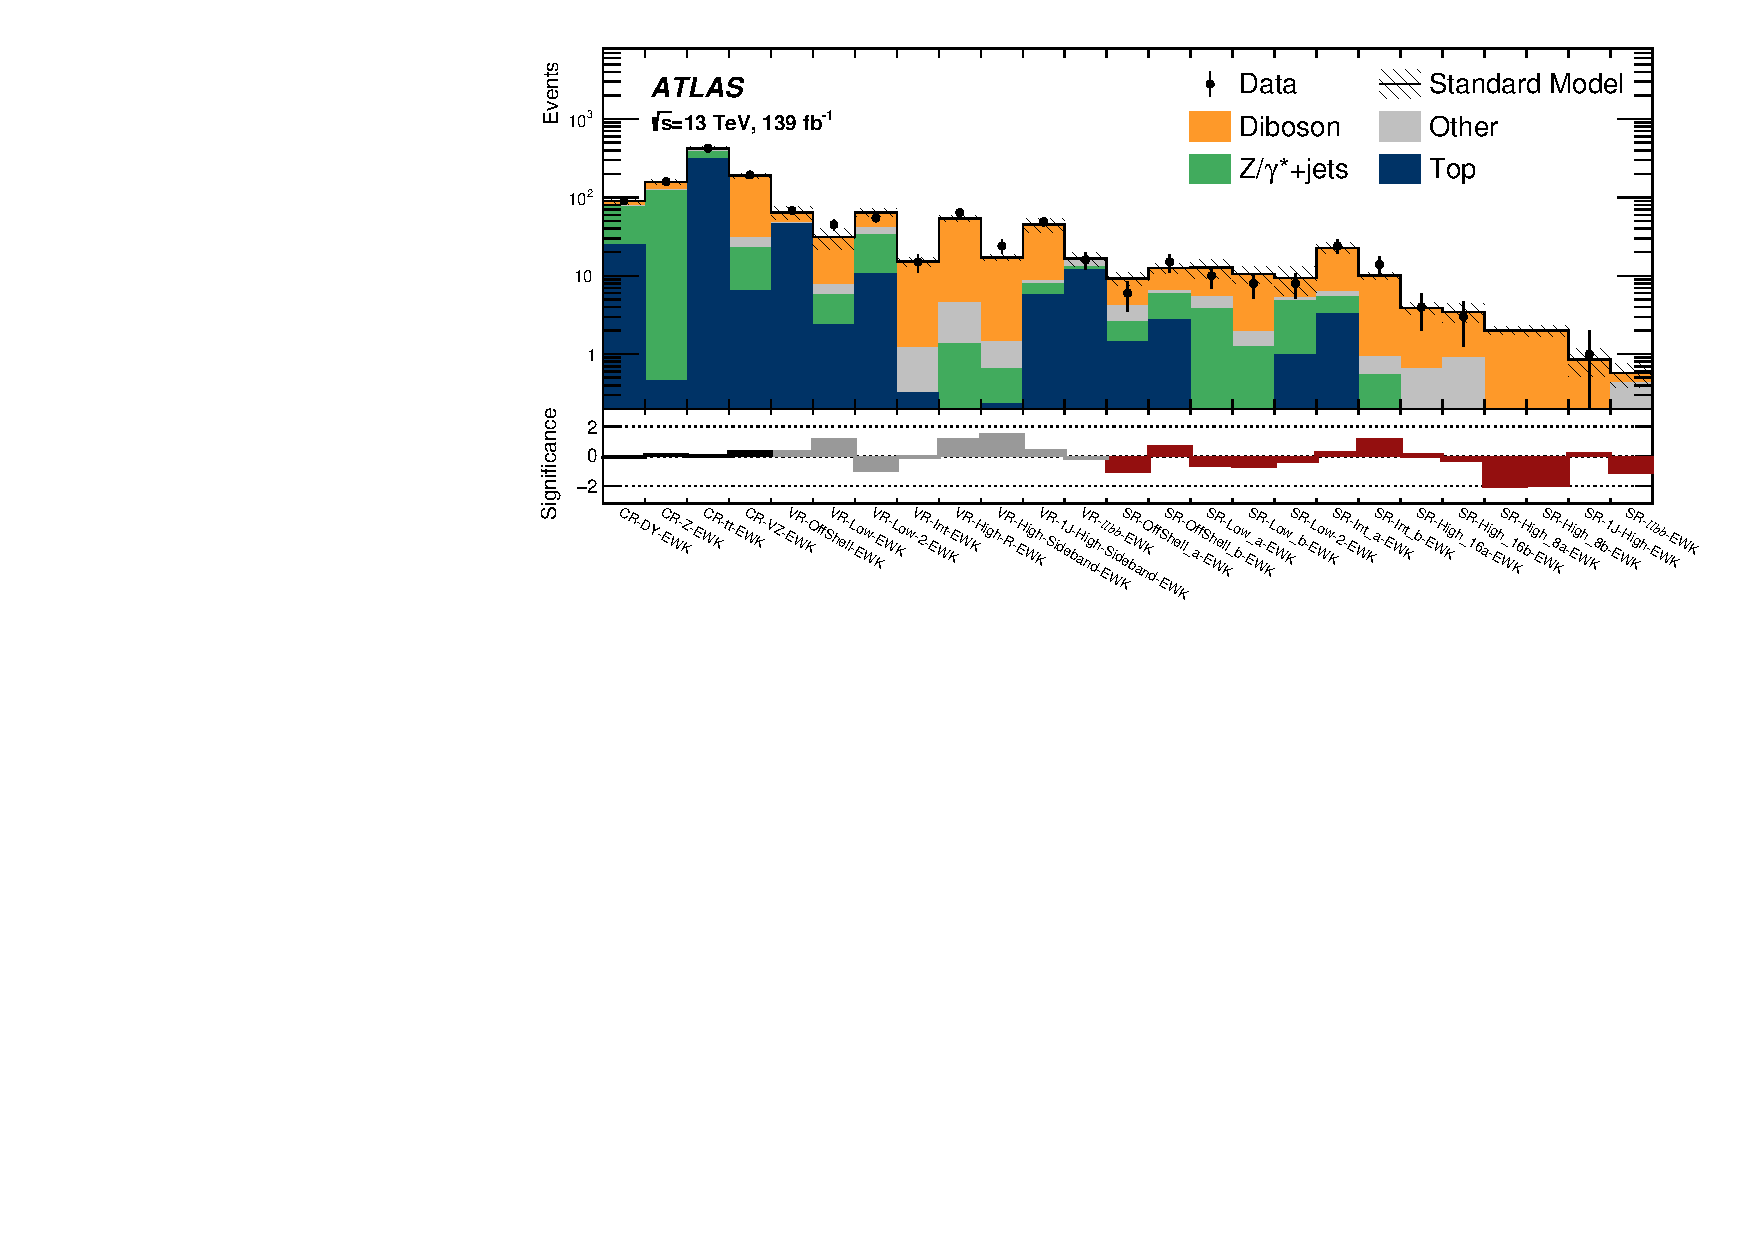
\includegraphics[width=\textwidth]{figures/2ljets_summary_log.pdf}
\caption[
Data of the $\twoljets$-electroweak analysis with \emph{post-fit}
backgrounds
]{%
Data of the $\twoljets$-electroweak analysis with \emph{post-fit}
backgrounds~\cite{atlas2022searches}.
The lower panel shows $S_\mathrm{ATLAS}$ from
Equation~\ref{eqn:significance_atlas}.
Control, validation and signal regions are shown from left to right, with the
regions within each category ordered approximately by their typical $\met$.
Likelihoods from validation regions are not included in the fit.
The `Top' category contains $\ttbar$ and $tW$ processes, and
`Other' contains fake/non-prompt lepton, higgs, triboson, $\ttbar Z$, and other
rare top processes.%
}
\label{fig:2ljets_summary}
\end{figure}

% signal diagrams
\begin{figure}[t]
\centering
\begin{subfigure}{0.48\textwidth}
\centering
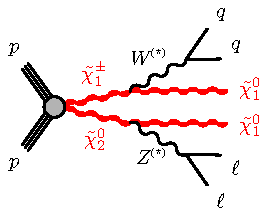
\includegraphics[width=\textwidth]{figures/2ljets_c1n2_llqqn1n1_wz.pdf}
\caption{C1N2}
\end{subfigure}
\hfill
\begin{subfigure}{0.48\textwidth}
\centering
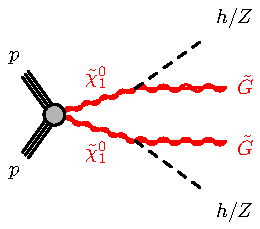
\includegraphics[width=\textwidth]{figures/2ljets_n1n1_hhggzz.pdf}
\caption{GMSB}
\end{subfigure}
\caption[
Supersymmetric signal processes in the $\twoljets$-electroweak analysis
]{%
Supersymmetric signal processes in the $\twoljets$-electroweak analysis.
\emph{Figures are reproduced from the paper%
}~\cite{atlas2022searches, atlas_susy_feynman}.
\\[0.5em]
(a): C1N2, where the initial $\chargino_1\textrm{--}\neutralino_2$ pair
is produced through a $s$-channel $W^{\pm}$ resonance and the masses of
weak bosons in decays are bounded by the mass splitting
$m(\chargino_1, \neutralino_2) - m(\neutralino_1)$.
We explore the parameters
$m(\chargino_1, \neutralino_2)$ and $m(\neutralino_1)$.
\\[0.5em]
(b): GMSB, where the initial $\neutralino_1\textrm{--}\neutralino_1$ pair
is produced by soft decays from pairs including $\chargino_1$,
$\neutralino_2$ or $\neutralino_1$.
Although the $h$ and $Z$ bosons decay to many states, we target
$Z\rightarrow \ell\ell$ with
$h/Z\rightarrow bb/jj$.
We explore the parameters
$m(\neutralino_1)$ and $B(\neutralino_1 \rightarrow h \tilde{G})$ with fixed
$m(\chargino_1, \neutralino_2) - m(\neutralino_1) = 1\,\eV[G]$.
}
\label{fig:2ljets_signal_diagrams}
\end{figure}

% signal region plots
\begin{figure}[tp]
\centering
\begin{subfigure}{0.48\textwidth}
\centering
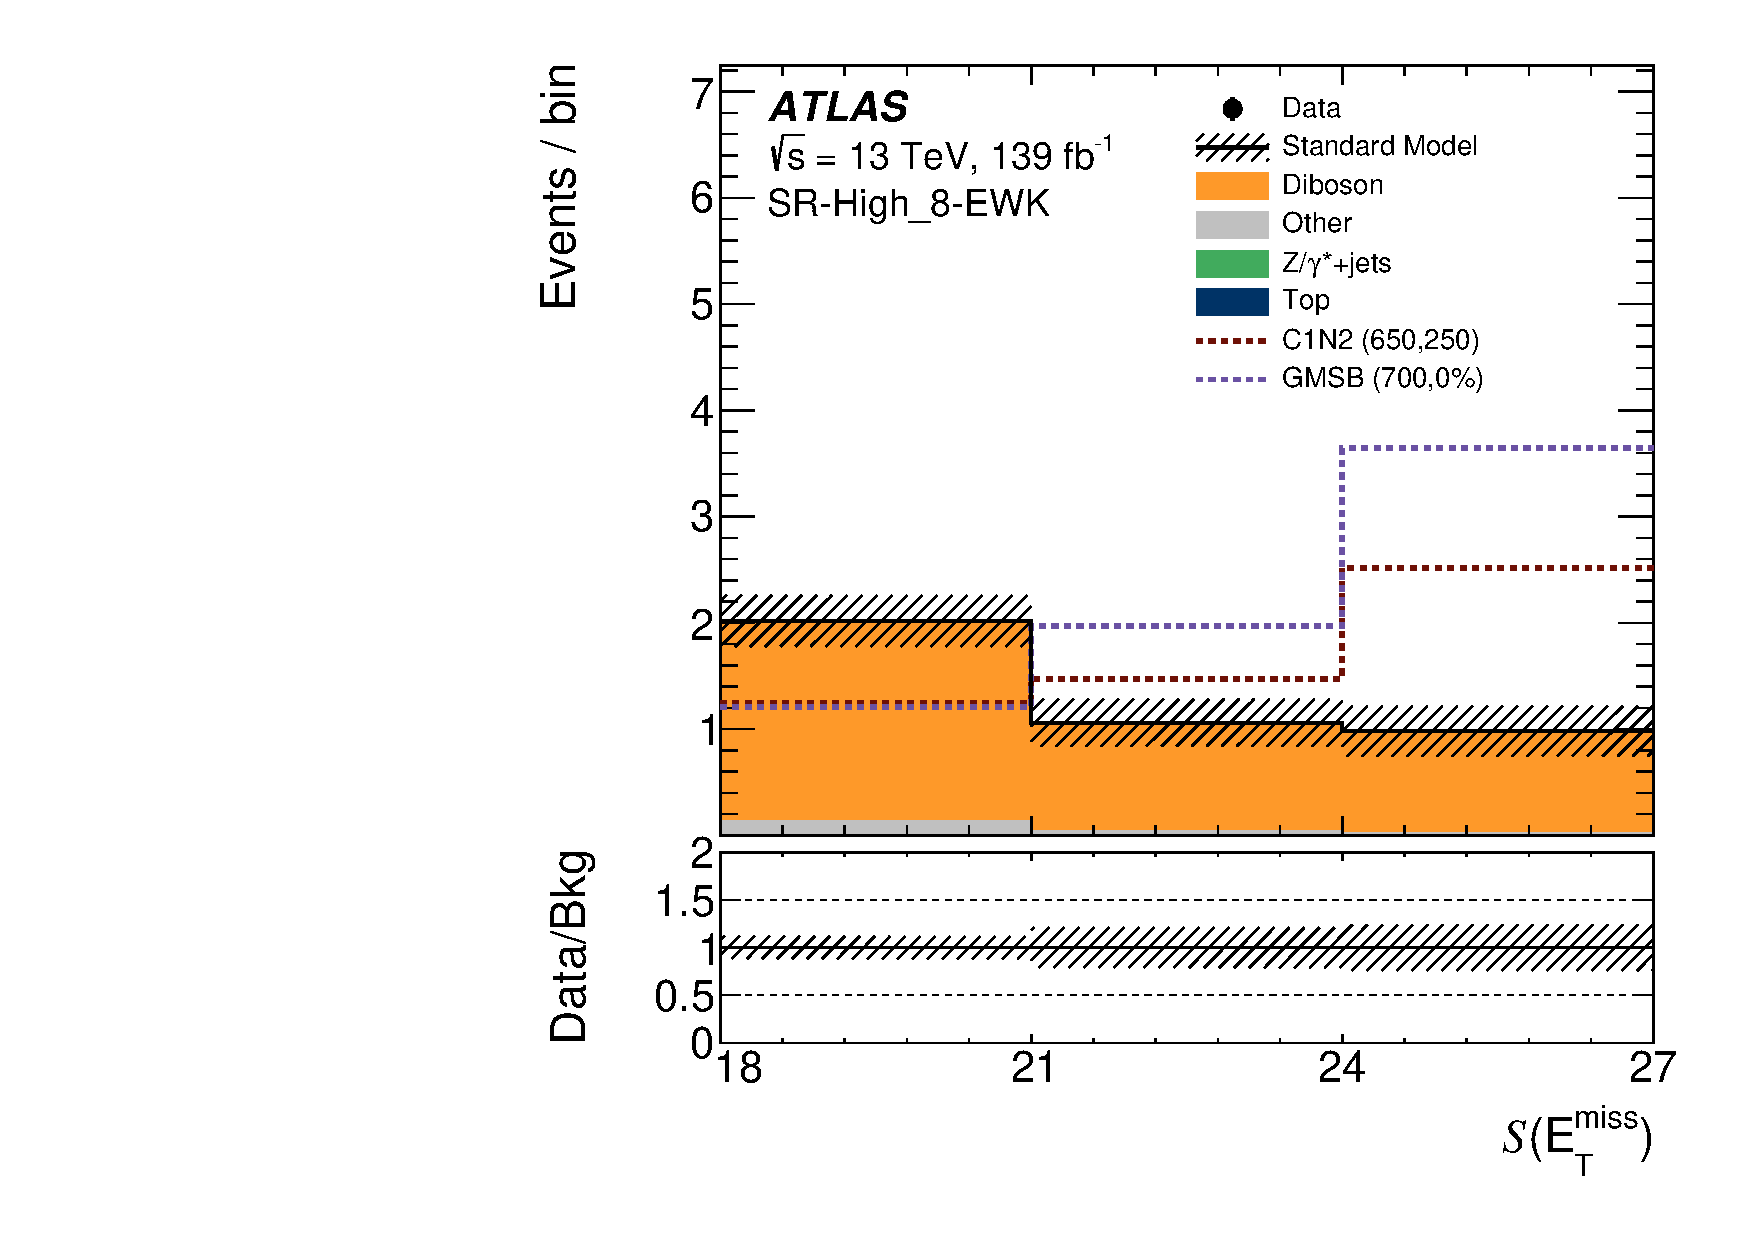
\includegraphics[width=\textwidth]{figures/2ljets_sr_high_8_met_sig.pdf}
\caption{SR-High-8}
\end{subfigure}
\hfill
\begin{subfigure}{0.48\textwidth}
\centering
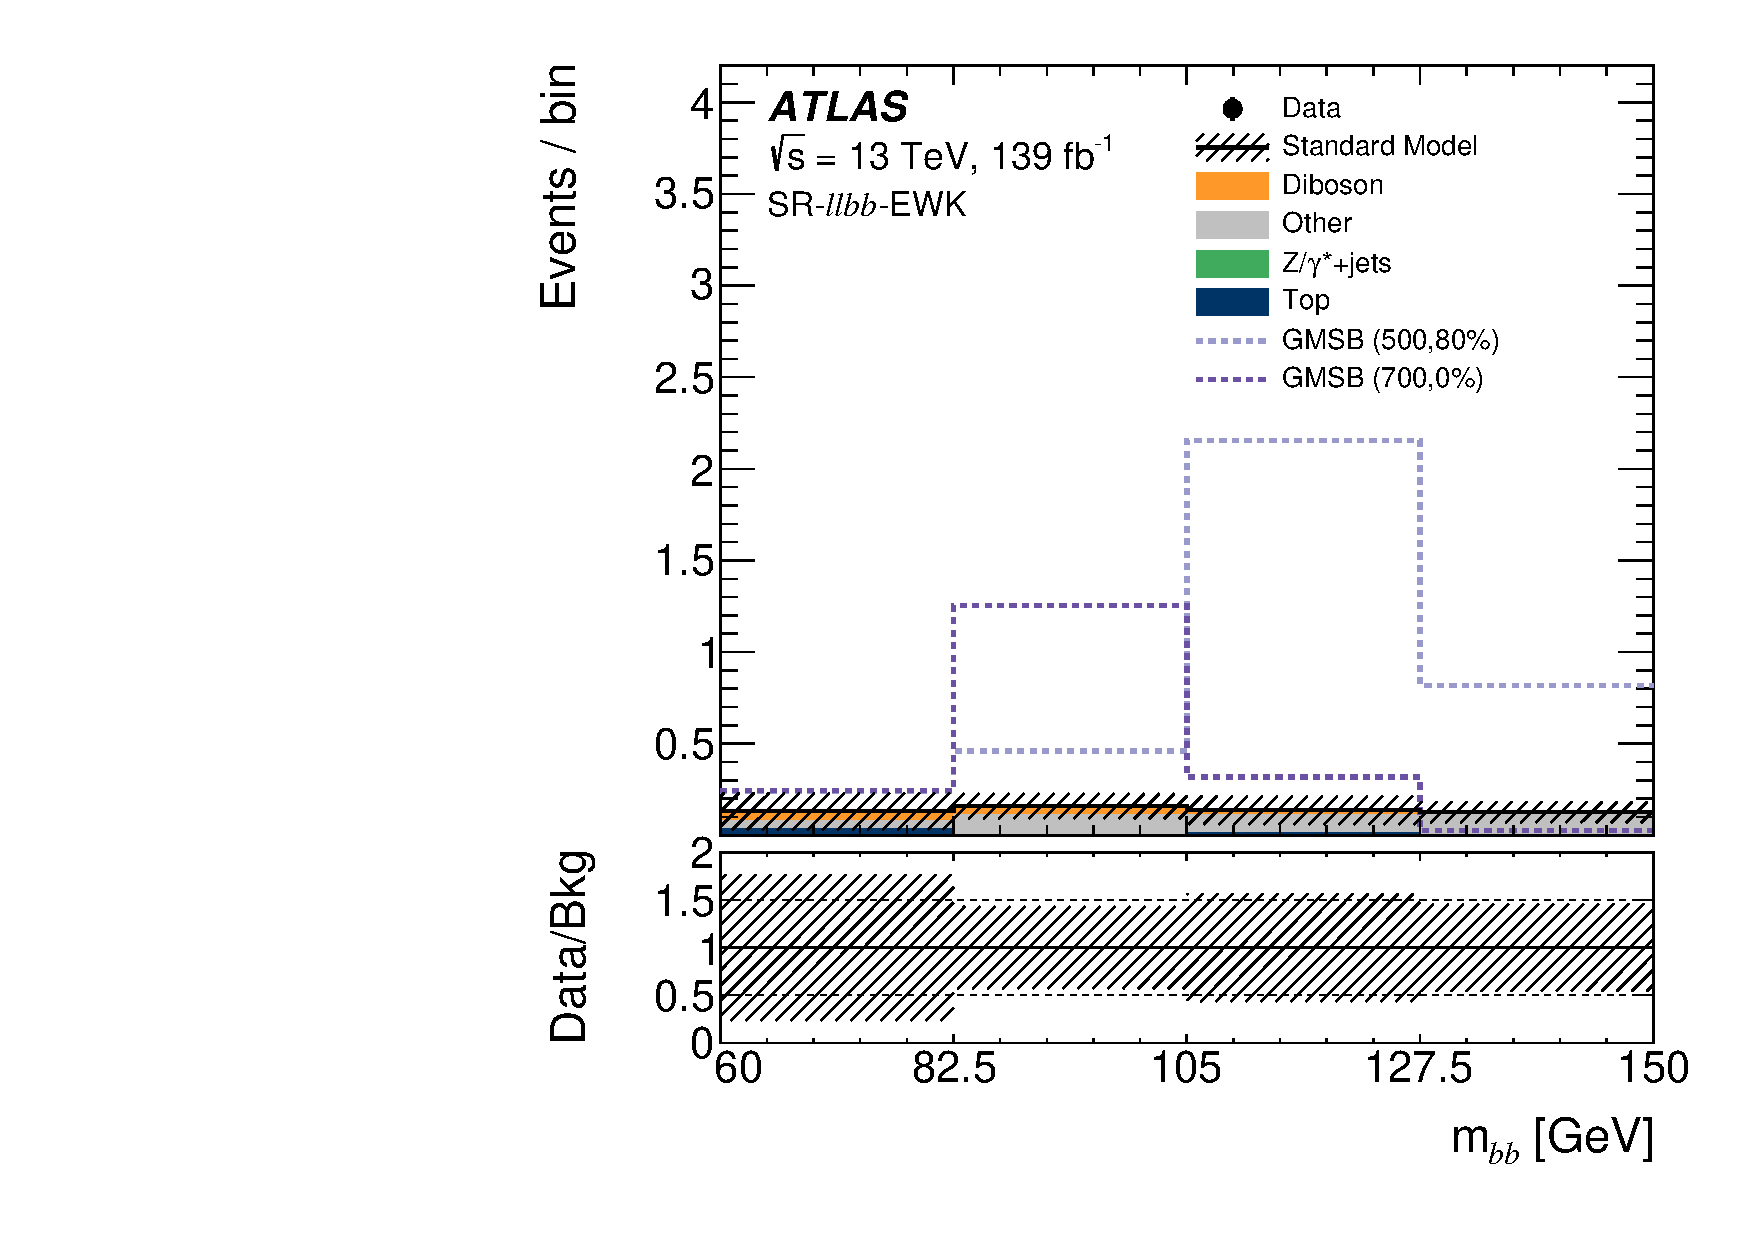
\includegraphics[width=\textwidth]{figures/2ljets_sr_llbb_mbb.pdf}
\caption{SR-$\llbb$}
\end{subfigure}
\\[0.5em]
\begin{subfigure}{0.48\textwidth}
\centering
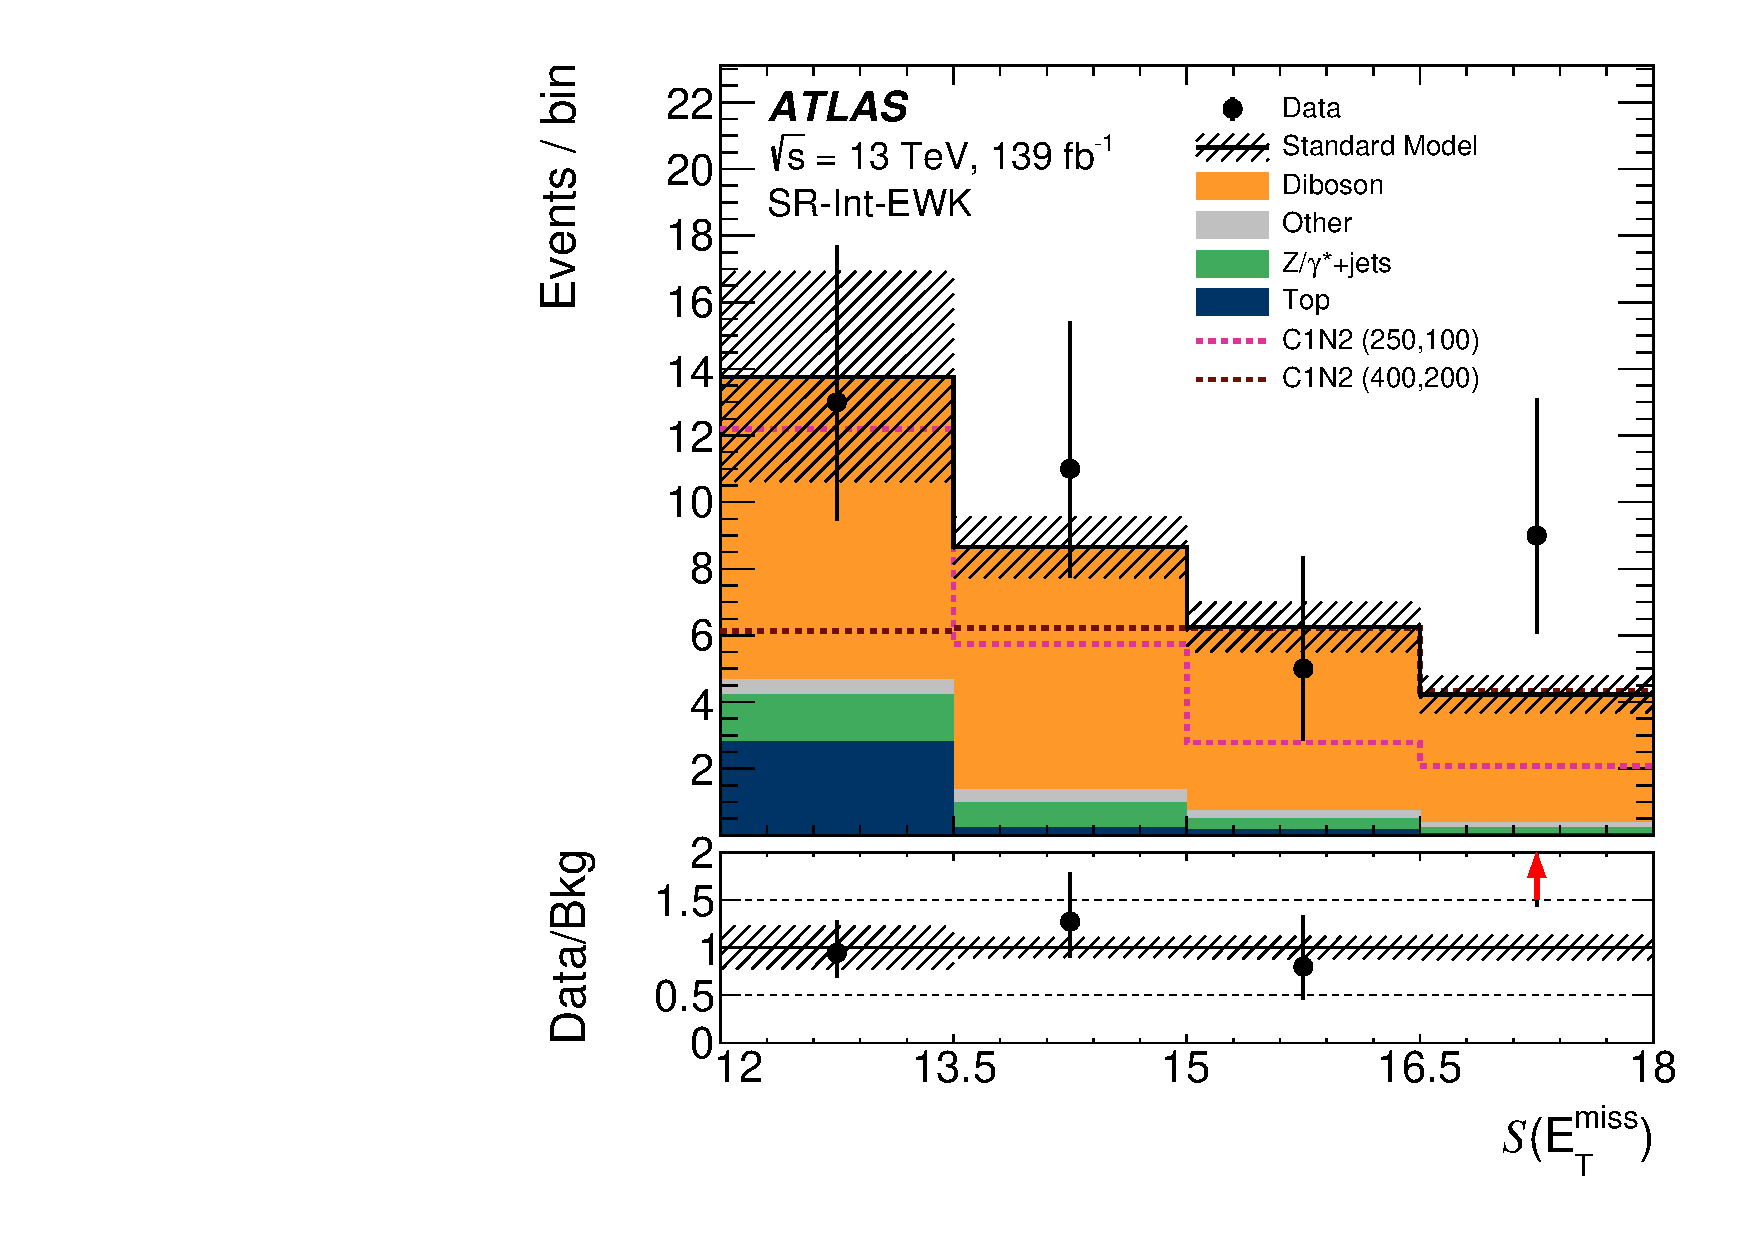
\includegraphics[width=\textwidth]{figures/2ljets_sr_int_met_sig.pdf}
\caption{SR-Int}
\end{subfigure}
\hfill
\begin{subfigure}{0.48\textwidth}
\centering
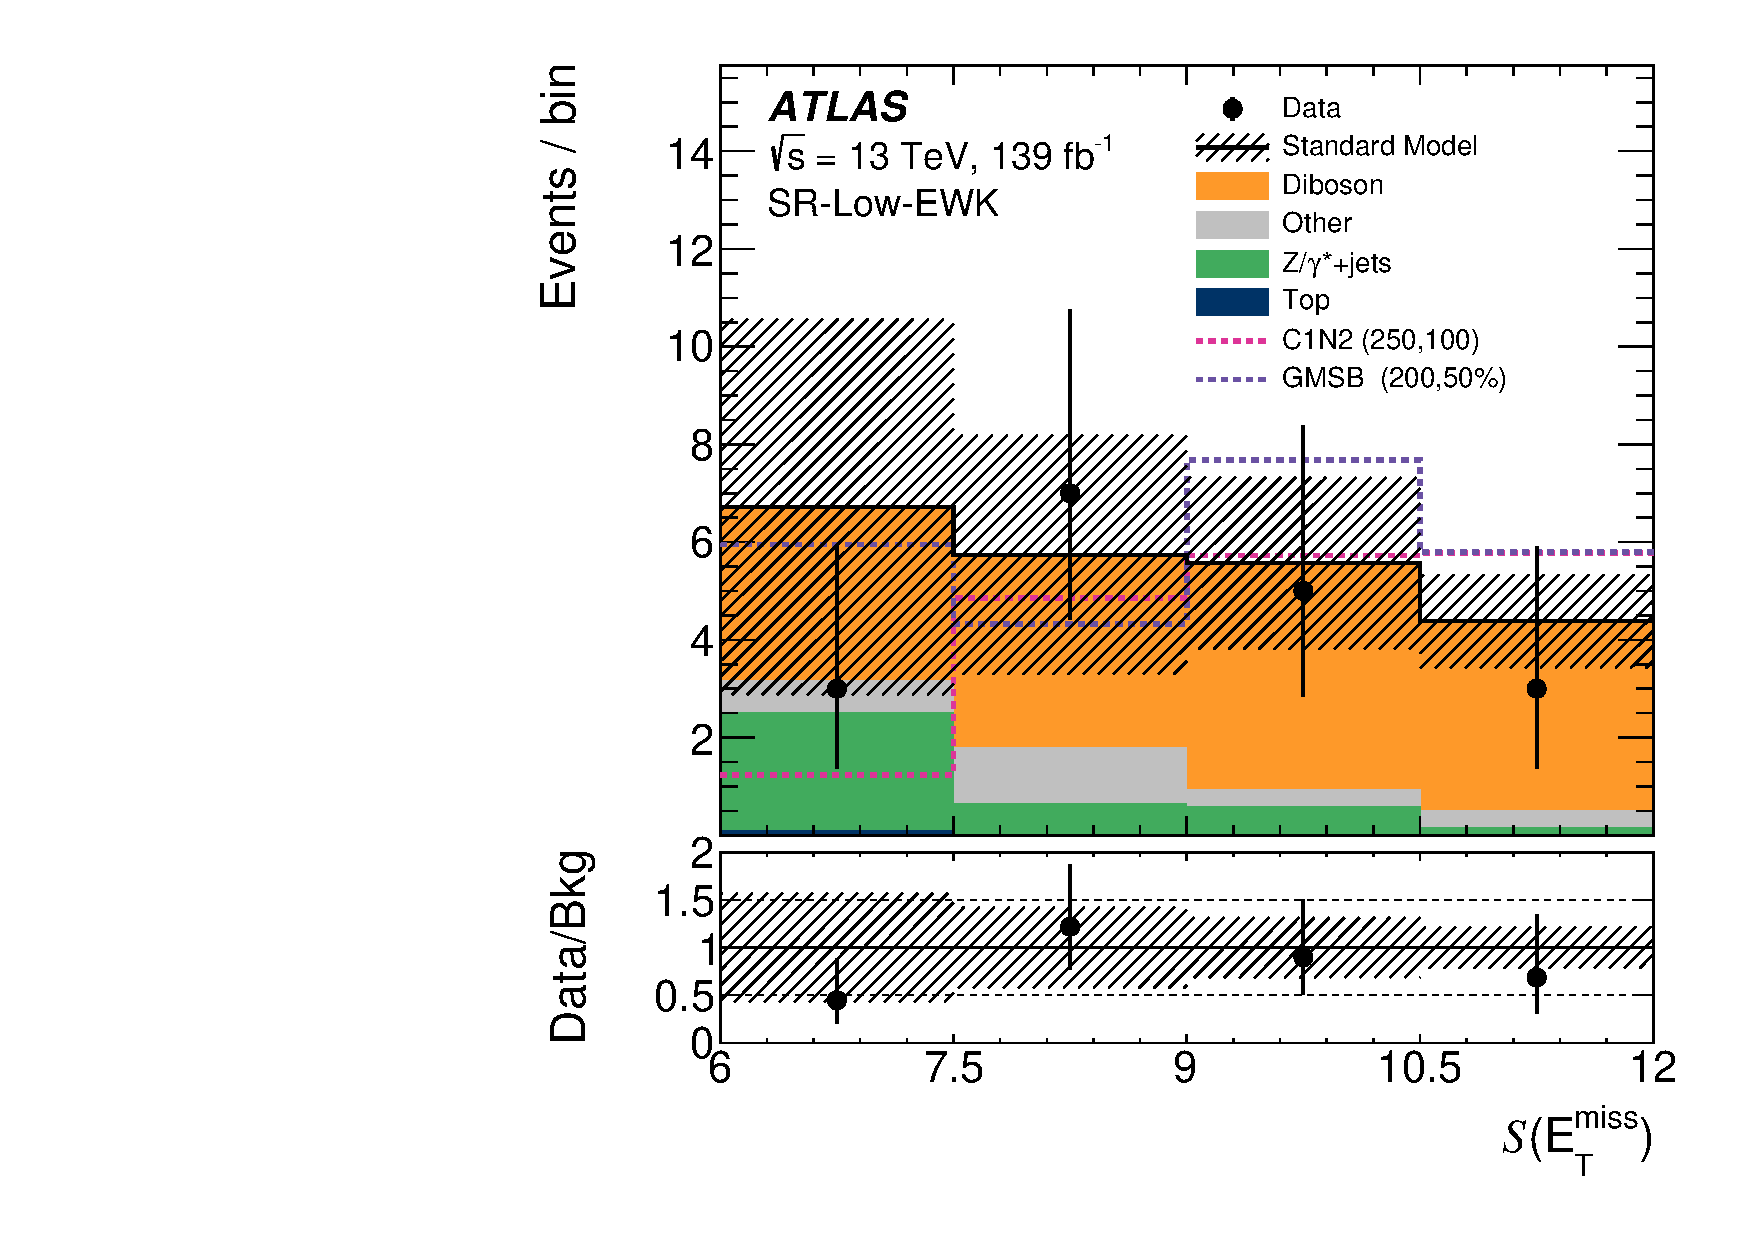
\includegraphics[width=\textwidth]{figures/2ljets_sr_low_met_sig.pdf}
\caption{SR-Low}
\end{subfigure}
\caption[
Example signal region histograms with benchmark signal sample yields overlaid
]{%
Example signal region histograms with benchmark signal sample yields overlaid
as dotted lines~\cite{atlas2022searches}.
Physically, signal yields would add on top of the backgrounds.
Data are shown; regions in the top two plots observe zero data, and
Poisson error bars for $0$ events are hidden for aesthetic reasons.
}
\label{fig:2ljets_signal_examples}
\end{figure}

% exclusion plots
\begin{figure}[tp]
\centering
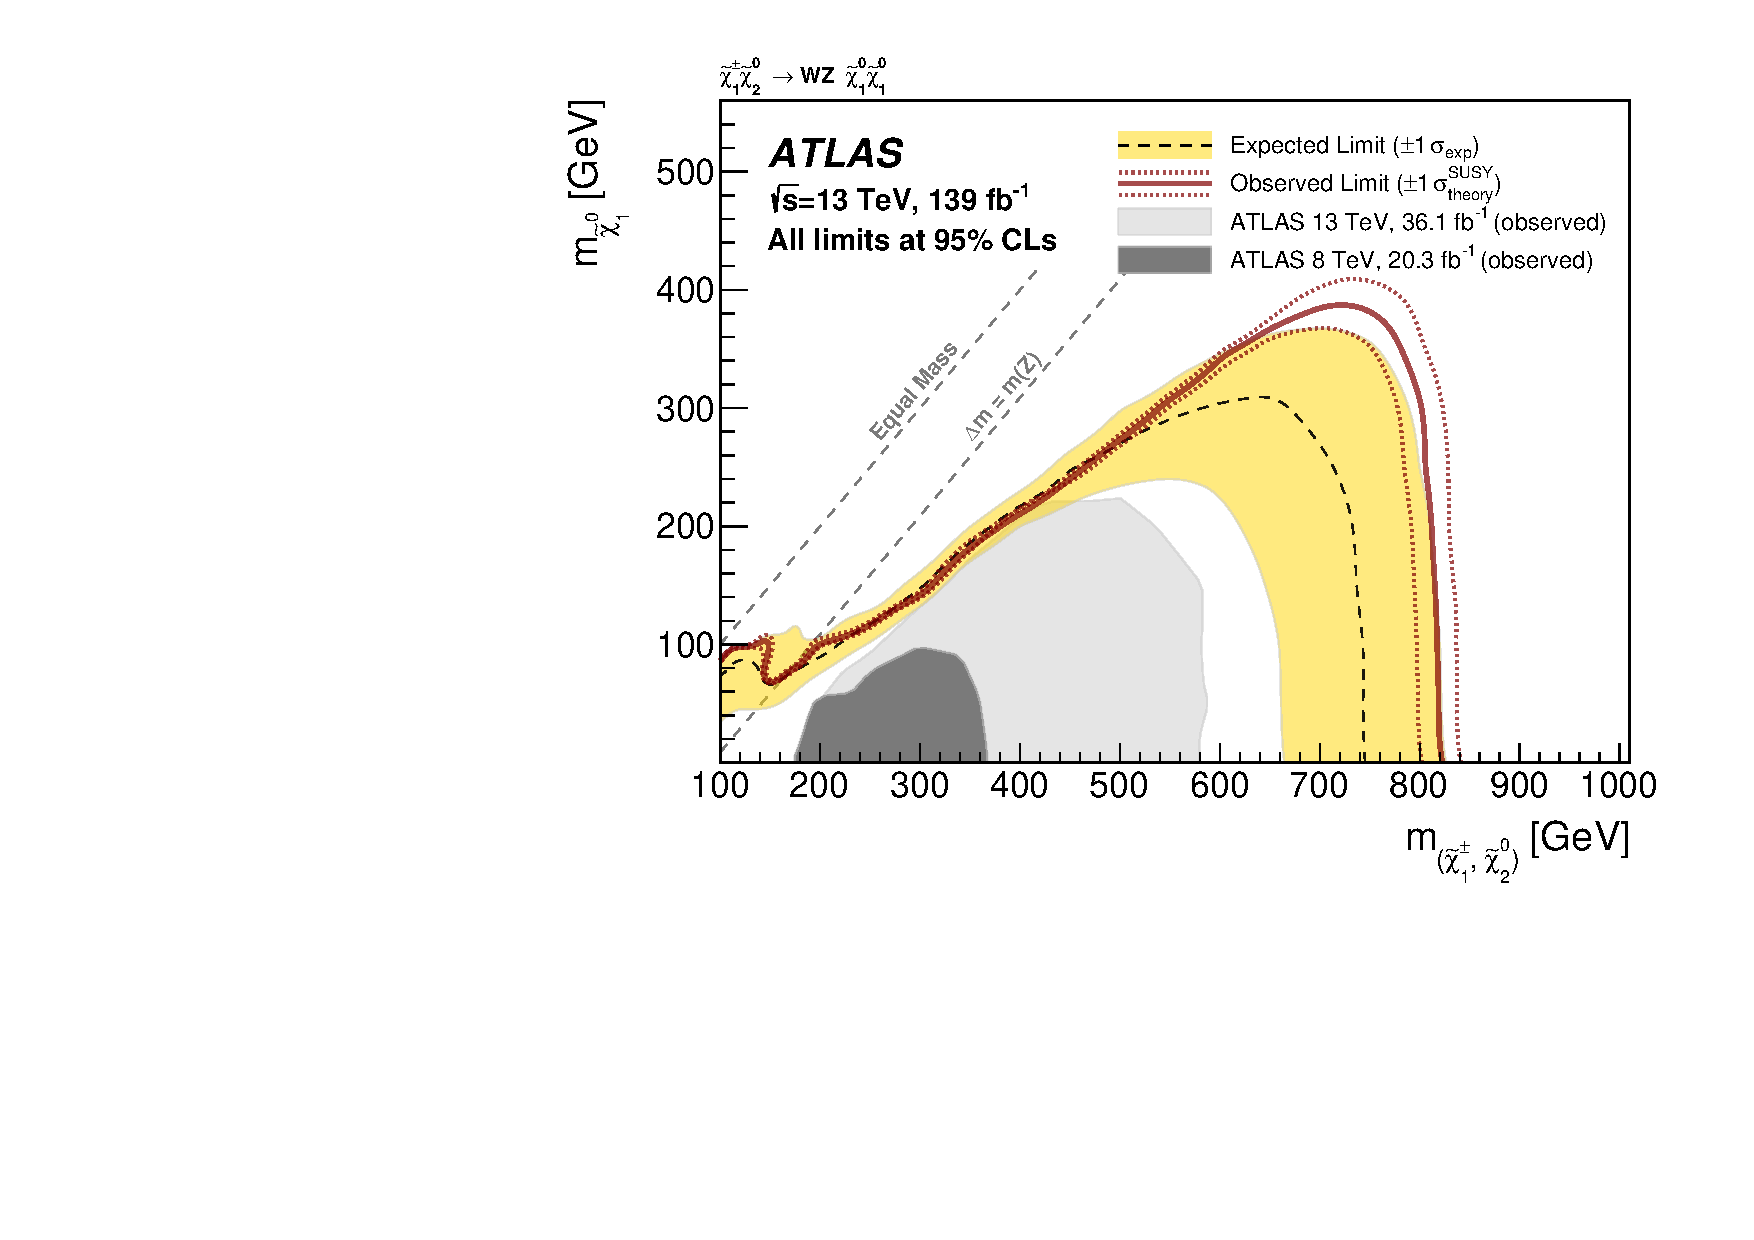
\includegraphics[width=0.99\textwidth]{figures/2ljets_contours_c1n2.pdf}
\caption[
Contours for the C1N2 model in the $\twoljets$-electroweak analysis
]{%
Contours for the C1N2 model in the $\twoljets$-electroweak
analysis~\cite{atlas2022searches}.
\\[0.5em]
Space below the solid red line is labelled as excluded, and its dotted
neighbours show the result if all signal cross-sections are varied up and down
by theoretical error bars.
\\[0.5em]
The yellow band shows the $\pm1$-sigma region of exclusion contours
from asymptotic approximations to the prior distribution of the test statistic.
Grey areas are observed limits from the two-lepton parts
of~\cite{atlas_23l_SUSY_2016_24} and~\cite{atlas_2l_SUSY_2013_11}.
Exclusion is defined by the $95\%$ $\mathrm{CLs}$ prescription
in asymptotic approximations.
All contours are interpolated from a sparse grid.
}
\label{fig:2ljets_contours_c1n2}
\end{figure}

\begin{figure}[tp]
\centering
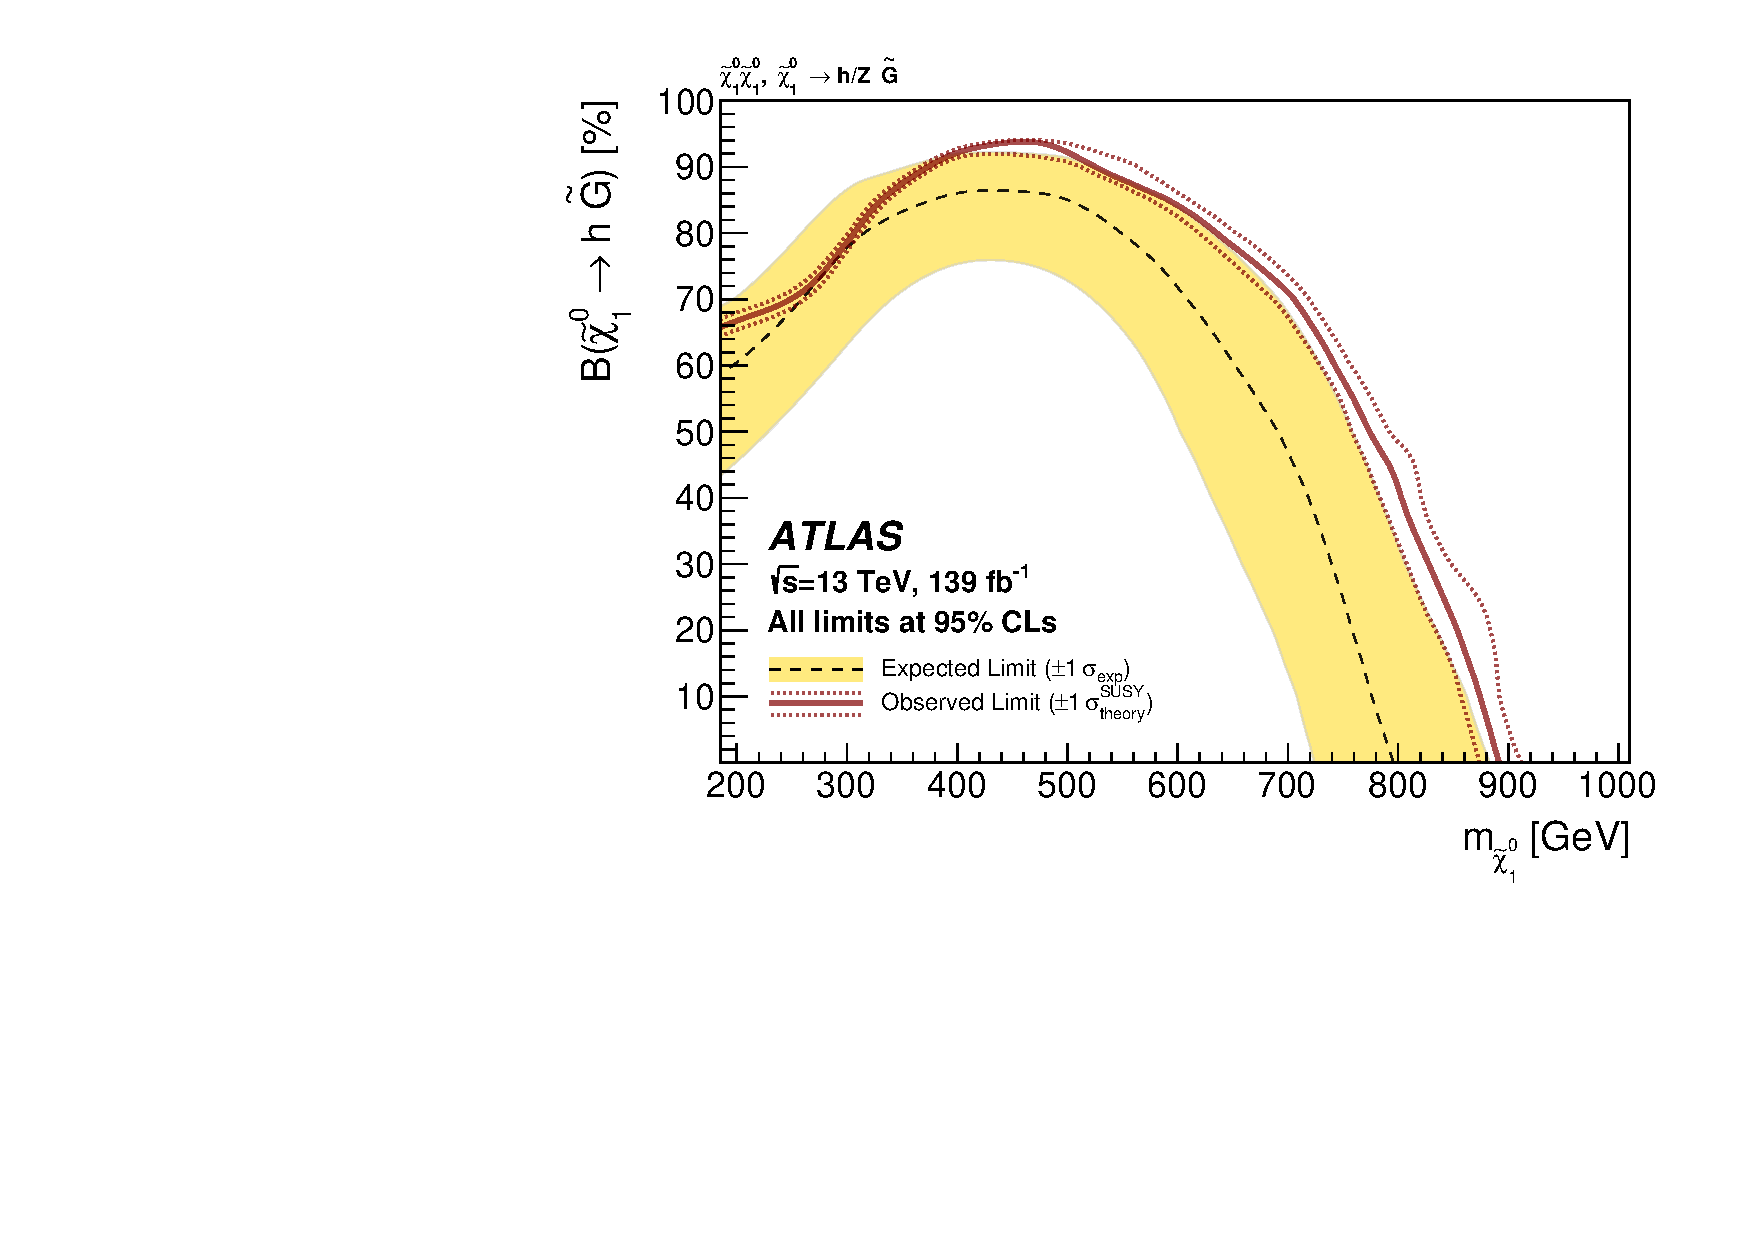
\includegraphics[width=0.99\textwidth]{figures/2ljets_contours_gmsb.pdf}
\caption[
Contours for the GMSB model in the $\twoljets$-electroweak analysis
]{%
Contours for the GMSB model in the $\twoljets$-electroweak
analysis~\cite{atlas2022searches}.
\\[0.5em]
Space below the solid red line is labelled as excluded, and its dotted
neighbours show the result if all signal cross-sections are varied up and down
by theoretical error bars.
\\[0.5em]
The yellow band shows the $\pm1$-sigma region of exclusion contours
from asymptotic approximations to the prior distribution of the test statistic.
Exclusion is defined by the $95\%$ $\mathrm{CLs}$ prescription
in asymptotic approximations.
All contours are interpolated from a sparse grid.
}
\label{fig:2ljets_contours_gmsb}
\end{figure}

% upper limits
% definitely want this after pictures
\FloatBarrier
\begin{table}[tp]
\centering
% custom separator for aligned +-
% https://stackoverflow.com/a/2132998
\begin{tabular*}{\textwidth}{lr@{$~\pm~$}lcccccc}
& \multicolumn{2}{c}{Fitted}
& Data
& $A\epsilon\sigma_{\mathrm{obs}}^{95}~\mathrm{fb}$
& $S_{\mathrm{obs}}^{95}$
& $S_{\mathrm{exp}}^{95}$
& $\mathrm{CLb}$
& $p_{s\!=\!0}$
\\[1.5ex]
DR-OffShell & $22.1$ & $2.7$ & $21$ & $0.10$ & $14.3$ & $12.3^{+4.7}_{-3.1}$ & $0.68$ & $0.50$
\\[.5ex]
DR-Low & $22$ & $4$ & $18$ & $0.08$ & $10.8$ & $15.3^{+5.7}_{-4.0}$ & $0.09$ & $0.50$
\\[.5ex]
DR-Int & $35$ & $4$ & $38$ & $0.15$ & $20.9$ & $17.5^{+5.9}_{-3.9}$ & $0.73$ & $0.23$
\\[.5ex]
DR-High & $3.9$ & $0.5$ & $0$ & $0.02$ & $3.0$ & $5.6^{+2.2}_{-1.5}$ & $0$ & $0.50$
\\[.5ex]
DR-$\llbb$ & $0.51$ & $0.20$ & $0$ & $0.02$ & $3.0$ & $3.0^{+1.3}_{-0.0}$ & $0.19$ & $0.50$
\\[.5ex]
\end{tabular*}
\caption[
Upper limit results in $\twoljets$-electroweak discovery regions
]{%
Upper limit results in $\twoljets$-electroweak discovery
regions~\cite{atlas2022searches}.
The fitted yield is in the background-only model constrained by the data in each region.
Limits are intended to reflect constrains on additive signal contributions.
\\[0.5em]
Left to right:
the region name,
the post-fit background expectation,
the number of data observed,
the observed $95\%$ $\mathrm{CLs}$ upper limit on the visible cross-section
$\langle\epsilon\sigma\rangle_\mathrm{obs}^{95}$,
its corresponding signal expectation $S_\mathrm{obs}^{95}$,
the expected $95\%$ upper limits on the signal expectation $S_\mathrm{exp}^{95}$
as would be obtained were the test statistic given by its central or
$\pm1$-sigma variations,
$\mathrm{CLb}$ evaluated with the signal expectation set to the observed upper limit,
and the discovery $p$-value (capped at $0.5$) with its equivalent significance.
\\[0.5em]
Upper limits use the one-sided profile likelihood test statistic.
The discovery $p$-value uses a profile likelihood test statistic in a one-sided test.
All $p$-values are estimated by simulation of alternative data.
\\
\TODO{add labels and references to asymptotic formulae paper}
\\
\TODO{reference pdg rounding}
}
\label{tab:2ljets_discovery}
\end{table}

\FloatBarrier
\subsection{Contributions}

In this subsection, I claim attributions of work on the $\twoljets$ analysis
and related \atlas\ efforts.

\begin{itemize}
\item Design, implementation, and execution of the electroweak part of the analysis.
\item Service as `analysis contact' from January to October 2020.
\item Production of main data inputs for all three $\twoljets$ analyses
and the RJR $3\ell$ search~\cite{atlas_rjr_3l_SUSY_2019_09},
Production of all systematic variations for the background samples;
other group members assisted with the central background sample.
Production of all electroweak signal samples and their systematic variations.
\item \TODO{?Evaluation of Monte Carlo $Z$+jets uncertainties for RJR signal regions
which indicated they exceeded $100\%$}
\item \TODO{Various collaborations with group members on scripts to conduct
tasks which were common between the searches.}
\item Integration of the electroweak analysis with ATLAS combinations and
pMSSM scan efforts, by performing their validation studies and serializing the
analysis results.
\item Preparation of electroweak results for publication in the
paper~\cite{atlas2022searches} and the public HEPData
record~\cite{maguire2017hepdata}.
\end{itemize}
Except where specified, I produced all figures presented in this thesis.
Many plotting scripts, however, are modified from versions inherited from
many \atlas\ members past and present, to whom I am grateful.

Of the large collaboration involved in this project, a great deal of credit is
due to the following colleagues, labelled with their primary focus within
the $\twoljets$ search effort:
Knut Oddvar Vadla (electroweak),
Sarah Williams (electroweak),
Jason Lea Oliver (RJR),
Abhishek Sharma (RJR),
Jonathan Long (strong),
Arka Santra (strong),
Matt Zhang (strong),
Yumeng Cao (various),
Eirik Gramstad (fake/non-prompt leptons),
Benjamin Henry Hooberman (leadership).
Cheers.

\clearpage
\FloatBarrier
\section{Summaries}
\label{sec:2ljets_context}
% previous results on 2(/3)L from ATLAS
% other constraints on these models from ATLAS/CMS
% previous region design, motivation for this work
Previous analyses of \atlas\ data have explored similar selections of
two leptons, jets, and missing transverse momentum.
Quite a few analyses, in fact.
This project exists to supplement those results with information from the full
LHC Run~2 data-set, which was completed in 2018 and contains
$139~\mathrm{fb}^{-1}$ of usable proton-proton collisions at
$\sqrt{s} = 13\,\eV[T]$.
Leverage of the increased data quantity is one key aim.
Analysis quality also might be improved if our designs can take lessons from
the experiences of previous work.

% electroweak
% Run 1 data~\cite{atlas_2l_SUSY_2013_11},
% partial Run~2 data~\cite{atlas_23l_SUSY_2016_24},
% atlas_rjr_23l_SUSY_2017_03,
% atlas_rjr_mimic_SUSY_2018_06
The $\twoljets$ analysis is a trinity,
of which all three parts update previously published \atlas\ results.
These three parts are named `RJR', `electroweak', and `strong', each of which
is described in its historical context in this section.

Recursive Jigsaw Reconstruction (RJR) is an algorithm for constructing useful
event variables.
The $\twoljets$-RJR analysis, detailed in Section~\ref{sec:2ljets_origins_rjr},
uses RJR variables to define its regions in a signal-independent search.

The $\twoljets$-strong analysis is
detailed in Section~\ref{sec:2ljets_origins_strong} and
searches for effects from the strong sector.
It also uses conventional event variables, and focuses on features in the
distribution of the invariant masses of lepton pairs.

My primary contributions are to the $\twoljets$-electroweak analysis,
detailed in Section~\ref{sec:2ljets_origins_electroweak},
which uses conventional (non-RJR) event variables to define a collection of
orthogonal regions, and performs a search for effects from the electroweak
sectors of supersymmetric models.

\FloatBarrier
\subsection{RJR}
\label{sec:2ljets_origins_rjr}

\begin{figure}[tp]
\centering
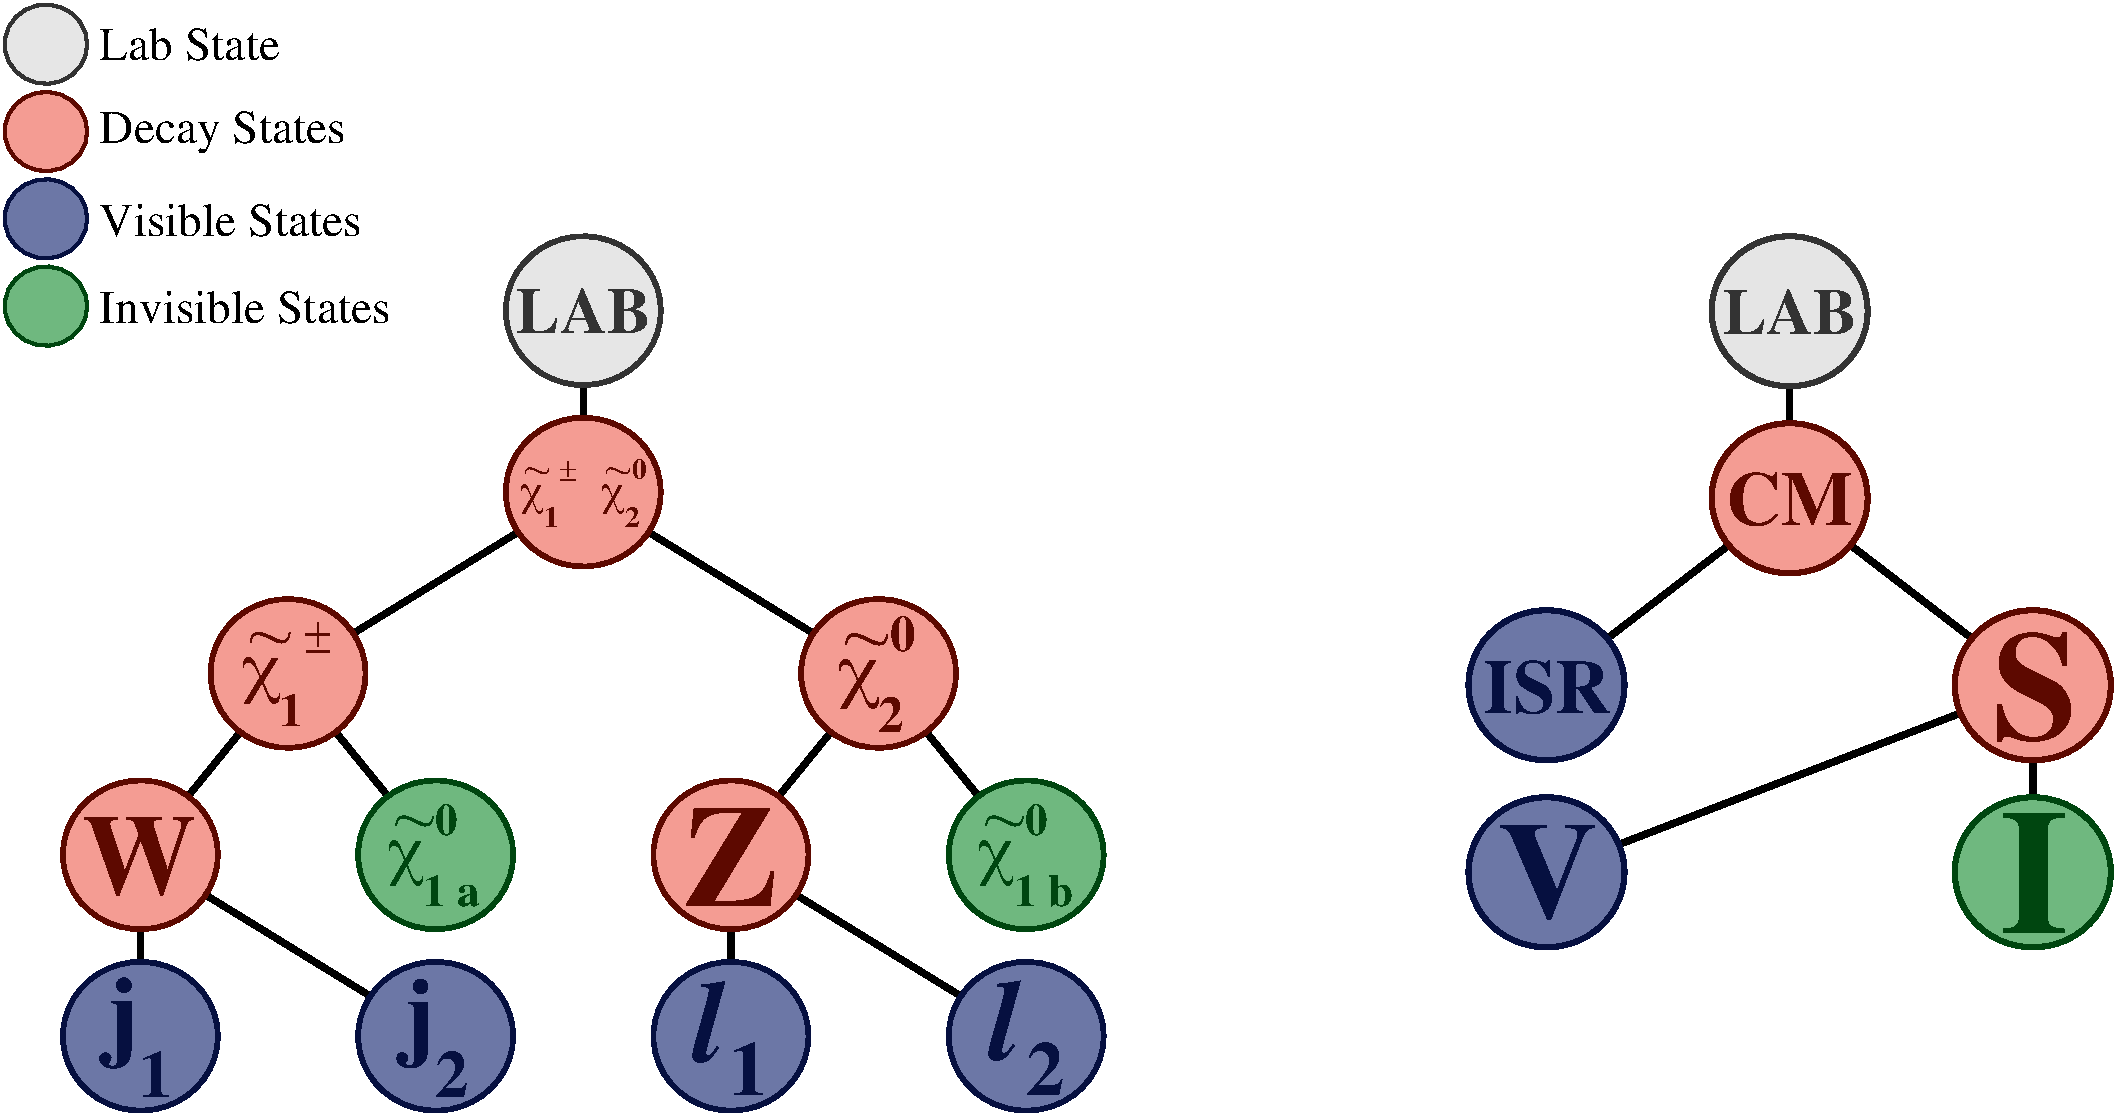
\includegraphics[width=0.9\textwidth]{figures/2ljets_rjr_trees.pdf}
\caption[
Decay trees for the $\twoljets$-RJR analysis
]{%
Decay trees for the $\twoljets$-RJR analysis.
\emph{This figure was made by the RJR team.}~\cite{atlas2022searches}.
Both diagrams represent processes which are targetted in the electroweak
analysis.
(left) A fully-resolved decay tree with its particles labelled.
(right) Only the $Z\rightarrow\ell\ell$ \underline{V}ector boson)
is resolved, but the supersymmetric system recoils off
hard QCD jets labelled ``ISR'', boosting the \underline{I}nvisible particles,
to generate visibly large $\met$ in models with small mass-splittings.
The same approach is used for SR-OffShell selections in the electroweak
analysis.
}
\label{fig:2ljets_rjr_decay_trees}
\end{figure}

The Recursive Jigsaw Reconstruction (RJR) method interprets reconstructed
particle data by reconciling them with user-specified decay trees, and works
by making decisions of how to assign four-momenta to different `systems',
which are nodes of the chosen the decay graph.
Event variables are then evaluated in those systems' rest
frames~\cite{jackson2017sparticles, jackson2017rjr}.

In this way, RJR variables get some intelligence in how parent particles are
reconstructed from their visible decay products, as well as approximate
independence from uninteresting boosts, particularly those from the emission of
QCD jets outside the supersymmetric decay tree.

Over the last several years, RJR event variables have been demonstrated to be
effective for interpreting supersymmetric particle physics
data~\cite{santoni2018probing},
and have been used in numerous \atlas\ searches~\cite{%
atlas_rjr_SUSY_2016_07,
atlas_rjr_SUSY_2016_15,
atlas_rjr_SUSY_2016_16,
atlas_rjr_23l_SUSY_2017_03,
atlas_rjr_SUSY_2018_12,
atlas_rjr_EXOT_2019_19,
atlas_rjr_3l_SUSY_2019_09
}.
They have also influenced the designs of other analyses which do not use
RJR variables themselves~\cite{atlas_rjr_mimic_SUSY_2018_06}.

Two decay trees are used in the $\twoljets$-RJR analysis, with signal region
each.
These trees target C1N2-like scenarios similar to those also considered in the
$\twoljets$-electroweak search,
and illustrated in Figure~\ref{fig:2ljets_rjr_decay_trees}.

\subsubsection{Former excesses}
Excess data were observed in several signal regions of the partial Run~2
search ``for chargino-neutralino production using recursive
jigsaw reconstruction in final states with two or three charged
leptons''~\cite{atlas_rjr_23l_SUSY_2017_03},
which used $36.1~\mathrm{fb}^{-1}$ of proton-proton collisions at
$\sqrt{s} = 13\,\eV[T]$.
That search reported notable excesses in four signal regions.
Of these, two required two charged leptons
($\mathrm{SR}2\ell\_\mathrm{Low}$ and $\mathrm{SR}2\ell\_\mathrm{ISR}$),
and the other two required three
($\mathrm{SR}3\ell\_\mathrm{Low}$ and $\mathrm{SR}3\ell\_\mathrm{ISR}$).

Although the largest local excess was reported as ``$3.0$ standard deviations'',
which is not particularly large, the pattern of four related regions with
excess data can understandably draw attention.

Both $\mathrm{SR}3\ell\_\mathrm{Low}$ and $\mathrm{SR}3\ell\_\mathrm{ISR}$
have been revisited with the full Run~2 data-set and updated background
modelling;
the update sees ``no significant excesses''~\cite{atlas_rjr_3l_SUSY_2019_09}.
These regions have also been approximated without direct use of RJR event
variables;
those approximations also find data ``in agreement'' with the background
model~\cite{atlas_rjr_mimic_SUSY_2018_06}.

The $\twoljets$-RJR serves to analysis reproduce
$\mathrm{SR}2\ell\_\mathrm{Low}$ and $\mathrm{SR}2\ell\_\mathrm{ISR}$,
with the full Run~2 data-set and updated background modelling,
and asks whether the excesses persist.
They do not.

Summary plots for $\twoljets$-RJR and the former 2 and 3 lepton analysis,
including these signal regions with former excesses,
are displayed in Figure~\ref{fig:2ljets_rjr_summaries}.

\begin{figure}[tp]
\centering
\begin{subfigure}{0.48\textwidth}
\centering
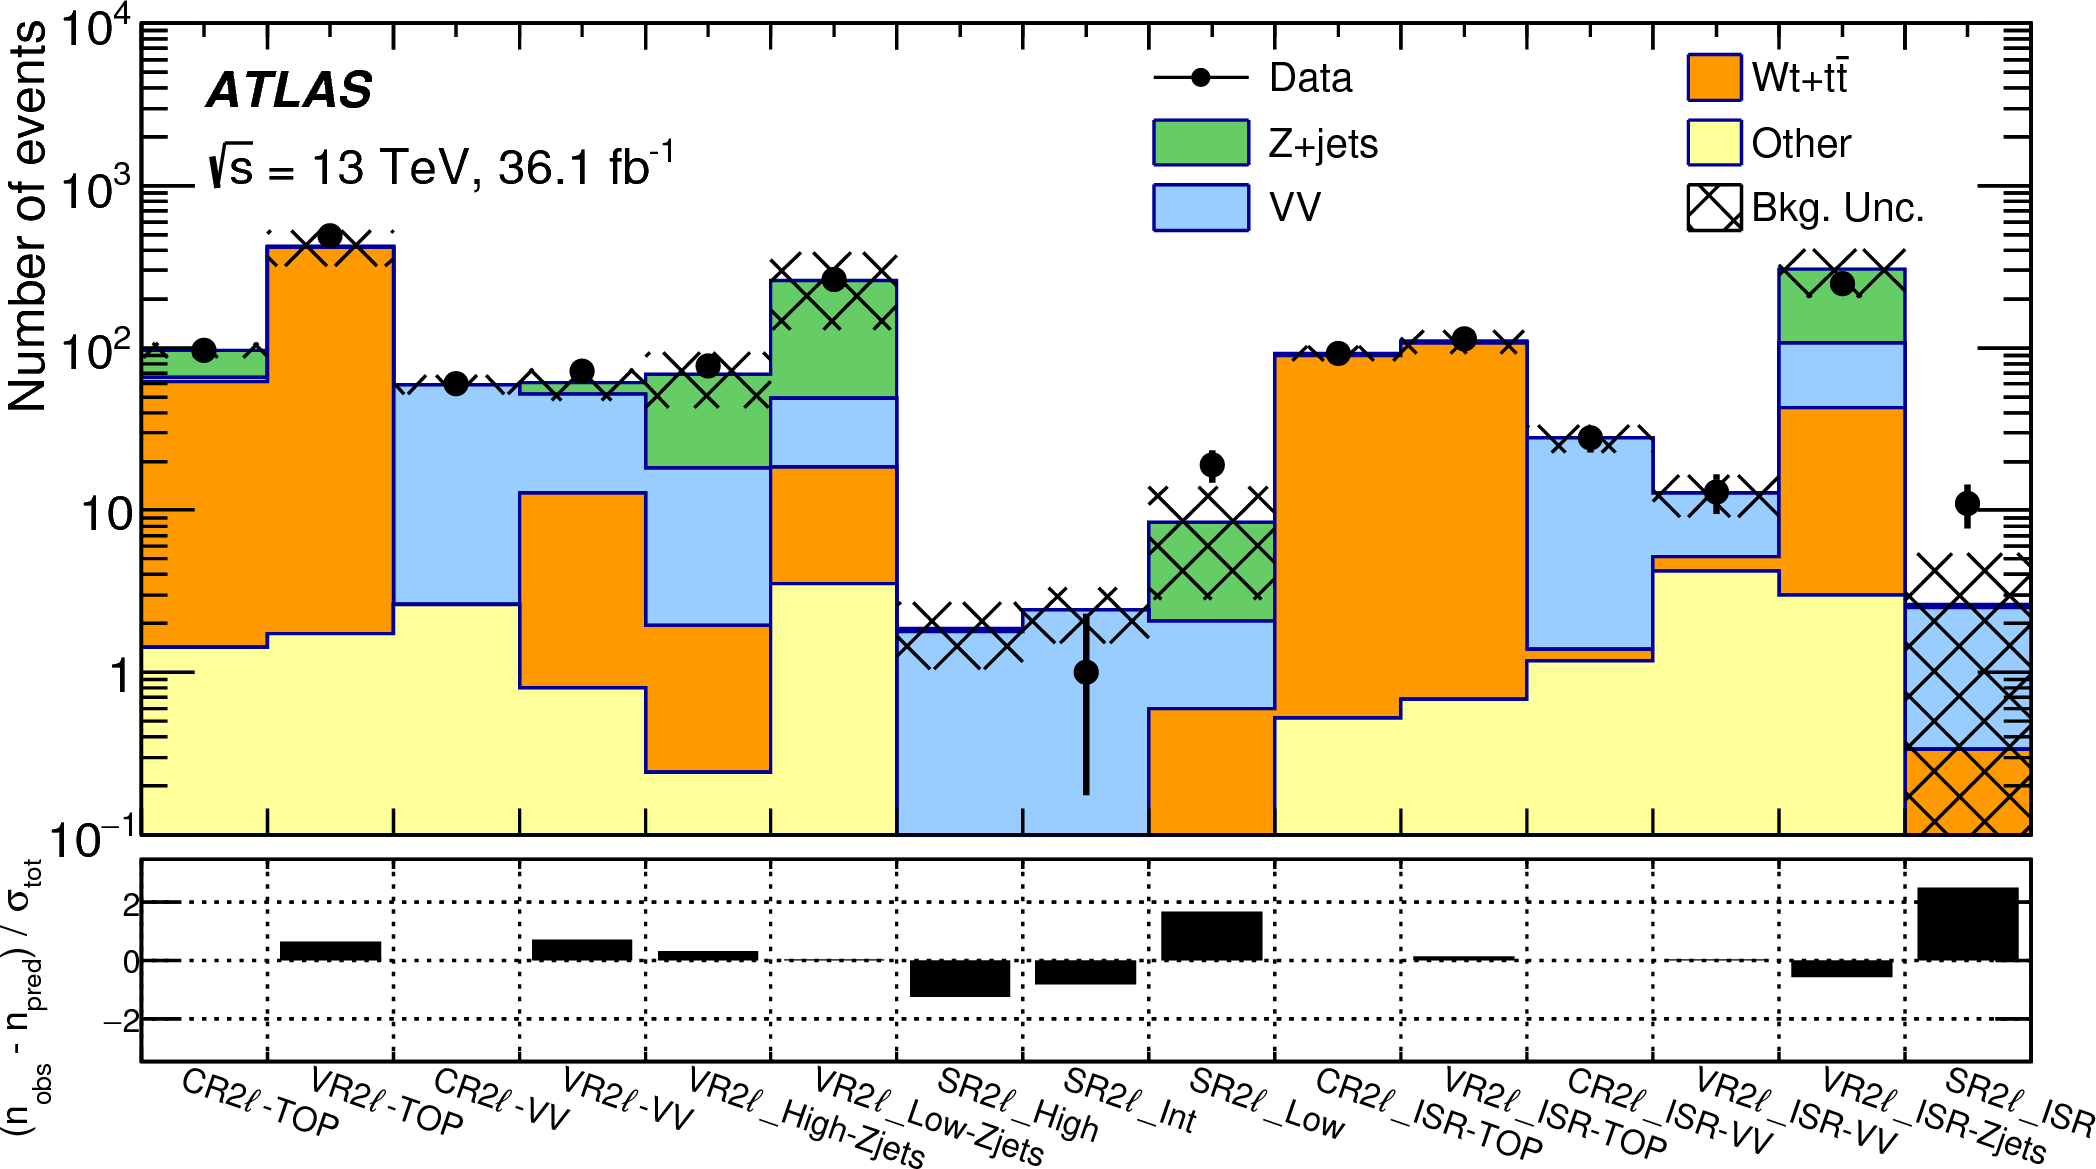
\includegraphics[width=\textwidth]{figures/2ljets_rjr_23l_2l_summary.png}
\caption{$2\ell$ RJR~\cite{atlas_rjr_23l_SUSY_2017_03}}
\end{subfigure}
\hfill
\begin{subfigure}{0.48\textwidth}
\centering
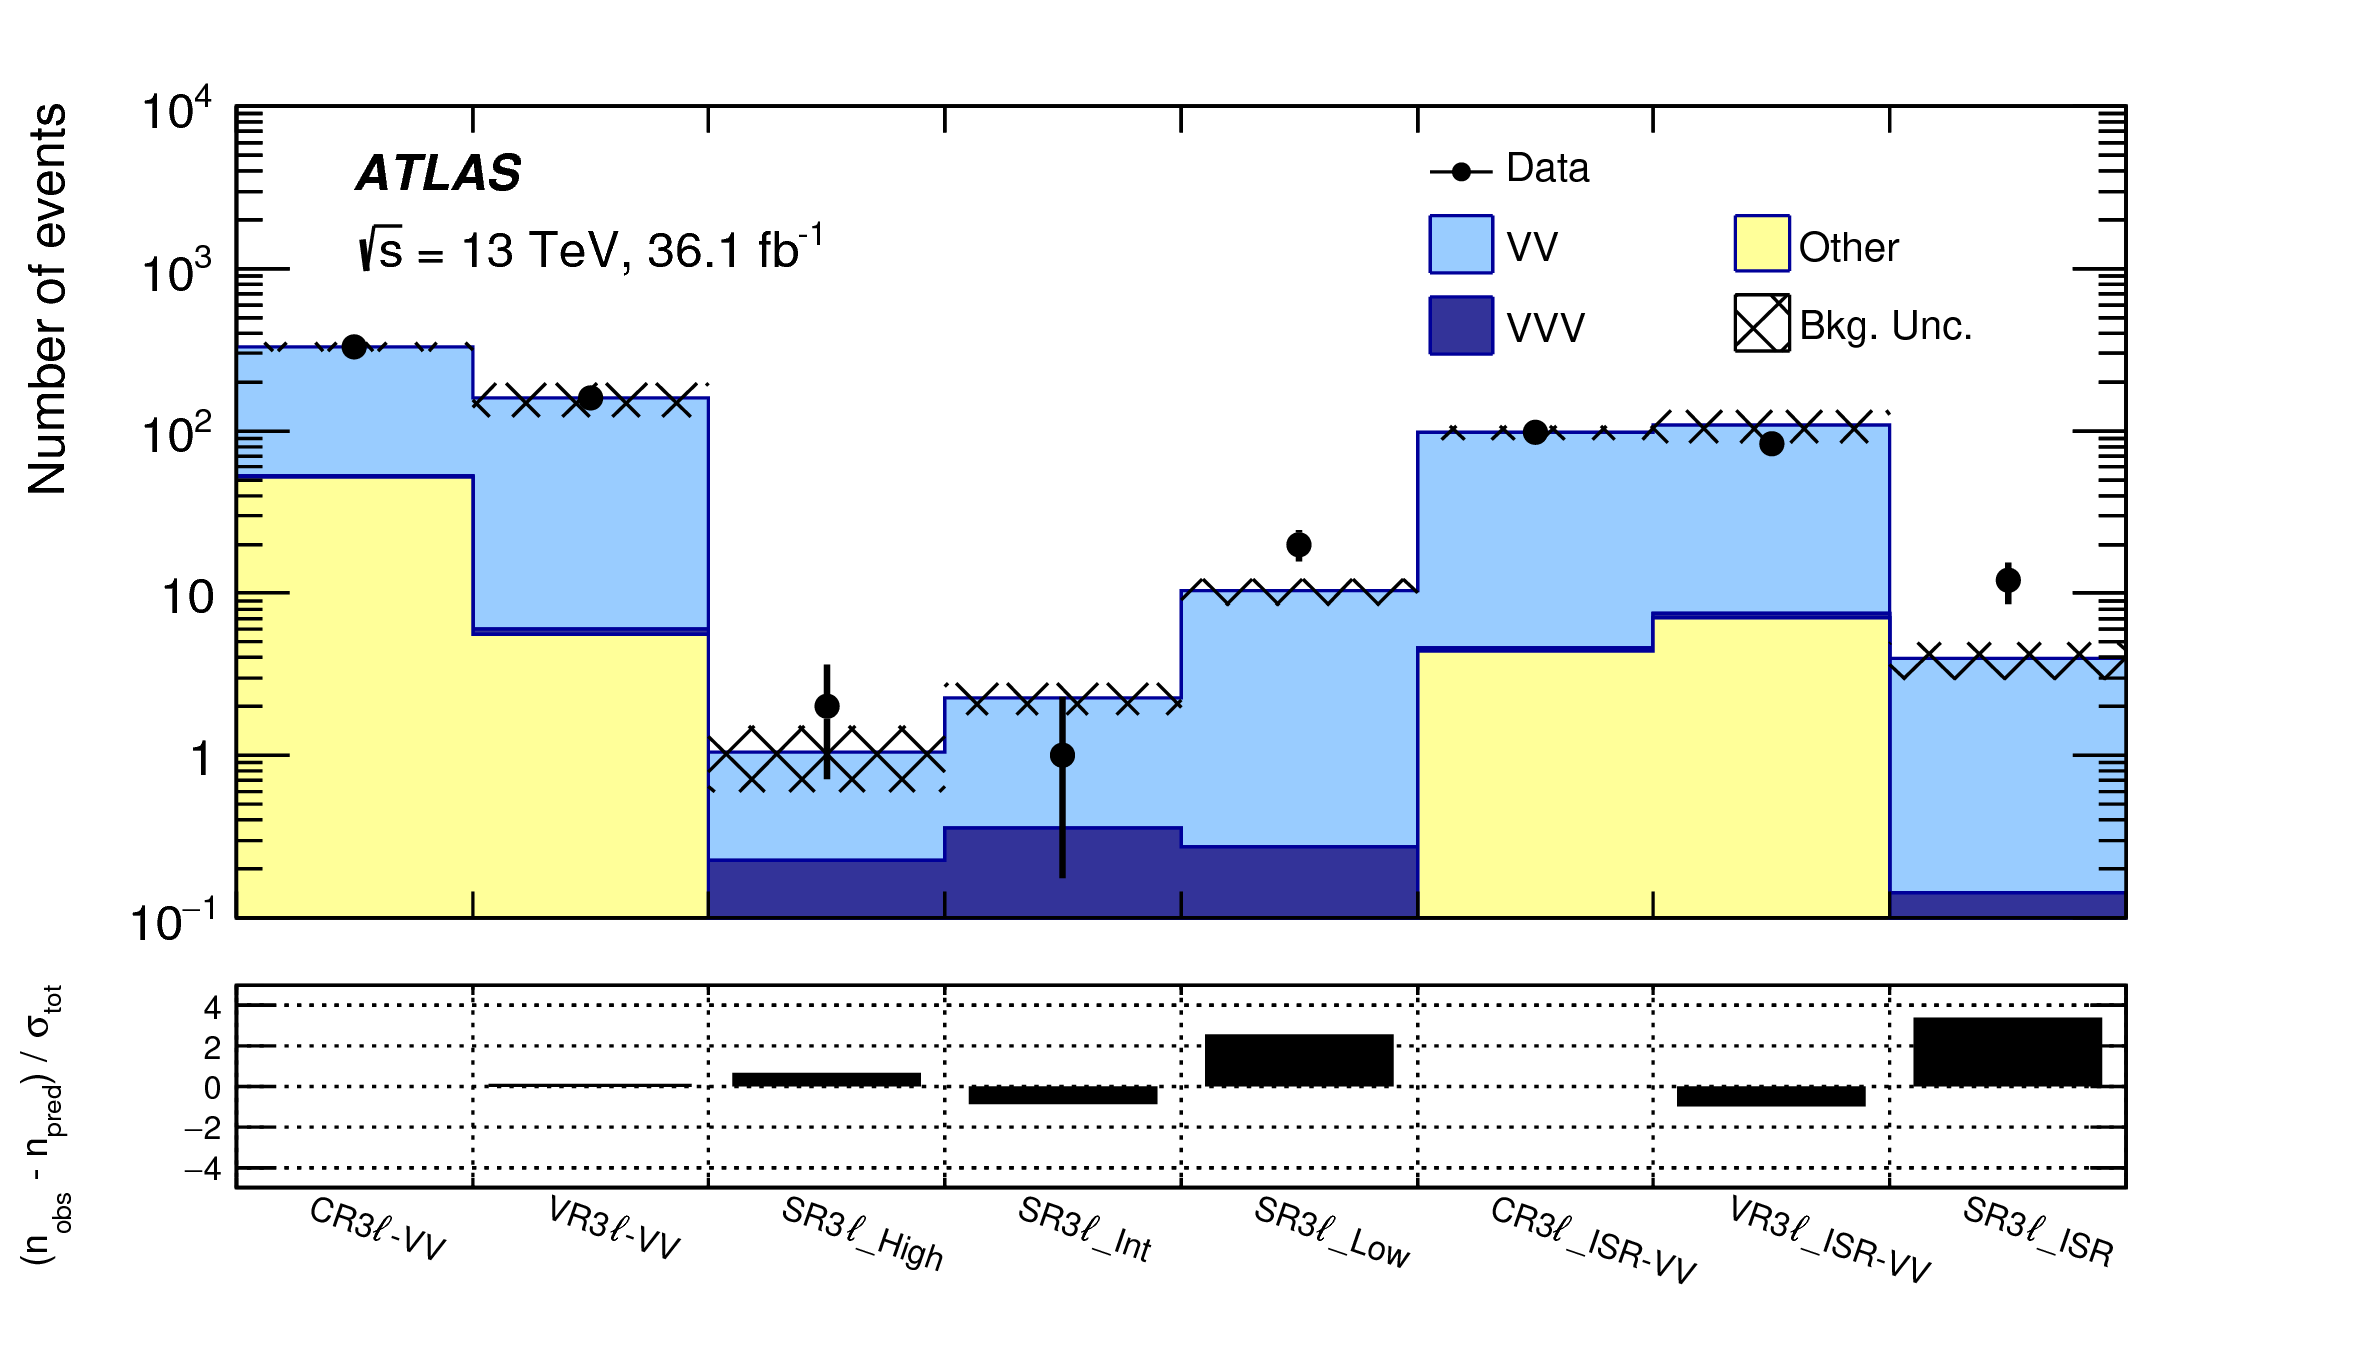
\includegraphics[width=\textwidth]{figures/2ljets_rjr_23l_3l_summary.png}
\caption{$3\ell$ RJR~\cite{atlas_rjr_23l_SUSY_2017_03}}
\end{subfigure}
\\[0.5em]
\begin{subfigure}{0.8\textwidth}
\centering
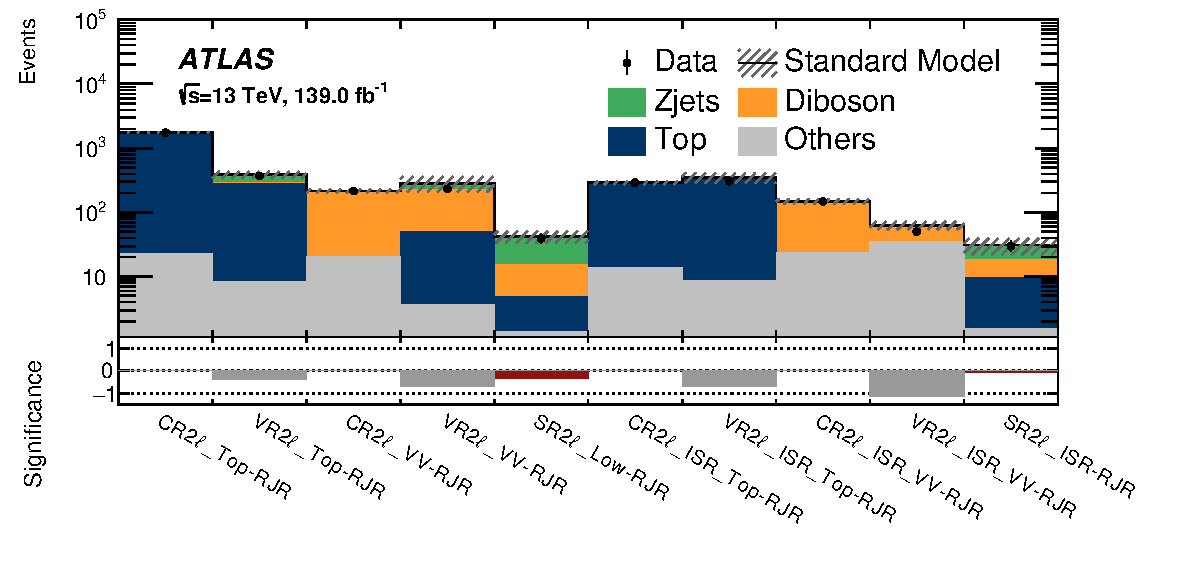
\includegraphics[width=\textwidth]{figures/2ljets_rjr_summary_log.pdf}
\caption{$\twoljets$-RJR~\cite{atlas2022searches}}
\end{subfigure}
\caption[
Summary plots for RJR analyses
]{%
Summary plots for RJR analyses:
(a) and (b)~two- and three- lepton selections respectively,
\emph{reproduced from}~\cite{atlas_rjr_23l_SUSY_2017_03},
(c)~all regions from the $\twoljets$-RJR search~\cite{atlas2022searches}.
Note the excesses in
$\mathrm{SR}2\ell\_\mathrm{Low}$ and $\mathrm{SR}2\ell\_\mathrm{ISR}$ of (a),
and in
$\mathrm{SR}3\ell\_\mathrm{Low}$ and $\mathrm{SR}3\ell\_\mathrm{ISR}$ of (b).
\emph{Sub-figure (c) was made by the RJR team.}
}
\label{fig:2ljets_rjr_summaries}
\end{figure}


\subsubsection{Doubts}
Disappearing excesses have encouraged some doubts about RJR variables in
certain social circles;
the existence of the `RJR-mimic' paper~\cite{atlas_rjr_mimic_SUSY_2018_06}
is public evidence of this.

A more precisely framed problem with RJR variables is that they tend to select
phase space, which is poorly modelled by simulations.
This is plausibly explained by the fact that RJR variables are non-trivially
related to conventional, lab-frame variables.
Simulations have been tuned to model conventional variables well, and
`systematic' variations are evaluated and derived in conventional variables.
Modelling these features accurately does not imply that all other functions of
the data are well understood.
These effects cause Monte Carlo simulations to give predictions in RJR regions
which are inaccurate and/or carry large uncertainties.

A lack of reliable simulations motivates reliance on `data-driven' background
estimates in RJR selections, which, from my perspective, are hard to interpret
or trust.
Indeed, I argue that all `data-driven' methods rely not only on data but on
hypothetical extrapolations which may not be well motivated, particularly when
studying complicated features such as RJR variables.
For these reasons, I choose to not use any RJR event variables in the
$\twoljets$-electroweak analysis.


\FloatBarrier
\subsection{Strong}
\label{sec:2ljets_origins_strong}
Strong supersymmetry, producing super-partners of quarks and gluons, would be
produced at much larger cross-sections than electroweak supersymmetry at the
LHC.
Squarks and gluinos are therefore excluded with masses up to several
$\eV[T]$ using hadronic data alone, depending on which simplified model is
considered~\cite{atlas_susy_strong_0l}.

The $\twoljets$-strong search targets strongly interacting supersymmetric
effects in cases where their decays produce pairs of charged leptons.
Like the RJR and electroweak $\twoljets$ searches, the $\twoljets$-strong
signals produce jets and invisible lightest supersymmetric particles.
Unlike the RJR and electroweak parts, not all of these leptons are produced
by $Z$ boson decays.
As illustrated in Figure~\ref{fig:2ljets_strong_signal_diagrams}, decay trees
featuring sleptons can also produce lepton pairs.
Lepton pairs produced in these slepton interactions are of the same flavour
and opposite charge, like those from $Z$ boson decays, but they have different
mass dilepton mass characteristics.

% signal models
\begin{figure}[tp]
\centering
\begin{subfigure}{0.48\textwidth}
\centering
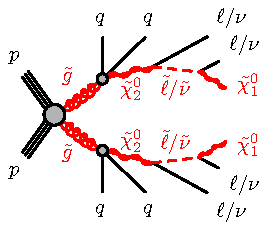
\includegraphics[width=\textwidth]{figures/2ljets_strong_gogo_qqqqllllN1N1_N2.pdf}
\caption{gluino-slepton}
\end{subfigure}
\hfill
\begin{subfigure}{0.47\textwidth}
\centering
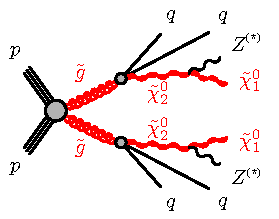
\includegraphics[width=\textwidth]{figures/2ljets_strong_gogo_qqqqZZN1N1.pdf}
\caption{gluino-$Z^{(*)}$}
\end{subfigure}
\\[0.5em]
\begin{subfigure}{0.48\textwidth}
\centering
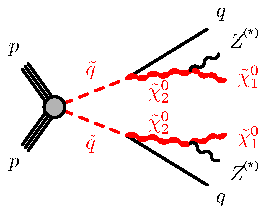
\includegraphics[width=\textwidth]{figures/2ljets_strong_sqsq_qqZZN1N1.pdf}
\caption{squark-$Z^{(*)}$}
\end{subfigure}
\caption[
Supersymmetric signal processes in the $\twoljets$-strong search
]{%
Supersymmetric signal processes in the $\twoljets$-strong search.
\emph{Figures reproduced from the paper%
}~\cite{atlas2022searches, atlas_susy_feynman}.
\\[0.5em]
All models produce same-flavour, opposite-sign lepton pairs along with jets
and $\met$.
The gluino-slepton model (a) has a kinematic endpoint in $\mll$
given in Equation~\ref{eqn:2ljets_strong_max_mll}.
The gluino-$Z^{(*)}$ and squark-$Z^{(*)}$ models decay via $Z$ boson
resonances, which may be forced off-shell for small mass-splittings
$m(\neutralino_2) - m(\neutralino_1) < m(Z)$.
}
\label{fig:2ljets_strong_signal_diagrams}
\end{figure}

Rather than peaking at a resonance mass, these pairs have an $\mll$
distribution with a signature end-point which depends on the masses of other
supersymmetric particles in the
$\neutralino_2 \ldots \slepton \ldots \neutralino_1$
decay chain~\cite{paige1996determining}:
\begin{equation}
\label{eqn:2ljets_strong_max_mll}
\max \mll
= m(\neutralino_2)
\sqrt{1 - \frac{m(\slepton\,)^2}{m(\neutralino_2)^2}}
\sqrt{1 - \frac{m(\neutralino_1)^2}{m(\slepton\,)^2}}
.
\end{equation}

Various previous incarnations of this search have been conducted with similar
selections and target models on in older data, including partial Run~2~\cite{
atlas_susy_strong_2l_partial_run2_1,
atlas_susy_strong_2l_partial_run2,
cms_susy_2016_strong_2l_run2_1,
cms_susy_2016_strong_2l_run2
} and Run~1~\cite{
atlas_susy_strong_2l_run1,
cms_susy_2016_strong_2l_run1
} in \atlas\ and \cms.
From these Run~1 searches, one can cherry-pick excesses
of ``$3.0$ standard deviations'' in \atlas~\cite{atlas_susy_strong_2l_run1}
and ``$2.6$ standard deviations'' in \cms~\cite{cms_susy_2016_strong_2l_run1}.
These excesses of data above estimated backgrounds were not reproduced in their
early Run~2 updates.

% exclusion plots
\begin{figure}[tp]
\centering
\begin{subfigure}{0.48\textwidth}
\centering
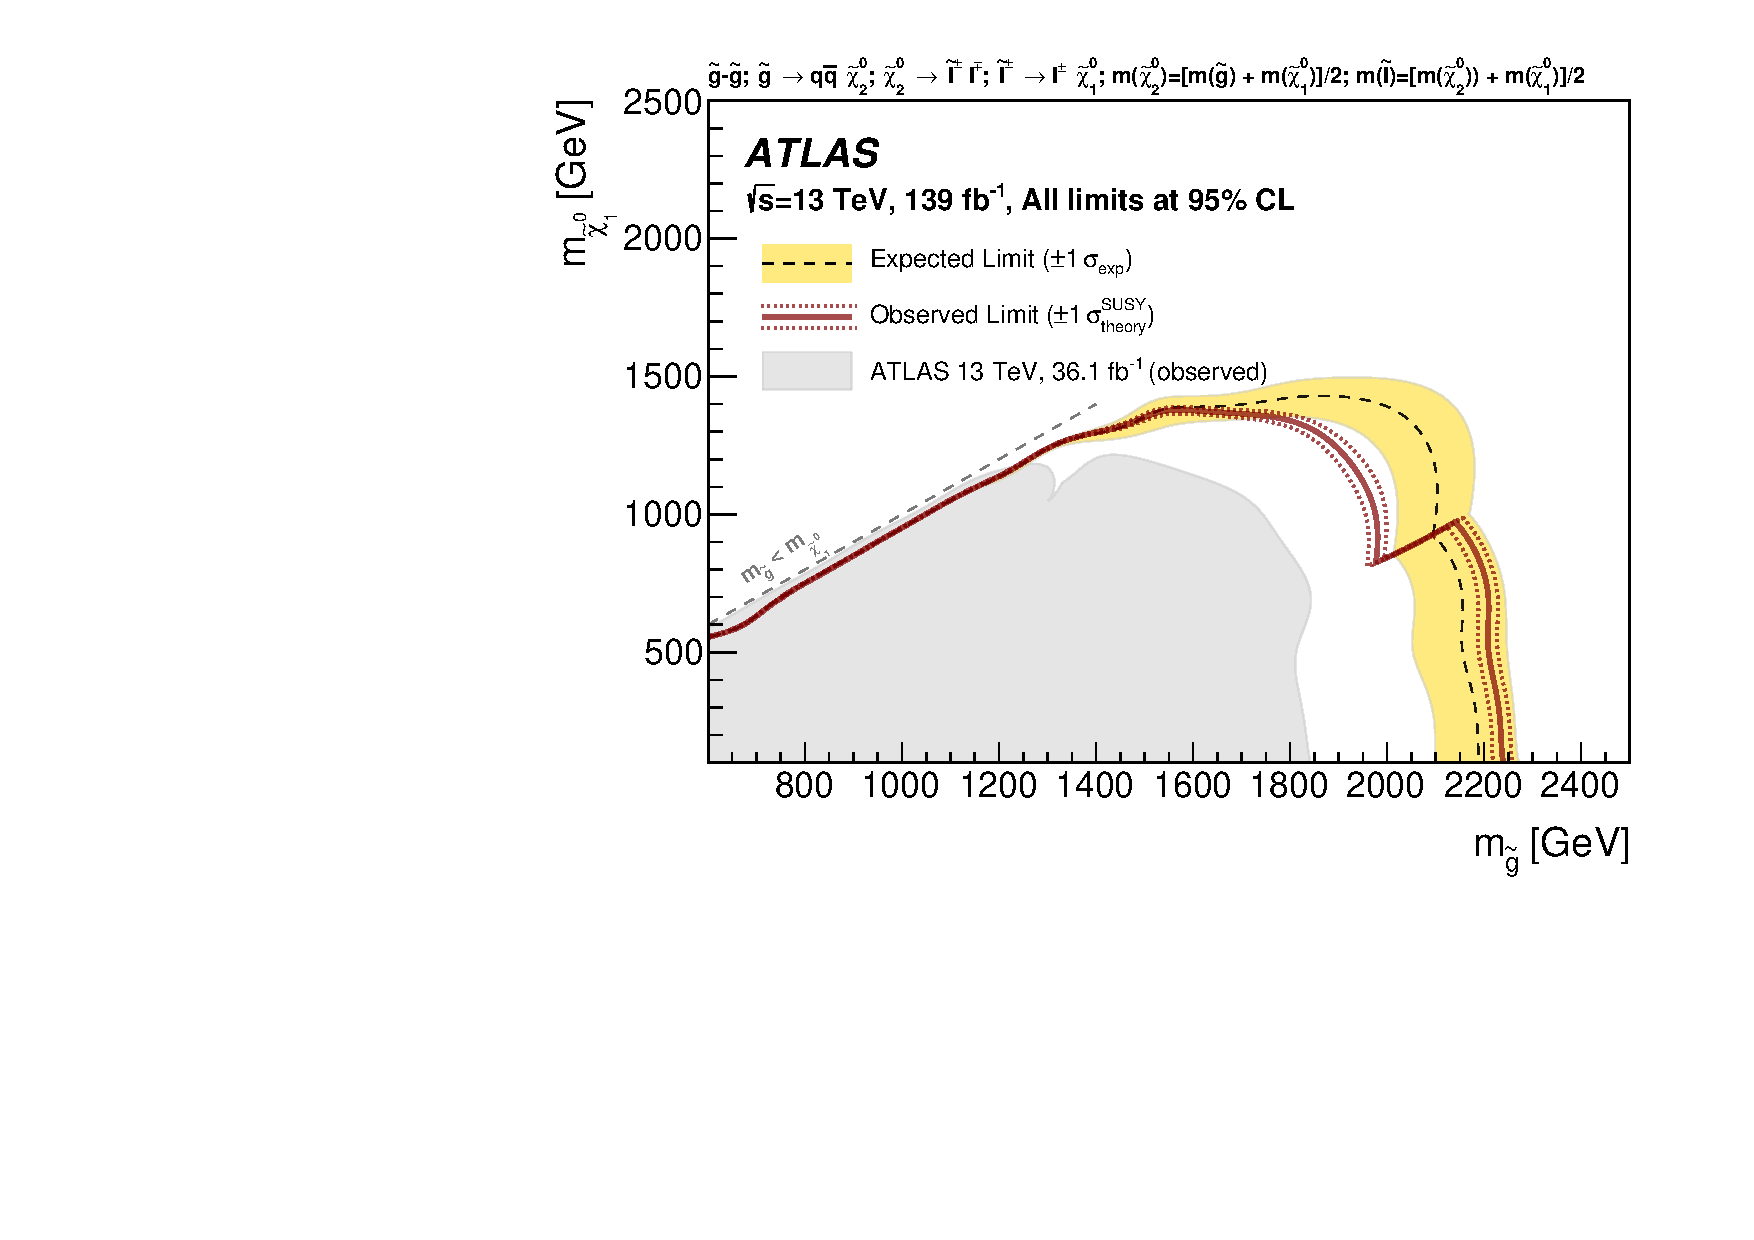
\includegraphics[width=\textwidth]{figures/2ljets_strong_contours_gluino_slepton.pdf}
\caption{gluino-slepton}
\end{subfigure}
\hfill
\begin{subfigure}{0.48\textwidth}
\centering
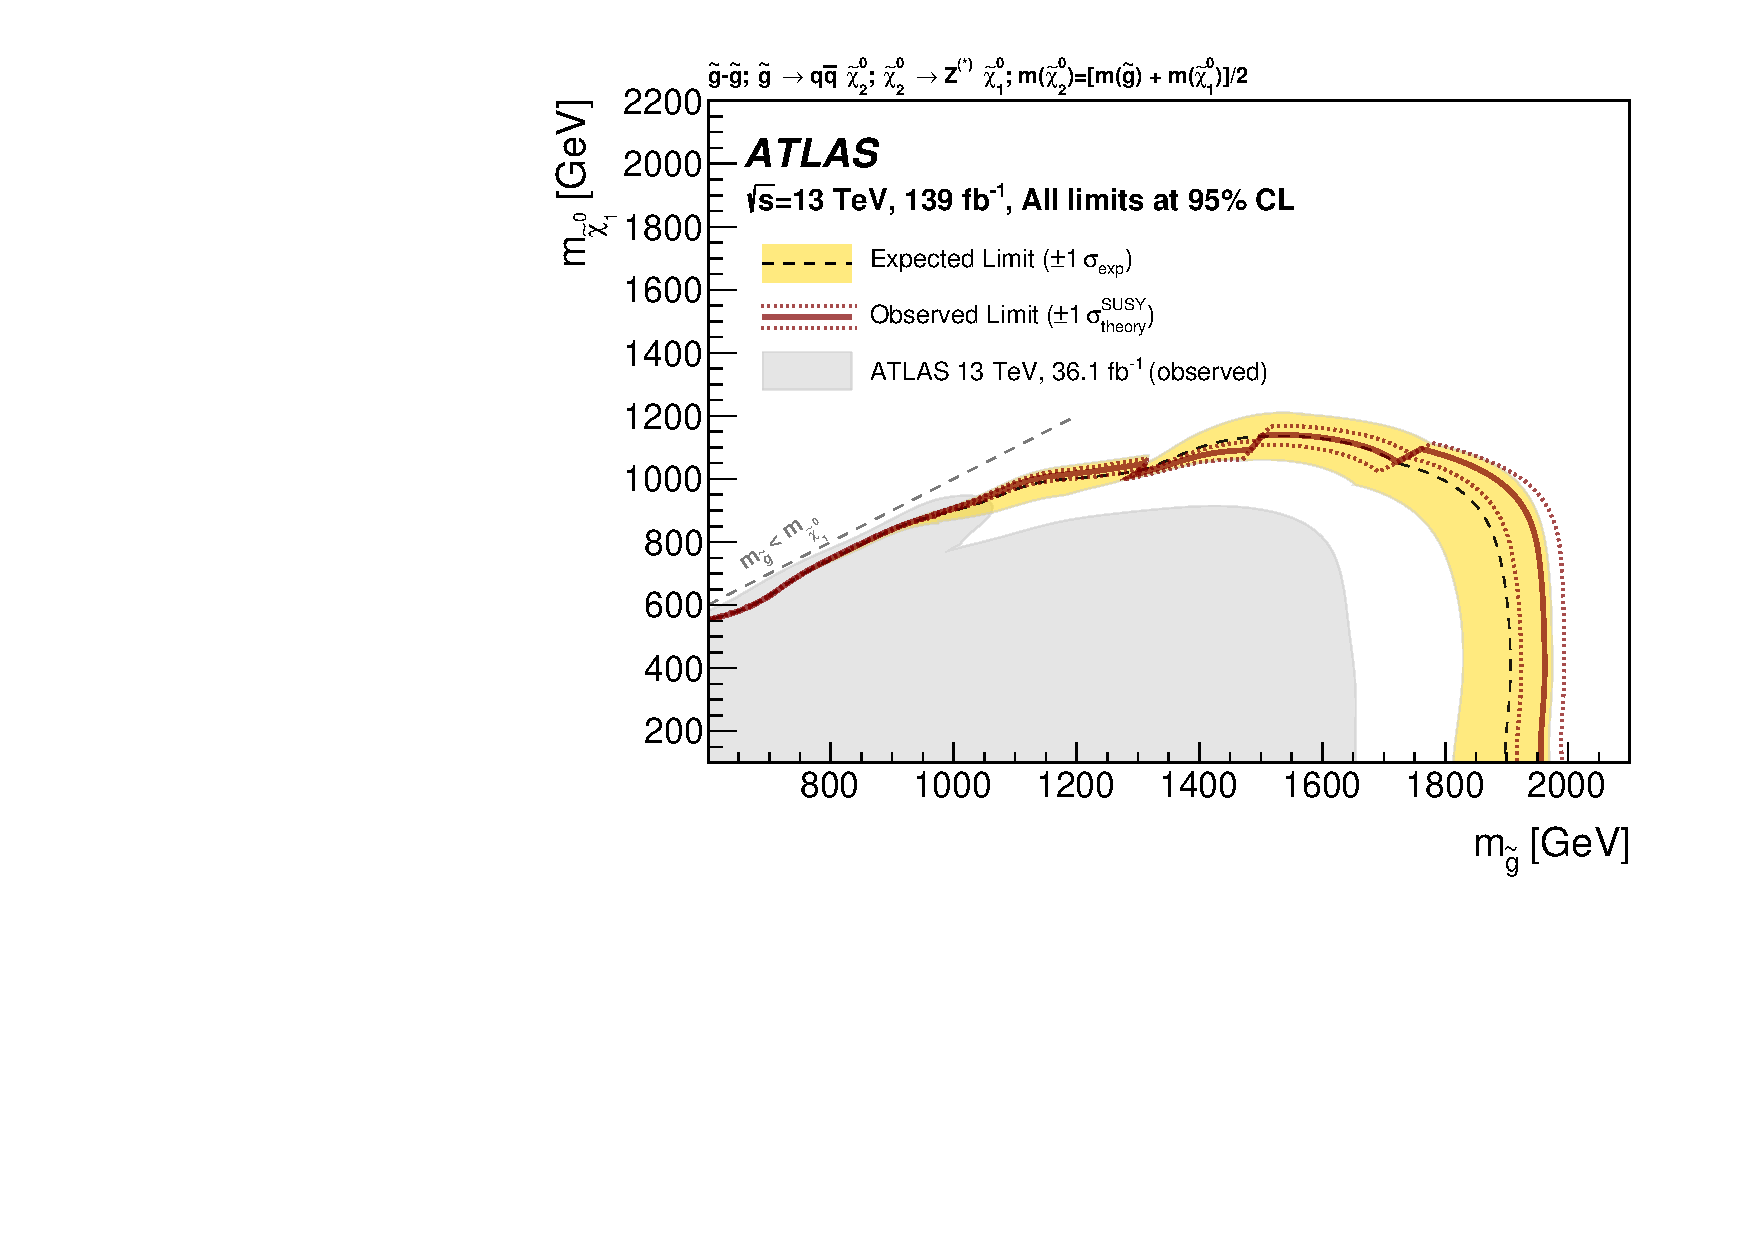
\includegraphics[width=\textwidth]{figures/2ljets_strong_contours_gluino_z.pdf}
\caption{gluino-$Z^{(*)}$}
\end{subfigure}
\\[0.5em]
\begin{subfigure}{0.48\textwidth}
\centering
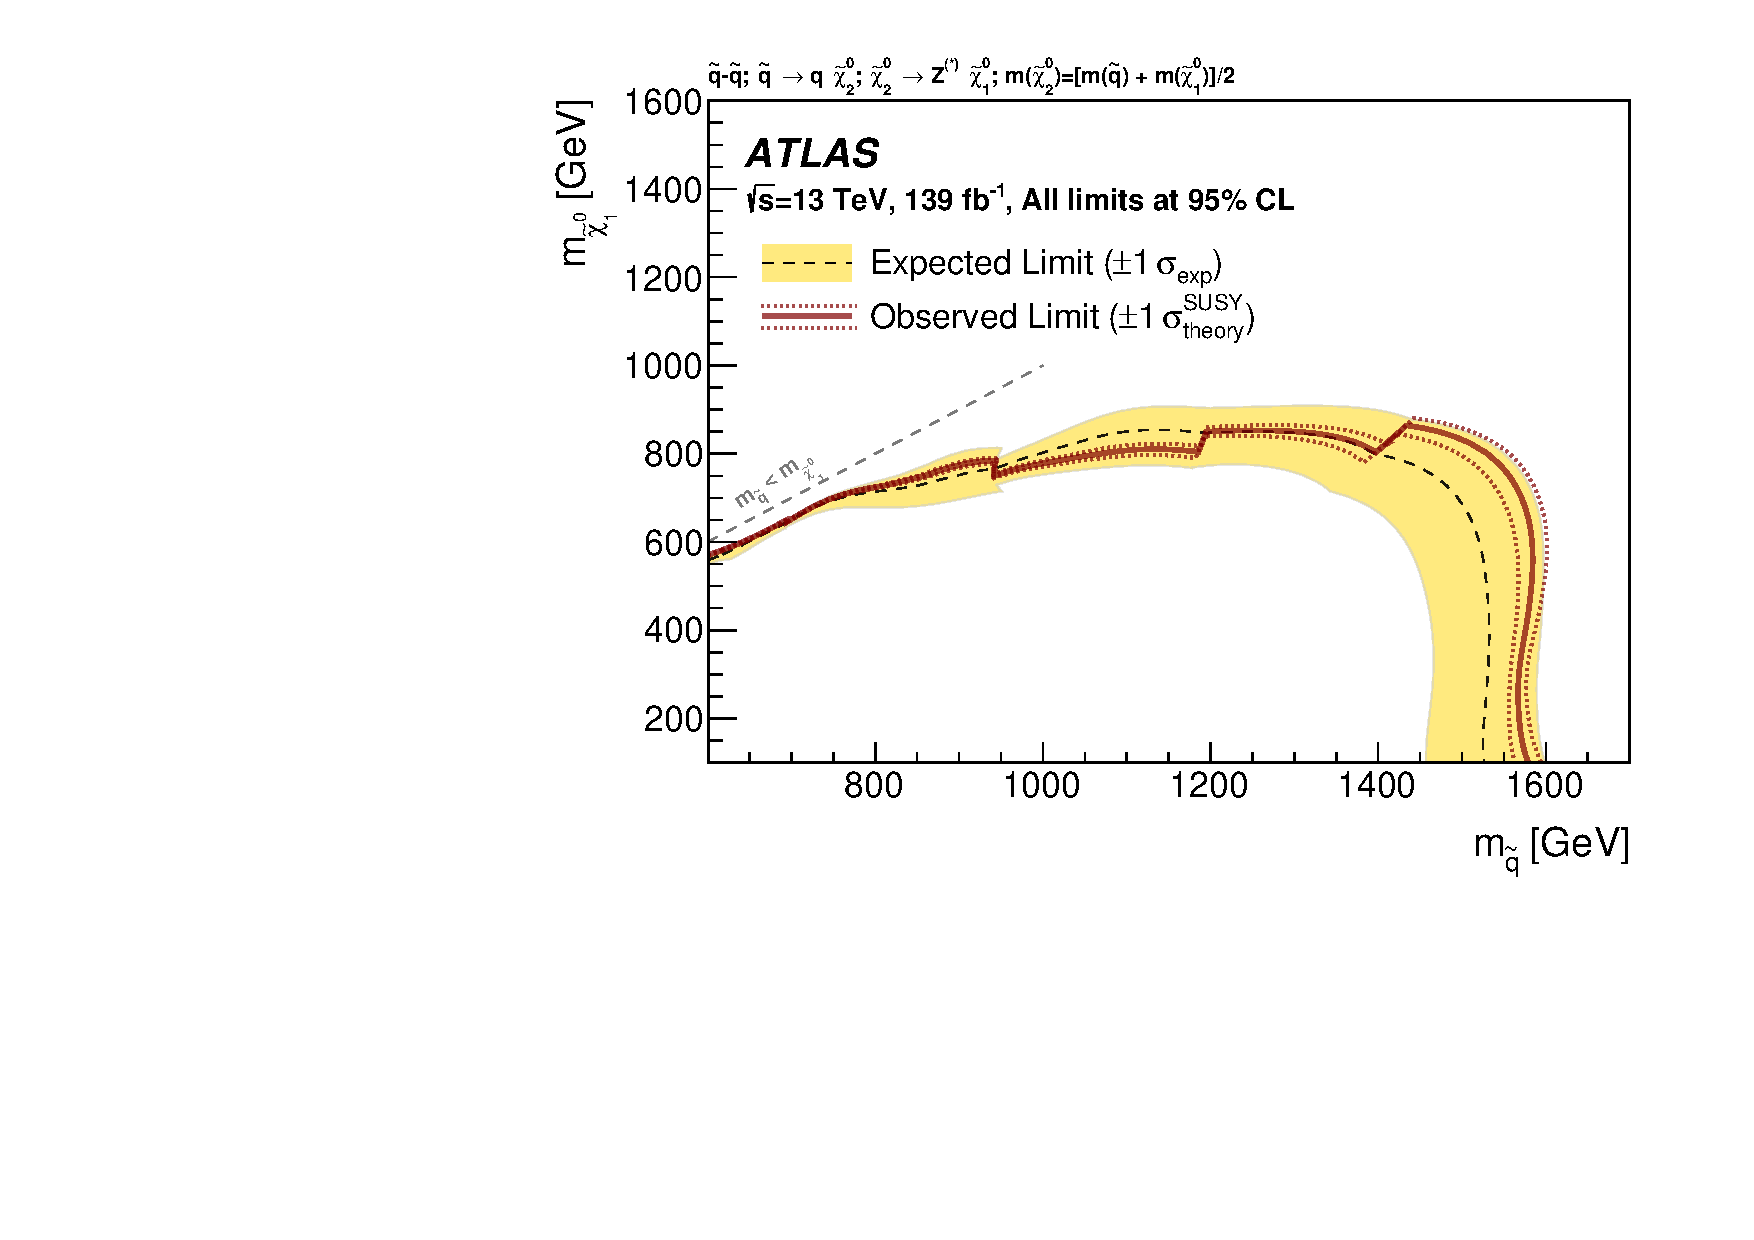
\includegraphics[width=\textwidth]{figures/2ljets_strong_contours_squark_z.pdf}
\caption{squark-$Z^{(*)}$}
\end{subfigure}
\caption[
Contours for signal models of the $\twoljets$-strong search
]{%
Contours for signal models of the $\twoljets$-strong search.
\emph{Figures were produced by the strong team%
}~\cite{atlas2022searches}.
\\[0.5em]
Each model point uses fit results from the signal region with the
``best expected sensitivity'';
jagged edges arise from the switching between contours set by these different
signal regions.
The grey shaded contours showing previous exclusion are taken
from~\cite{atlas_susy_strong_2l_partial_run2}.
}
\label{fig:2ljets_strong_contours}
\end{figure}

To target its signal models, $\twoljets$-strong search defines seven
overlapping signal regions.
Three target on-shell $Z^{(*)}$ models by selecting $\mll$ close to $m(Z)$,
and the others are binned in $\mll$ to give broad sensitivity to the various
kinematic edges across the grid of signal model parameters.

The largest Standard Model background to this search is dileptonic $\ttbar$,
in part because no $b$-jet veto is used.
All three signal models produce same-flavour lepton pairs, but $\ttbar$
produces same-flavour ($ee$/$\mu\mu$) and different-flavour ($e\mu$) pairs at
equal rates.
This difference in flavour symmetry is exploited to estimate backgrounds in
$\twoljets$-strong,
and its previous iterations~\cite{cms_susy_2016_strong_2l_run2_1}.
The estimate works by taking different-flavour data, weighting them by factors
to calibrate for differences in the leptons' reconstruction, and histogramming
them in same-flavour regions.
Simulations for $\ttbar$ and the smaller flavour symmetric backgrounds
$tW$, $WW$, and $\tau\tau$ are replaced by this estimate.

Post-fit results match the data to within $1$-sigma in all $\twoljets$-strong
regions.

Exclusion contours from the $\twoljets$-strong search are reproduced in
Figure~\ref{fig:2ljets_strong_contours}.
Besides their increased reach, the jagged edges to parts of these contour are
striking.
These arise from the combination of results from overlapping signal regions.
Because they overlap, they are not independent and cannot be trivially
combined.
Instead, each model in the signal grid is assigned to the signal region
with the ``best expected sensitivity'' by some measure.
An exclusion contour is constructed for each signal region, then those contours
are joined such that models assigned to each region use its corresponding
contour.

Personally, I find this hard to interpret.
If I had a pet theory which landed near to one of these sharp
region-transition edges, what should I make of these data?
Could some combination of the regions not have combined their information to
produce more precise contours?
Since model predictions change continuously, should our inferences not also?
To aid interpretations and to allow combinations of regions'
information, I chose to design the $\twoljets$-electroweak with only orthogonal
regions, and without any manual switching of regions between models.


\FloatBarrier
\subsection{Electroweak}
\label{sec:2ljets_origins_electroweak}
As motivated in the previous sections, I have personal preferences for
simulation-driven backgrounds and orthogonal multi-bin regions.
This is because simulation-driven estimates are interpretable as
Standard Model predictions,
and orthogonal regions have independent likelihoods which can be cleanly
combined to leverage the information in their data.

The main idea behind the design of the $\twoljets$-electroweak analysis is to
update the regions of the partial Run~2 search in its $\twoljets$
channel~\cite{atlas_23l_SUSY_2016_24}, which also searched for signal models
producing chargino-neutralino pairs which decay via $W$ and $Z$ bosons.
A particular goal was to improve sensitivity by replacing their overlapping
`SR2-int' and `SR2-high' regions with orthogonal selections.
\emph{I am grateful to Sarah Williams for suggesting this approach.}

As in the $\twoljets$-strong search, the partial Run~2 search chose one
signal region from an expected sensitivity for each signal point,
as displayed in
Figure~\ref{fig:2ljets_23l_stuff}
with the two regions and exclusion contours.

\begin{figure}[tp]
\centering
\begin{subfigure}{0.6\textwidth}
\centering
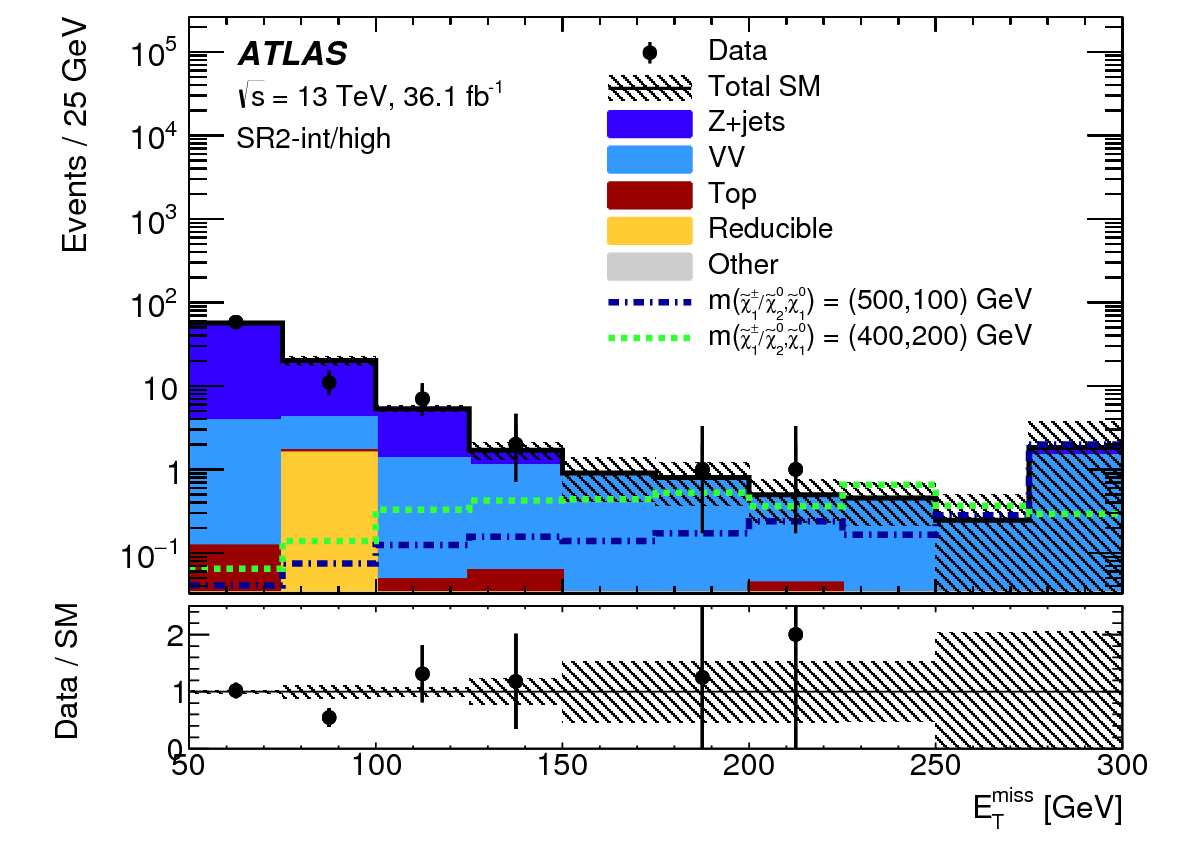
\includegraphics[width=\textwidth]{figures/2ljets_23l_sr2inthigh.png}
\caption{SR2-int and SR2-high}
\end{subfigure}
\\[0.5em]
\begin{subfigure}{0.52\textwidth}
\centering
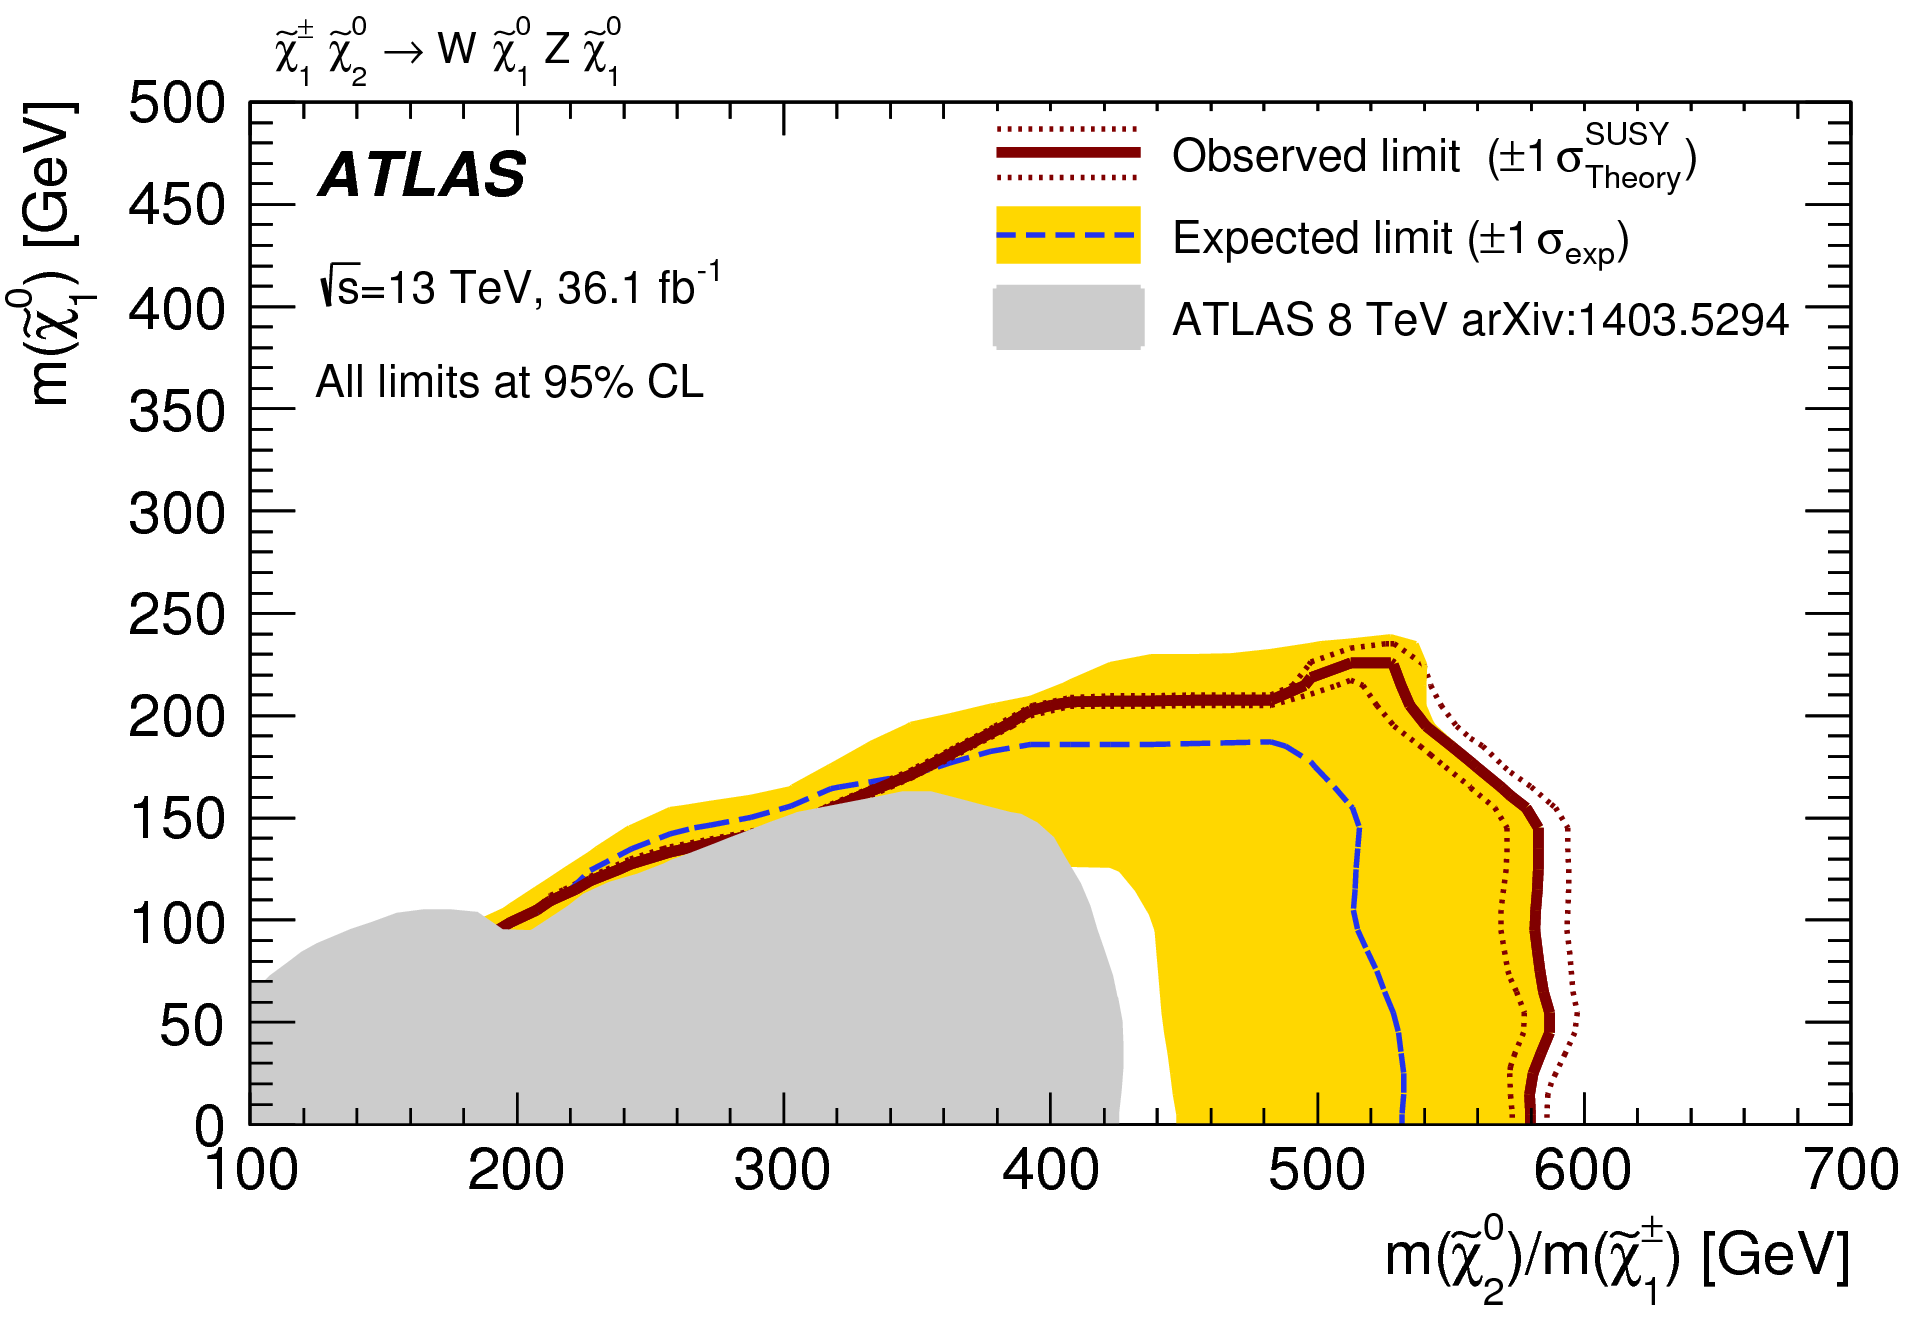
\includegraphics[width=\textwidth]{figures/2ljets_23l_contours_fig_08d.png}
\caption{Combined exclusion}
\end{subfigure}
% \hfill
\begin{subfigure}{0.46\textwidth}
\centering
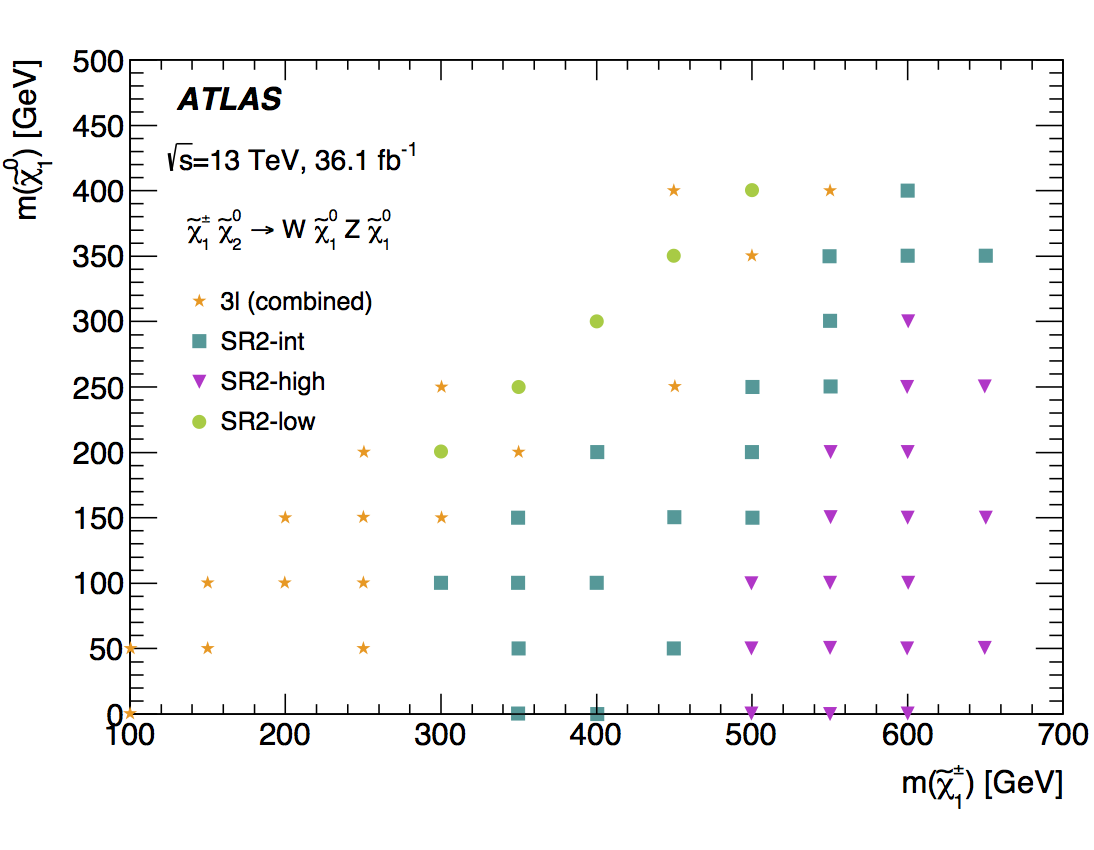
\includegraphics[width=\textwidth]{figures/2ljets_23l_chosen_regions.png}
\caption{Chosen regions}
\end{subfigure}
\caption[
Figures reproduced from the partial Run~2 search with $2/3\ell$ selections
]{%
Figures reproduced from the partial Run~2 search with $2/3\ell$
selections~\cite{atlas_23l_SUSY_2016_24, hepdata.81996}.
\\[0.5em]
(a) Histogrammed distribution of $\met$ in and below SR2-int and SR2-high with
example signal models.
SR2-int requires $\met > 150\,\eV[G]$ and SR2-high requires $\met > 250\,\eV[G]$.
\\[0.5em]
(b) Contours for the combined $\twoljets$ and $3\ell$ channels.
Each signal point chooses a signal region, which is displayed in (c).
The grey region shows exclusion from a previous search in Run~1
data~\cite{atlas_2l_SUSY_2013_11}.
\\[0.5em]
(c) Signal regions selected for each signal point in the grid.
Two-lepton selections occupy the largest mass-splittings.
The $3\ell$ regions are orthogonal and combined.
}
\label{fig:2ljets_23l_stuff}
\end{figure}

Additionally, $\twoljets$ widens its scope to target a GMSB simplified model
illustrated in Figure~\ref{fig:2ljets_signal_diagrams}.
The C1N2 and GMSB models behave similarly since both feature decays via massive
bosons ($WZ$, $ZZ$ or $Zh$) to leptons and jets, in similarly structures decay
trees to pairs of invisible supersymmetric particles.
Although widening sensitivity to both models does sacrifice sensitivity to
either one, the increased degree of model independence is itself of value for
future reinterpretations of the data.
We are happy to sacrifice some precision for generality.

Multi-bin fits are not special.
They are standard \atlas\ practice, and there could have been no complication
in replacing the overlapping SR2-int and SR2-high with orthogonally binned
regions.
However, my design decisions for $\twoljets$-electroweak
caused problems for the clarity of communication and accuracy of background
modelling.
These issues are developed further through the remainder of this chapter.

A multi-binned histogram is usually and clearly illustrated as slicing up one
variable.
My design of $\twoljets$-electroweak violates this.
Instead, it is designed as a tree whose branches recursively split various
variables.
This leads to specifications which are challenging to present and understand,
and which require region names with numerous suffixes to specify where they
live in that tree.

Worse, I disregarded the idea that every region should have a large
background expectation.
Normally, this is justified by the limitations of approximate statistical
methods, which work
``from as few as $\mathcal{O}(10)$ data events''~\cite{histfitter2014}.
But the Poisson likelihood works for infinitesimally small
expectations~\cite{skilling2009cosmology}, and in the small-bin limit one has
continuous distributions
(sometimes called ``extended''~\cite{barlow1990extended}),
which are standard and easily analysed.

Events appearing in a region with minimal background is evidence in favour
of new contributions, and that only strengthens as the background approaches
zero.
For example, the top quark was observed by \dzero\ using seven regions all with
background expectations of $1$ or less, for a total of $3.79\pm0.55$ expected
and $17$ observed~\cite{abachi1995observation}.
If they could do that with technology from the year $1995$, we can do it now.

The real reason to avoid small backgrounds is, in this context, to allow honest
assignments of background uncertainties.
Although main simulated samples may have good precision,
many `systematic' variations and `data-driven' estimates are also required.
Many of these alternative estimates have far worse precision, and can fail
totally as the number of simulated events accepted plunges towards zero;
they can require $\approx10$ data events to work properly.

Unfortunately, $\twoljets$-electroweak selections were finalized before I
appreciated this problem that background variations were dubious.
Various workaround are invoked to assign plausible variations despite small
yields, which we shall in the remainder of this chapter.

As seen in the splash summary of Section~\ref{sec:2ljets_splash}, this search
finds agreement with backgrounds except for some local deficits of data below
backgrounds.
Exclusion contours exceed their expected range because of these deficits,
but they can only be trusted if the background model is trusted.

Searches have been performed in \cms\ for similar
C1N2~\cite{cms_susy_2022_c1n2} and GMSB models~\cite{
cms_susy_2018_partial_run2_combination,
cms_susy_2022_gmsb
}, with comparable results.

\TODO{other atlas C1N2 and GMSB searches (combinations, 3L offshell exclusion)}


\section{Events}
This section describes the events selected for the $\twoljets$ searches, the
reconstructed particle objects derived from those events and various
important event variables.

From its name, it is clear that $\twoljets$ analyses features of events with
two charged leptons (electrons or muons --- not taus), and at least one jet.
Though not nominal, a $\met$ requirement is also implicit from the context
of $R$-parity conserving supersymmetric models.
This section serves to describe how events are selected for the $\twoljets$
analyses, and which event variables are extracted for use in its selections.

Triggers and object definitions are shared between the three $\twoljets$
searches.
Higher level event variables and selections will only be described for the
$\twoljets$-electroweak search.

\subsection{Trigger}
\label{sec:2ljets_trigger}
There would be no event variables if not for the trigger.
When living our daily lives, we are bombarded with sensory data and must pay
attention only those gems few of any use, to avoid exhausting our
processing capacity.
Running \atlas\ is no different.

Each trigger in \atlas' arsenal activates on a selection comprising some
combination of sufficiently hard objects.
The set of targeted objects includes all those used in this analysis and more:
electron, muons, jets, $b$-jets, $\met$, as well as photons and hadronically
decaying tau leptons~\cite{atlas_PERF_2007_01}.

The list of available triggers in \atlas\ is designed to balance data rates
against physical interest.
It includes a variety of general purpose selections, which are used for
$\twoljets$, along with more specialized targets such as vector boson fusion
or long-lived particles.
The list varies through time, so we select triggers specifically in
each data-taking period.

The loosest triggers are `prescaled' --- their data rate is reduced by randomly
accepting only a small fraction of events.
Prescaling adds complication which we avoid;
for $\twoljets$, we use only the `lowest' (loosest, highest rate) un-prescaled
triggers selecting two charged leptons~\cite{atlas_twiki_lowest_unprescaled}.
Those charged leptons are selected in the
high-level trigger (described in Section~\ref{sec:atlas_trigger})
primarily requiring large $\pt$ and certain quality criteria which vary by
trigger.

In total, we use $14$ different two-lepton trigger selections, each of which
selects for an electron pair, a muon pair, or an emu (electron-muon pair).
To describe those triggers, let $\pt^{\ell_i}$ be the transverse momentum of the
$i\mathrm{th}$ hardest lepton.

In short, all triggers require $\pt^{\ell_i}$ values to exceed thresholds in
the range $8\textrm{--}26\,\eV[G]$.
To detail all trigger requirements and their variations with data period
would be too tedious and not enlightening, but their $\pt^{\ell_i}$ requirements
are summarized here.
Please do not read them all in detail.
\begin{itemize}
\item Electron pair: requirements vary between
\begin{itemize}
\item $\pt^{e_2} > 12\,\eV[G]$ and
\item $\pt^{e_2} > 17\,\eV[G]$.
\end{itemize}
\item Muon pair: various requirements include
\begin{itemize}
\item $\pt^{\mu_2} > 10\,\eV[G]$,
\item $\pt^{\mu_2} > 14\,\eV[G]$,
\item $\pt^{\mu_1} > 18\,\eV[G]~\&~\pt^{\mu_2} > 8\,\eV[G]$, and
\item $\pt^{\mu_1} > 22\,\eV[G]~\&~\pt^{\mu_2} > 8\,\eV[G]$.
\end{itemize}
\item Emu pair: various asymmetric requirements include
\begin{itemize}
\item $\pt^{e_1} > 17\,\eV[G]~\&~\pt^{\mu_1} > 14\,\eV[G]$,
\item $\pt^{e_1} > 7\,\eV[G]~\&~\pt^{\mu_1} > 24\,\eV[G]$, and
\item $\pt^{e_1} > 26\,\eV[G]~\&~\pt^{\mu_1} > 8\,\eV[G]$.
\end{itemize}
\end{itemize}
The point of listing these is to demonstrate trigger activations are
non-trivial.
This motivates lepton selections which exceed these trigger thresholds,
to avoid the need to model their jagged activations and variable
efficiencies near to those thresholds~\cite{
atlas_trigger_egamma_run2,
atlas_trigger_muon_run2
}.
Throughout the data used in $\twoljets$, trigger requirements
have increased in hardness with time.


\subsubsection{Alternative triggers}
Why should we only use two-lepton triggers?
Alternatives could be one-lepton triggers, for cases where the other is not
reconstructed at trigger level, or perhaps also triggers for jets and $\met$.
The answer is that the benefits of additional triggers were assessed to not
outweigh the cost of using them.

The benefit of an additional trigger could be in increased signal yields if
that trigger does not also harmfully increase inseparable backgrounds.
A study, \emph{which was performed by Knut Vadla}, investigated the effects
of including one-lepton triggers.
In a signal-region-like selection requiring two leptons, two jets and
$\met > 200\,\eV[G]$, this study showed that two-lepton triggers already accept
in excess of $90\%$ of events from benchmark C1N2 models.
Therefore, any additional trigger has at most a $\approx10\%$;
improvement. Adding one-lepton triggers was found to increase efficiency by
only a few percentage points, depending on the model.
We considered that to be too little to be worthwhile.

Costs of triggers are attributable to human effort;
software work to include them and their associated Monte Carlo weights, along
with studies to validate background estimates and evaluate systematic
uncertainties.
Similarly, our implementation of the Matrix Method fake/non-prompt lepton
background estimate (see Section~\ref{sec:2ljets_mm_fakes}) is not equipped to
handle one-lepton triggers.

Although jet and $\met$ triggers were not studied in detail, they can be
quickly ruled out since they hard objects: examples of these triggers require
approximately $\ptjone > 400\,\eV[G]$, $p_\mathrm{T}^{\,j_3} > 200\,\eV[G]$, or
$\met > 100\,\eV[G]$~\cite{atlas_twiki_lowest_unprescaled}.
Leptons, however, are striking signals which are produced as smaller background
rates, as they suppressed by electroweak couplings.
Therefore, \atlas\ can trigger on leptons with much softer requirements;
lepton triggers allow us to use softer jets and $\met$, which are relied upon
throughout the $\twoljets$ analyses.


\subsection{Leptons}
In the context of $\twoljets$, `leptons' means `electron-or-muons';
this is because taus, which decay before reconstruction, and are not used
directly in $\twoljets$, and neutral leptons (the neutrinos) go missing.

Reconstructed lepton objects feature momenta, charges, and flavours.
Each is included only if it satisfies certain kinematic and
is identified with `quality' criteria.
For both electron and muons, these criteria are standardized with labels
`loose', `medium', and `tight'.
These are nested, in the sense that tight implies medium,
and medium implies loose.
Other, more specialized, criteria exist, but they are not relevant $\twoljets$.

Muons are identified by fitting tracks to hits in the inner tracker and muon
spectrometer.
Their quality criteria use goodness-of-fit metrics from those fits, along with
low-level details of detector interactions.
Tighter requirements primarily act to reduce from non-prompt backgrounds,
which are muons from hadronic decays~\cite{atlas_muon_quality_MUON_2018_03}.

Electron identification combines data from the inner tracker and
calorimeters.
Electron quality criteria use numerous features of detector
interactions, track fitting metrics, the matching of tracks to calorimeter
clusters, calorimeter shower shapes, and leakage into the hadronic calorimeter.
Tighter requirements reduce backgrounds, which include misidentified objects
--- photons and hadrons --- as well as non-prompt electrons from hadronic
decays~\cite{atlas_egamma_quality_EGAM_2018_01}.

Isolation of leptons from nearby hadronic activity is another feature which
can be used to reduce misidentification rates.
Standard isolation definitions exist for both electrons and muons in a similar
structure to the quality criteria.

Leptons in $\twoljets$ are further sliced into two classes:
`baseline' and `signal'.
Baseline leptons and are used in background estimation methods and to ensure
orthogonality with other \atlas\ analyses, which study events with differing
lepton counts.
Baseline requirements are softer and lower quality than signal requirements.

Any event used in regions of the $\twoljets$-electroweak analysis is required
to have exactly two baseline leptons and exactly two signal leptons, meaning
that the event has two reconstructed leptons which pass both sets of criteria.
This vetoes events with soft or low quality third leptons, ensuring that those
three-lepton events can be used independently in other studies.

Baseline leptons are required only to have $\pt > 3\,\eV[G]$ for muons and
$\pt > 4.5\,\eV[G]$ for electrons.
Signal leptons are all required to have $\pt > 10\,\eV[G]$, along with tighter
quality and isolation requirements, details of which are given in the
paper~\cite{atlas2022searches}.
Electrons are accepted within $|\eta| < 2.47$.
Baseline muons have $|\eta| < 2.7$, and signal muons have $|\eta| < 2.6$.


All leptons used in regions of the $\twoljets$-electroweak analysis are signal
leptons with $\pt > 25\,\eV[G]$.
This harder requirement reduces backgrounds, moves our selections away from the
lowest trigger thresholds, and matches the precedent set by previous
work~\cite{atlas_23l_SUSY_2016_24}.


\subsection{Jets}
Like leptons, hadronic jets are identified with `baseline' and `signal'
requirements, with increasingly tight requirements on quality metrics and
kinematics.

Jets in $\twoljets$ use the anti-$k_t$ algorithm with the standard small-radius
parameter of $R=0.4$~\cite{jet_anti_kt}.
Jets are formed from `topological' clusters of energy deposits in the
calorimeters~\cite{atlas_jet_topo_PERF_2014_07}.

This topological clustering algorithm is no longer the \atlas-recommended jet
algorithm; it has been supplanted in recent years by a `particle flow' method,
which uses tracking information to improve the reconstruction of charged
hadrons~\cite{atlas_jet_pflow_PERF_2015_09}.
We did not attempt to switch to these improved jets because the change in
policy occurred during the years this analysis was in development, and the
change would have required more work and even more delays.

Baseline jets are defined to require $\pt > 20\,\eV[G]$ with $|\eta| < 2.8$;
signal jets additionally require $\pt > 30\,\eV[G]$.
To reduce the impact of pile-up jets, a variety of quality criteria are used,
depending on the jet $\pt$ and $|\eta|$.
Details of these quality criteria and angular selections are given in the
paper~\cite{atlas2022searches}.


\subsection{\textit{b}-jets}
\label{sec:2ljets_btagging}
Tagging adds labels to objects.
Unlike how electrons and muons are very cleanly separated, however, jet tagging
is a more noisy affair.
Taggers are available for various jet properties, such charm flavour ($c$-jet),
bottom flavour ($b$-jet).
Of these, $\twoljets$ uses only $b$-tagging.

Larger radius jets can also use taggers for heavy decays, such as those from
$W$, Higgs or top resonance, but large radius were considered too much
additional work to considered in $\twoljets$.

Jets originating from $b$ quarks are distinct due to the long lifetimes and
long decay trees of $B$-hadrons, both of which leave signals in \atlas'
inner trackers.

For jets in $\twoljets$, $b$-tagging is useful to separate events due to
$\ttbar$ backgrounds (since their weak decays almost always produce $b$
quarks), and to select for signals producing $Z/h \rightarrow b\bar b$ decays
in the GMSB model.

Signal $b$-jets in $\twoljets$ require $\pt > 20\,\eV[G]$, $|\eta| < 2.5$ and a
tag from the `MV2c10' boosted decision tree
algorithm~\cite{
friedman2002stochastic,
atlas_jet_mv2c10_2017,
atlas_jet_tagging_2019
} at its $77\%$ efficiency working point.
This efficiency means that a true $b$-jet sampled from its testing set has a
$77\%$ probability of being tagged.
It is trained on a mixture of $\ttbar$ and $\zjets$ simulated data,
and the `c10' suffix means that those data include a $7\%$ fraction of
$c$-jets, and that the tagger does not use newer inputs from the
RNNIP (Recurrent Neural Network Impact Parameter) tagger, nor the
SMT (Soft Muon Tagger)~\cite{atlas_twiki_mv2, atlas_jet_mv2c10_2017}.

This tagging algorithm combines various lower-level features, including the
basic kinematics $\pt$ and $|\eta|$, and more intricate features of
observable secondary vertices including reconstructed hadronic decay
trees~\cite{atlas_jet_mv2c10_2017}.

Alternative working points of $70\%$ and $85\%$ efficiency are used in similar
\atlas\ searches.
These were trialled and found to make negligible differences to $\twoljets$.

An alternative $b$-tagging algorithm named `DL1' is now recommended by \atlas,
but its performance is ``similar'' to MV2, and the two tag
``highly correlated'' samples~\cite{atlas_jet_tagging_2019}, so we did not
attempt to switch.


\subsection{Overlap removal}
\label{sec:2ljets_overlap_removal}
Leptons and jets are independently reconstructed.
This means that, despite the various quality and isolation requirement, there
can remain examples where detector responses can be attributed to more than
one object.
For example, a track could be attributed to both a muon and an electron,
or a calorimeter energy cluster could be attributed to both an electron and a
photon. (Although we do not directly use photons in $\twoljets$, we do not veto
events containing them --- photons contribute to $\ptmiss$.)

Now we know about both leptons and hadronic jets, we can also improve our
rejection of non-prompt leptons from hadron decays, since leptons near to jets
become suspect.

To remove duplicates and further reduce non-prompt lepton contributions, we
apply a standard overlap-removal procedure.
This procedure, which is detailed in the paper~\cite{atlas2022searches},
comprises a sequence of rules which modify the collection of event objects.
Some rules decide which to keep from an overlapping pair,
and others remove leptons overlapping with jets, based on their $\Delta R$
and $\pt$.


\subsection{\texorpdfstring{$\met$}{ETmiss}}
Every event has $\ptmiss$.
Unlike leptons, jets, and other objects which we must select for, the $\ptmiss$
of an event is a natural result of the conservation of momentum, which \atlas'
barrel-shaped construction allows us to measure with reasonable precision.

The magnitude of $\ptmiss$ is $\met$, pronounced `met'.
Please note that $\met$ is not an energy.
Transverse energy does not exist.
One may of course define their own directed `transverse energy', but it will
not be conserved (in the standard model) unless it is equivalent to a conserved
momentum.
Indeed, momentum-balanced events do have energy imbalances;
for example, in a $Z\mathrm{+jet}$ event $pp \rightarrow Zg$, the $Z$ and $g$
are produced back-to-back with equal momenta $p$, but the two particles have
very different energies since they have very different masses:
$E_Z^2 = m_Z^2 + p^2$, $E_g^2 = 0 + p^2$.
% hobbyhorse

The $\ptmiss$ vector is defined such that the vector sum of $\ptmiss$ with
all reconstructed objects (after overlap removal) has zero transverse momentum.
In addition to the leptons and jets used directly in $\twoljets$, this includes
photons, tau leptons, and a `soft term' comprising tracks not associated to
any other objects~\cite{atlas_met}.


Since signal models in $\twoljets$ do generate hard, invisible particles,
by selecting for large $\met$ we select events in which either there were real
invisible particles or something was badly mismeasured.
The standard selection for $\twoljets$-electroweak is $\met > 100\,\eV[G]$.
This is a nice round number, and corresponds roughly to where the $\met$-less
background $\zjets$ tails off.
This $100\,\eV[G]$ also corresponds roughly to several standard deviations of
a typical $\met$ noise scale of approximately $10\textrm{--}30\,\eV[G]$, which I observe
by inspecting $\met / \metsig$ in $\twoljets$-electroweak selections,
and where $\metsig$ is defined in the next section.


\subsection{\texorpdfstring{$\met$}{ETmiss} significance}
\label{sec:2ljets_metsig}
Most common Standard Model processes at the LHC do not produce hard,
invisible particles.
Our supersymmetric signals, however, do.
This makes the missing transverse momentum $\ptmiss$ its magnitude $\met$
important features for separating signal and background events in all parts
of the $\twoljets$ search.

The experimental resolution of $\ptmiss$, however, is imprecise.
Importantly also, the uncertainty on any inferred $\ptmiss$ varies
significantly from one event to another.

A muon, for example, will tend to have its momentum measured more precisely
than a jet of similar energy.
Unless, as discussed in Chapter~\ref{chapter:experiment}, the muon is hard
enough that its curvature through \atlas' magnetic fields is poorly tracked.
Unless, in the right circumstances, that jet originates from a $b$ quark,
such that the weak decays of its hadrons tend to lose momentum in
neutrinos or soft muons. (The $\metsig$ variable used in this analysis is not
aware of $b$-tagging information, but perhaps it could benefit from some.)

By incorporating an uncertainty in $\ptmiss$ tailored to each event, the
variable $\metsig$ helps to separate those events with real and well-measured
$\met$ from those where the measured $\ptmiss$ is more likely to result from
mismeasurements.

In the context of $\twoljets$ selections, $\metsig$ suppresses $\ttbar$
contributions more than $\met$ alone, plausibly since $\ttbar$ events are
accompanied by more hadronic activity than other sources of $\ptmiss$.
What remains of the standard model in the high-$\metsig$ tail of $\twoljets$
selections is almost pure diboson -- $ZZ$ with a hard $Z\rightarrow \nu\nu$,
and $W^\pm Z$ where the charged lepton in $W^\pm\rightarrow\ell^\pm\nu$
is not reconstructed.
\TODO{plot of diboson decomposition here?}
These effects are demonstrated from simulations in
Figure~\ref{fig:2ljets_presel_met}.

\begin{figure}[tp]
\centering
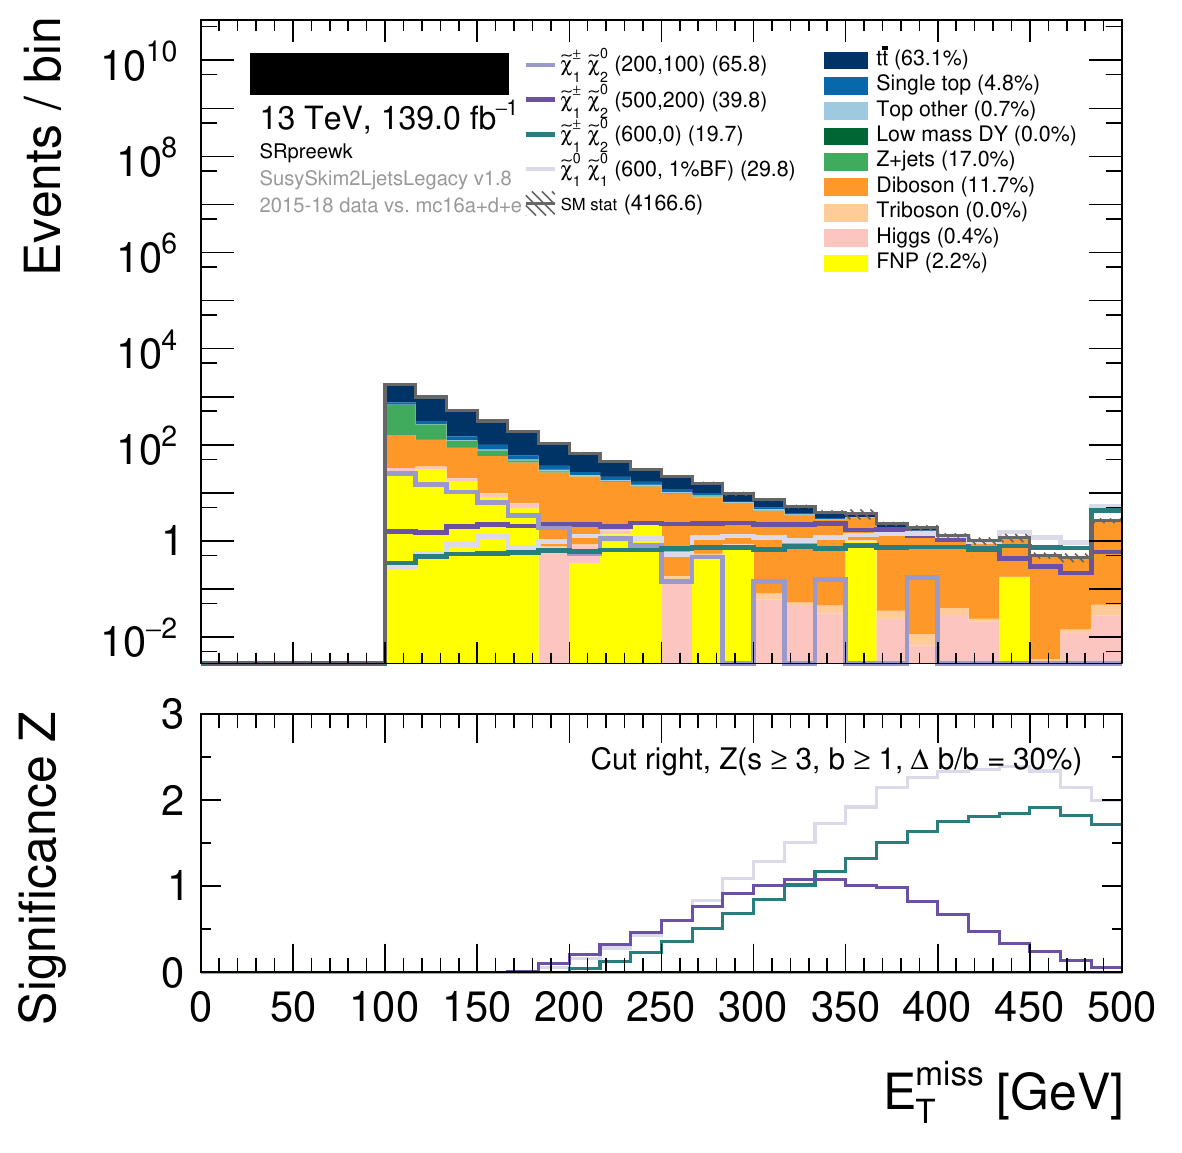
\includegraphics[width=0.48\textwidth]{figures/2ljets_presel_met_logy.png}
\hfill
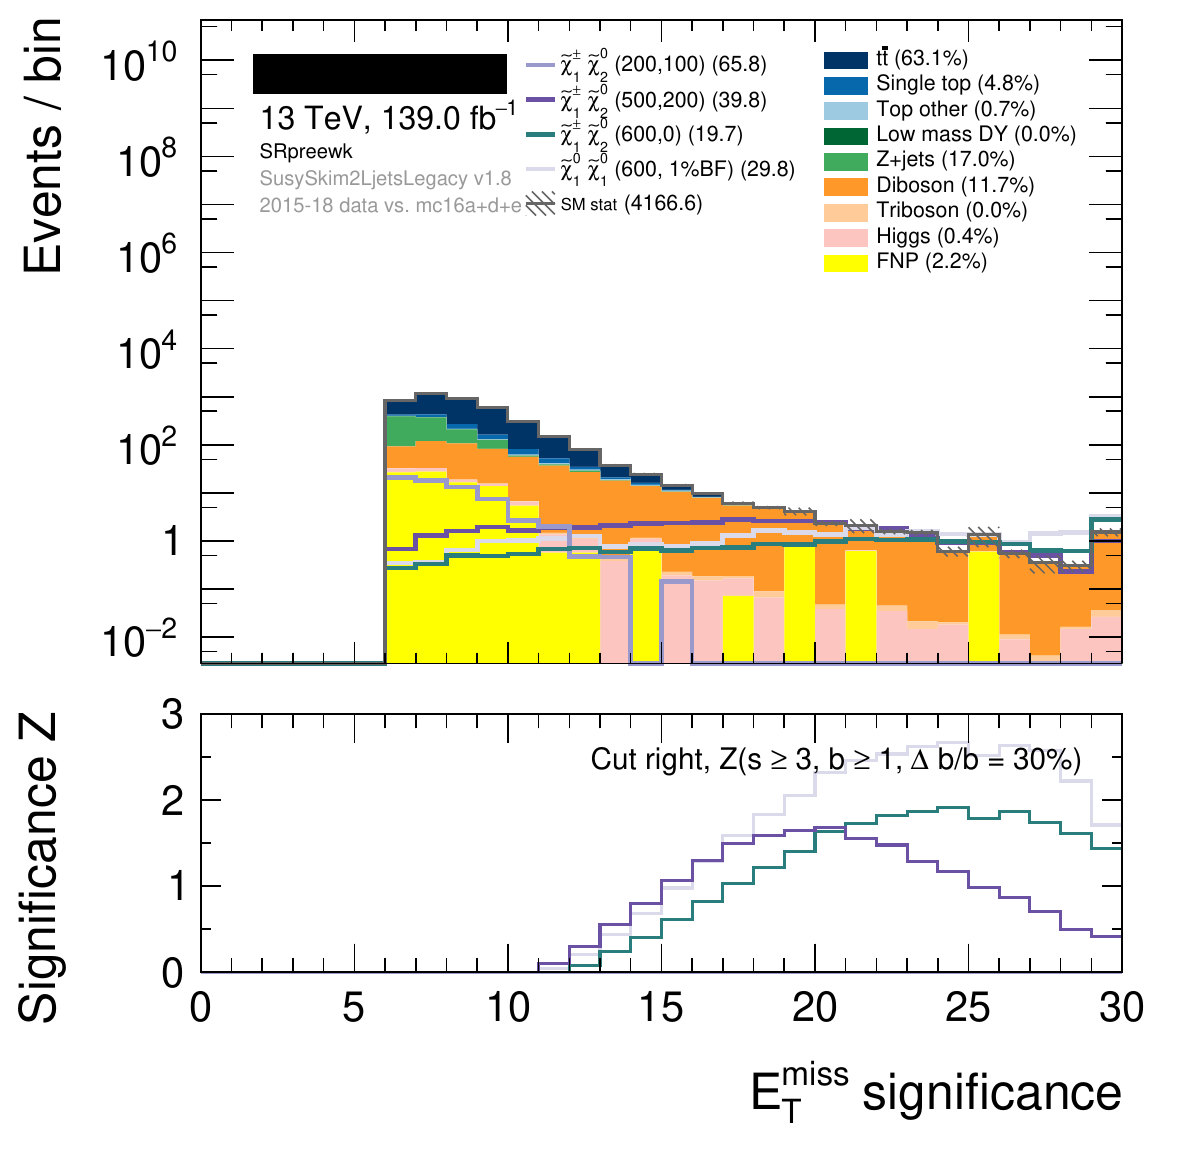
\includegraphics[width=0.48\textwidth]{figures/2ljets_presel_met_sig_logy.png}
\caption[
Illustration of how $\metsig$ beats $\met$ in sensitivity to example signal
models
]{
Illustration of how $\metsig$ beats $\met$ in sensitivity to example signal
models.
At large $\metsig$, $\ttbar$ and other backgrounds are suppressed, leaving
quite pure diboson backgrounds and greater significance measures.
Signal models with smaller mass-splittings tend to have the bulk of their
events at smaller $\met$.
\\[0.5em]
This selection requires two same-flavour opposite-sign signal leptons with
$\pt^{\ell_2} > 25\,\eV[G]$,
$\mll \in (71, 111)\,\eV[G]$,
$\mjj \in (60, 110)\,\eV[G]$,
$\nbtag \leq 1$,
$\met > 100\,\eV[G]$, and
$\metsig > 6$.
\\[0.5em]
``Significance'' displayed in the lower subplot uses the Binomial significance
$Z_{Bi}$ from~\cite{cousins2008evaluation}, with a $30\%$ background
uncertainty and yields taken to the right of a given value.
Large values indicate expected sensitivity to the signal model.
}
\label{fig:2ljets_presel_met}
\end{figure}

Uncertainty in $\ptmiss$ is modelled for $\metsig$ by a covariance matrix
$\Sigma$ in the transverse plane, and used to define
\begin{equation}
\metsig^2
=
\ptmiss \Sigma^{-1} \ptmiss
=
\frac{(\met)^2}{\sigma_L^2(1 - \rho_{LT}^2)}
,
\end{equation}
in which $\sigma_L^2$ is the variance in the direction of $\ptmiss$ and
$\rho_{LT}$ is the correlation coefficient between the parallel and
perpendicular components~\cite{atlas_met_significance}.
This is the square of a Mahalanobis (standard-deviations) distance between
the origin and $\ptmiss$~\cite{mahalanobis1936generalised}.

Just as $\ptmiss$ is constructed from a (negative) sum of contributions from
objects in an event,
$\Sigma$ is a sum of covariances assigned to those objects;
both means and variances add linearly.


\subsection{\texorpdfstring{$\mttwo$}{mT2}}
\label{sec:2ljets_mt2}
Just as the slepton is a supersymmetric partner to a lepton, the `stransverse'
mass $\mttwo$ is a partner to the `transverse mass' $m_T$
(to be defined shortly),
that is useful in searches for supersymmetric particles.

The stransverse mass of an event is a greatest lower bound on the mass of a
pair-produced resonance, that applies when each partner decays semi-invisibly.
For example, an on-shell $\tilde\ell^+\tilde\ell^-$ pair decaying as
$\tilde\ell^+ \rightarrow \ell^+ \neutralino_1
,~
\tilde\ell^- \rightarrow \ell^- \neutralino_1$ has
$\mttwo(\ell^+, \ell^-, m(\neutralino_1)) \leq m(\tilde\ell)$, plus some error
margin for experimental resolution.
Such cases are common, since R-parity conservation implies pair production,
and the idea that dark matter could comprise the lightest supersymmetric
particle motivates invisible decays.

Lacking direct observation of sleptons, $\mttwo$ remains useful in separating
standard model processes; dileptonic $\ttbar$ and $W^\pm W^\mp$ decays both
satisfy $\mttwo(\ell^+, \ell^-, 0) \leq m(W)$ (since $0 \approx m(\nu)$).
The $\twoljets$-electroweak search depends on this effect;
most selections require $\mttwo(\ell^+, \ell^-, 0) > 80\,\eV[G]$, or similar,
to reduce $\ttbar$, $W^\pm W^\mp$ and $\tau^\pm\tau^\mp$ backgrounds.

To be precise, the stransverse mass explores how to split the observed
$\ptmiss$ between the two visible decay products in an event, and can be
defined as
\begin{equation}
\mttwo(a_\mu, b_\mu, m)
=
\min_{\vec p + \vec q=\ptmiss}
\max
\begin{Bmatrix}
m_T(a_\mu + \{\!\sqrt{m^2 - \vec p_T^{\:2}},\,\vec p\,\}_\mu)\\
m_T(b_\mu + \{\!\sqrt{m^2 - \vec q_T^{\:2}},\,\vec q\,\}_\mu)\\
\end{Bmatrix}
,
\end{equation}
in which $m_T^2(p_\mu) = p_0^2 - p_1^2 - p_2^2$ and $\{E,\,\vec p\,\}_\mu$ denotes
the four-vector with energy $E$ and momentum $\vec p$~\cite{lester1999measuring}.
As an extension, one can assign different masses $m_p$ and $m_q$ to
the two invisible products~\cite{lester2015bisection}.

Numerical evaluation of $\mttwo$ can be performed efficiently with interval
bisection algorithms, which seek the least resonance mass for which the
transverse masses allow any compatible assignment which also satisfies
$\vec p + \vec q = \ptmiss$.
Testing this compatibility reduces to testing for the intersection of two
ellipses, one for each transverse
mass~\cite{cheng2008minimal, lester2015bisection}.

Public code for calculating $\mttwo$ is available in a Python
library~\cite{gillam2021mt2}, to which I contributed a faster and more robust
implementation of the bisection algorithm by
Lester and Nachman~\cite{lester2015bisection} during this project.


\subsection{Jet pairs}
Di-jet assignments, for variables like $\mjj$ and $\rjj$, are always chosen as
the two hardest jets.
Why?

This choice matches the convention of SR2-int and SR2-high from the previous
search~\cite{atlas_23l_SUSY_2016_24}, but my initial reaction was that since we
are looking for jet pairs near to $m(W)$ or $m(Z)$, we should surely choose
candidate jet pairs by their mass.

Two alternative di-jet assignments were therefore considered in early
development of region designs:
the two jets with invariant mass closest to $m(W)$, and the two jets with the
minimum $\rjj^\mathrm{alternative}$ between them.
The result was bland.
All assignments performed similarly, and all left similar fractions of signal
yields outside the mass window.
The simplicity and precedent for the two-hardest jet assignment therefore swung
the decision.

However, alternatives did select different subsets of signal yields;
the alternative jet assignments had some potential to define secondary signal
regions to catch those signal events which fall outside the primary
$\mjj$ window.
One can, for example, select $\mjj \notin 60\textrm{--}110\,\eV[G]$ and
$\mjj^\mathrm{alternative} \in 60\textrm{--}110\,\eV[G]$ for some additional
sensitivity.
However, this comes at the cost of complexity, particularly in the boundaries
with control and validation regions, and is therefore not used here.


\subsection{Cheat-sheet}
Uncomfortably many event variables are used to define the regions of this
analysis.
To aid future revision of their meanings, definitions, and references for these
variables are collected here.
All dimensionful quantities are in $\eV[G]$.
\begin{itemize}
\item $\met$: missing transverse momentum
\item $\metsig$: object-based missing transverse momentum significance;\\
described in Section~\ref{sec:2ljets_metsig}
\item $\ptjone$: transverse momentum of the hardest jet%
\vspace{0.5em}
\item $\mll$: invariant mass of the hardest two leptons
\item $\mjj$: invariant mass of the two hardest jets
\item $\mbb$: invariant mass of the two hardest $b$-tagged jets
\item $\mjetone$: mass of the hardest jet
\item $\mttwoll$: `stransverse' mass of the lepton pair with massless invisibles;\\
described in Section~\ref{sec:2ljets_mt2}
\vspace{0.5em}
\item $\rll$: distance in $\eta\textrm{--}\phi$ between the lepton pair
\item $\rjj$: distance in $\eta\textrm{--}\phi$ between the two hardest jets%
\vspace{0.5em}
\item $\njet$: number of signal jets
\item $\nbtag$: number of b-tagged jets;
described in Section~\ref{sec:2ljets_btagging}
\vspace{0.5em}
\item $\dphillmet$: azimuthal angle between the lepton pair and $\ptmiss$
\item $\dphijmet$: azimuthal angle between the hardest jet and $\ptmiss$
\end{itemize}
All of these are physical properties of particles or collections of particles.
Please remember that none is an exact or true value;
all are estimates based on approximate reconstructions.
While this distinction is easy to drop in lax language, it is necessary to
understand the shapes of noisy variables such as $\mjj$ and indeed the
existence of $\metsig$.


\FloatBarrier
\section{Design}
Perhaps the most impactful decision in a search is the design of its regions.
Like most decision, these designs must be made to balance conflicting and
vaguely-specified desires, and are informed with incomplete information.

This section describes the designs and rationales behind the control,
validation and signal regions of the $\twoljets$ analysis.

\begin{figure}[tp]
\centering
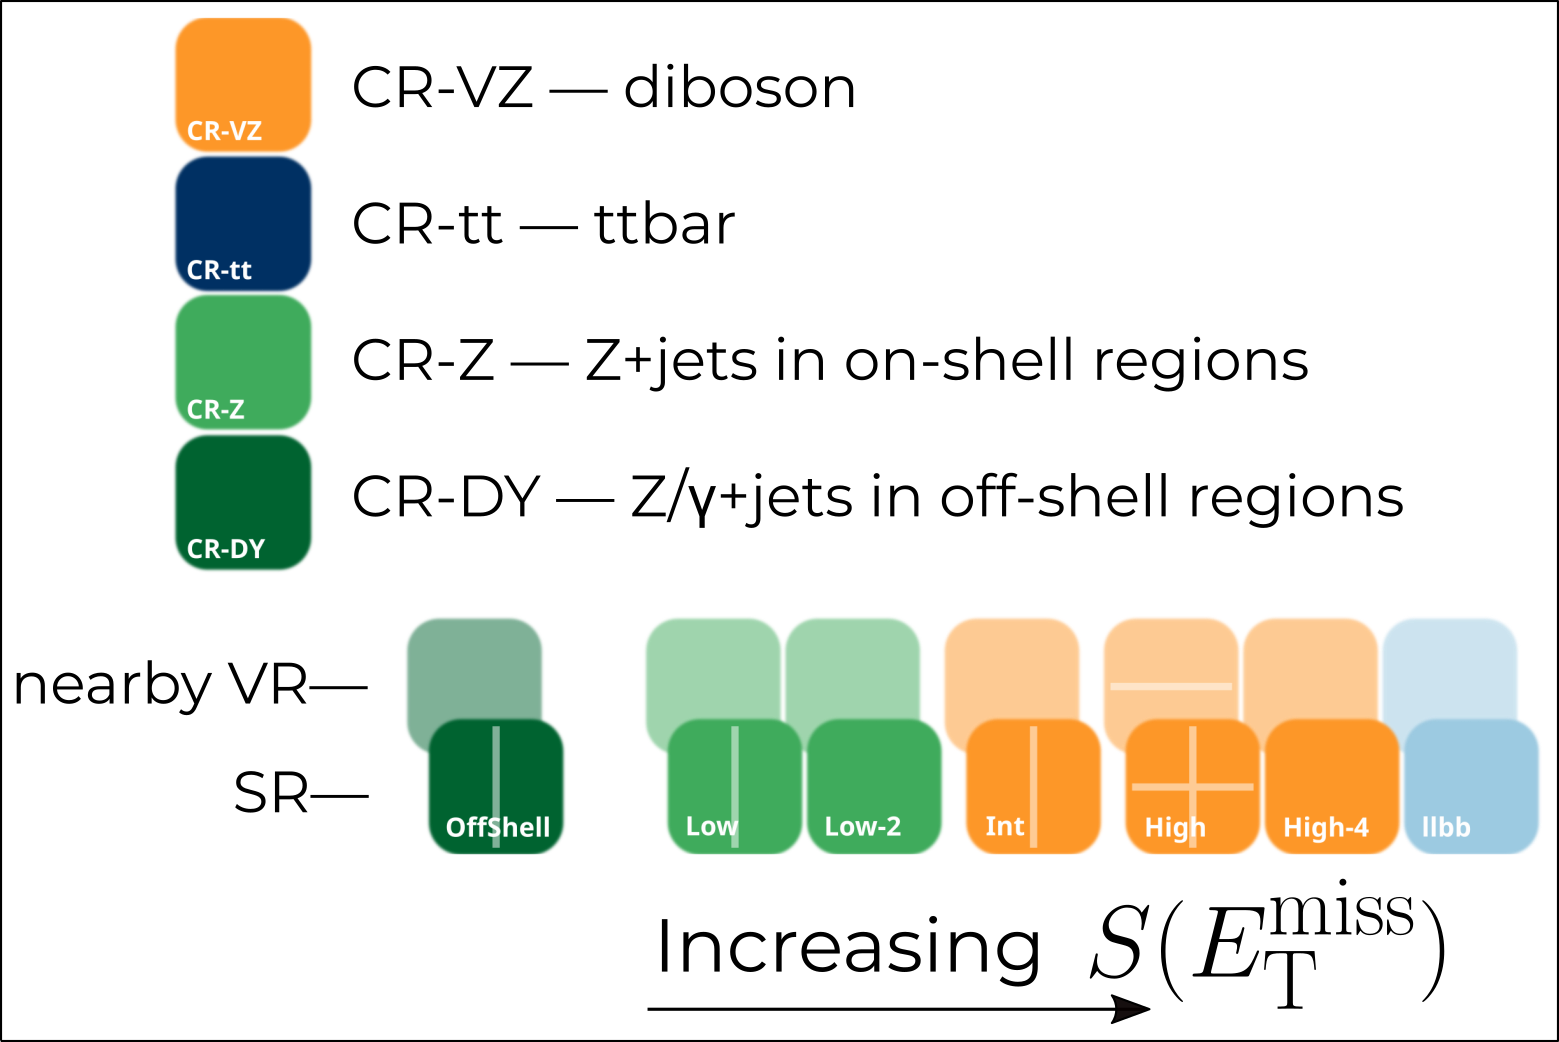
\includegraphics[width=0.99\textwidth]{figures/2Ljets_pam_ewkslide.png}
\caption[
Region design summary slide
]{%
Region design summary slide adapted from an internal presentation.
Colours represent primary background contributions in our plotting scheme.
}
\label{fig:2ljets_region_summary}
\end{figure}

The clearest idea behind this design is to split regions on $\metsig$.
Motivation for this design is displayed in
Figure~\ref{fig:2ljets_presel_met};
$\metsig$ does better than $\met$ in separating background and signal
contributions for models with various mass splittings above $m(Z)$.
Furthermore, $\metsig$ also works to separate signal models from each other;
signals with larger mass differences in their decays to invisibles tend to have
larger $\metsig$.
Binning regions in $\metsig$ therefore also improves sensitivity to
individual parameter points and allows targeted selections on other,
locally-relevant, event variables.

Regions in three blocks of $\metsig$ are named High, Intermediate (or Int),
and Low,
which target models with decreasing mass splittings and lepton pairs on the
$Z$ resonance mass.
Separate regions target $\mll < m(Z)$ for models with small mass splittings,
which force decays to proceed via low-mass off-shell weak bosons.

Following the conventional style descibed in
Section~\ref{sec:searches_searches},
control regions are defined to normalize specific background samples,
and validation regions are defined to test their extrapolation towards
signal regions before unblinding.

All regions are defined within a loose `Pre-selection' requirement which
requires the basic $Z\rightarrow \ell^+\ell^-$ plus jets pluts $\met$
conditions that we target in the $\twoljets$-electroweak.
These Pre-selection requirements are defined in Table~\ref{tab:2ljets_presel}.

\begin{table}[tp]
\centering
\begin{tabular}{c}
Pre-selection:
\\[1em]
$n_\mathrm{leptons}^\mathrm{signal} = n_\mathrm{leptons}^\mathrm{baseline} = 2$
\\[0.5em]
same flavour, opposite charge leptons
\\[0.5em]
$\njet \geq 1$
\\[0.5em]
$p_\mathrm{T}^{\,\ell_2} > 25$
\\[0.5em]
$\metsig > 6$
\\[0.5em]
$\met > 100$
\end{tabular}
\caption[%
Pre-selection requirements ensured prior to all region definitions in the
$\twoljets$-electroweak search
]{%
Pre-selection requirements ensured prior to all region definitions in the
$\twoljets$-electroweak search.
Although $\metsig > 6$ implies that most events already have large $\met$
$\met > 100\,\eV[G]$ requirement is included to ensure that events with small
$\met$ and smaller uncertainties on it are excluded.
}
\label{tab:2ljets_presel}
\end{table}

High regions are discussed in Section~\ref{sec:2ljets_high}.
Intermediate regions are discussed in Section~\ref{sec:2ljets_int}.
Low regions are discussed in Section~\ref{sec:2ljets_low}.
Off-shell regions are discussed in Section~\ref{sec:2ljets_high}.
Control and validation regions are included in these sections near to their
targetted regions.
Finally, how these are combined into `Discovery' regions for
model-independent interpretations is discussed in
Section~\ref{sec:2ljets_disco}.

A high-level summary of the region design is shown in
Figure~\ref{fig:2ljets_region_summary}.
The design comprises four control regions and thirteen orthogonal signal region
bins, with validation regions targeting each group of signal regions.


% presel table should come before High
\FloatBarrier
\subsection{High}
\label{sec:2ljets_high}
The highest $\metsig$ selections, of around $\metsig > 18$, contain almost pure
diboson backgrounds in relatively small quantities, along with the bulk masses
of signal samples at the heaviest resonance masses.
This is therefore the most promising territory for signal regions which are
highly sensitive to the most extreme signals.
Their backgrounds, however, must be constrained by control regions in less
extreme parameter spaces with more data.

Diboson backgrounds and C1N2 signals have more in common than just $\met$.
Notably, both also produce resonant $Z\rightarrow \ell^+\ell^-$ pairs
and do not enhance the rate of heavy-flavour jets, as displayed in
Figure~\ref{fig:2ljets_high_mll_b}.
Since signals and backgrounds have such similar shapes in $\mll$ and $\nbtag$,
sensitivity is only decreased by rejecting portions of these distributions.
Although most $\twoljets$-electroweak regions use tighter selection on these
variables to reduce backgrounds, this observation allows us to win
additional sensitivity in High regions by loose requirements.

The high regions, defined in Table~\ref{tab:2ljets_high}, comprise SR-High,
SR-High-1J, and SR-$\llbb$.

\begin{table}[tp]
\centering
\begin{tabular}{lccccc}
& $\njet$
& $\nbtag$
& $\metsig$
& $m_*$
& $\rjj$
\\[1em]
SR-High
& $\geq2$
& $\leq 1$
& $18\textrm{--}21\textrm{--}\infty$
& $\mjj\!:~  60\textrm{--}110$
& $0\textrm{--}0.8\textrm{--}1.6$
\\[0.5em]
\: VR-High
& $\geq2$
& $\leq 1$
& $> 18$
& $\uwave{\mjj\!:~  20\textrm{--}60 \mid 110\textrm{--}\infty}$
& $< 1.6$
\\[0.5em]
\: VR-High-R
& $\geq 2$
& $\leq 1$
& $> 18$
& $\uwave{\mjj\!:~  > 20}$
& $\uwave{> 1.6}$
\\[1em]
SR-High-1J
& $\hphantom{\geq}~1$
& $\leq 1$
& $> 12$
& $\mjetone\!:~  60\textrm{--}110$
&
\\[0.5em]
\: VR-High-1J
& $\hphantom{\geq}~1$
& $\leq 1$
& $> 12$
& $\uwave{\mjetone\!:~  20\textrm{--}60 \mid 110\textrm{--}\infty}$
&
\\[1em]
SR-$\llbb$
& $\geq 2$
& $\geq 2$
& $> 18$
& $\mbb\!:~  60\textrm{--}150$
&
\\[0.5em]
\: VR-$\llbb$
& $\geq 2$
& $\geq 2$
& $\uwave{12\textrm{--}18}$
& $\mbb\!:~  60\textrm{--}150$
&
\end{tabular}
\\[1em]
Common: Pre-selection,
$\mll \in 71\textrm{--}111$, and
$\mttwoll > 80$.
\caption[
High region definitions in the $\twoljets$-electroweak analysis
]{%
High region definitions in the $\twoljets$-electroweak analysis.
En-dashes `$a\textrm{--}b$' indicate open intervals $(a, b)$.
Concatenated intervals `$a\textrm{--}b\textrm{--}c$' indicate binning
with boundaries at $a$, $b$, and $c$.
The mid-bar `$\mid$' indicates logical or.
Differences between regions are \uwave{underlined}.
\\[0.5em]
The $\rll$ bins of SR-High are labelled SR-High-8 and SR-High-16, and their
$\metsig$ binns are suffixed -a and -b for $\metsig \in 18\textrm{--}21$
and $\metsig > 21$ respectively.
}
\label{tab:2ljets_high}
\end{table}

\begin{figure}[tp]
\centering
\begin{subfigure}{0.48\textwidth}
\centering
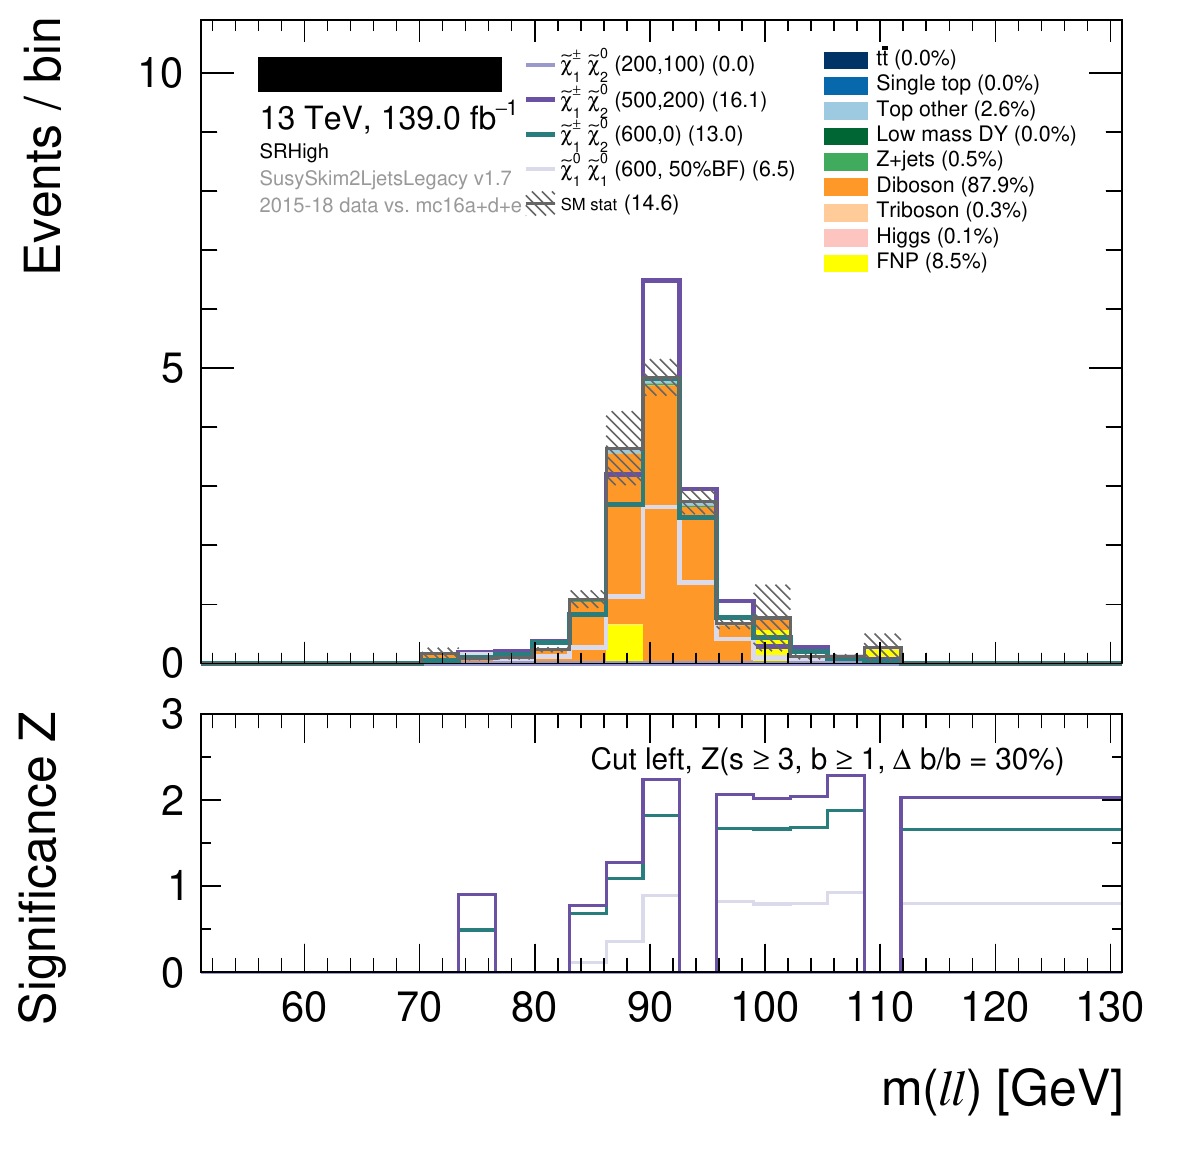
\includegraphics[width=\textwidth]{figures/2ljets_region_design_hist1d_mll_SRHigh.png}
\caption{SR-High, $\mll$}
\end{subfigure}
\hfill
\begin{subfigure}{0.48\textwidth}
\centering
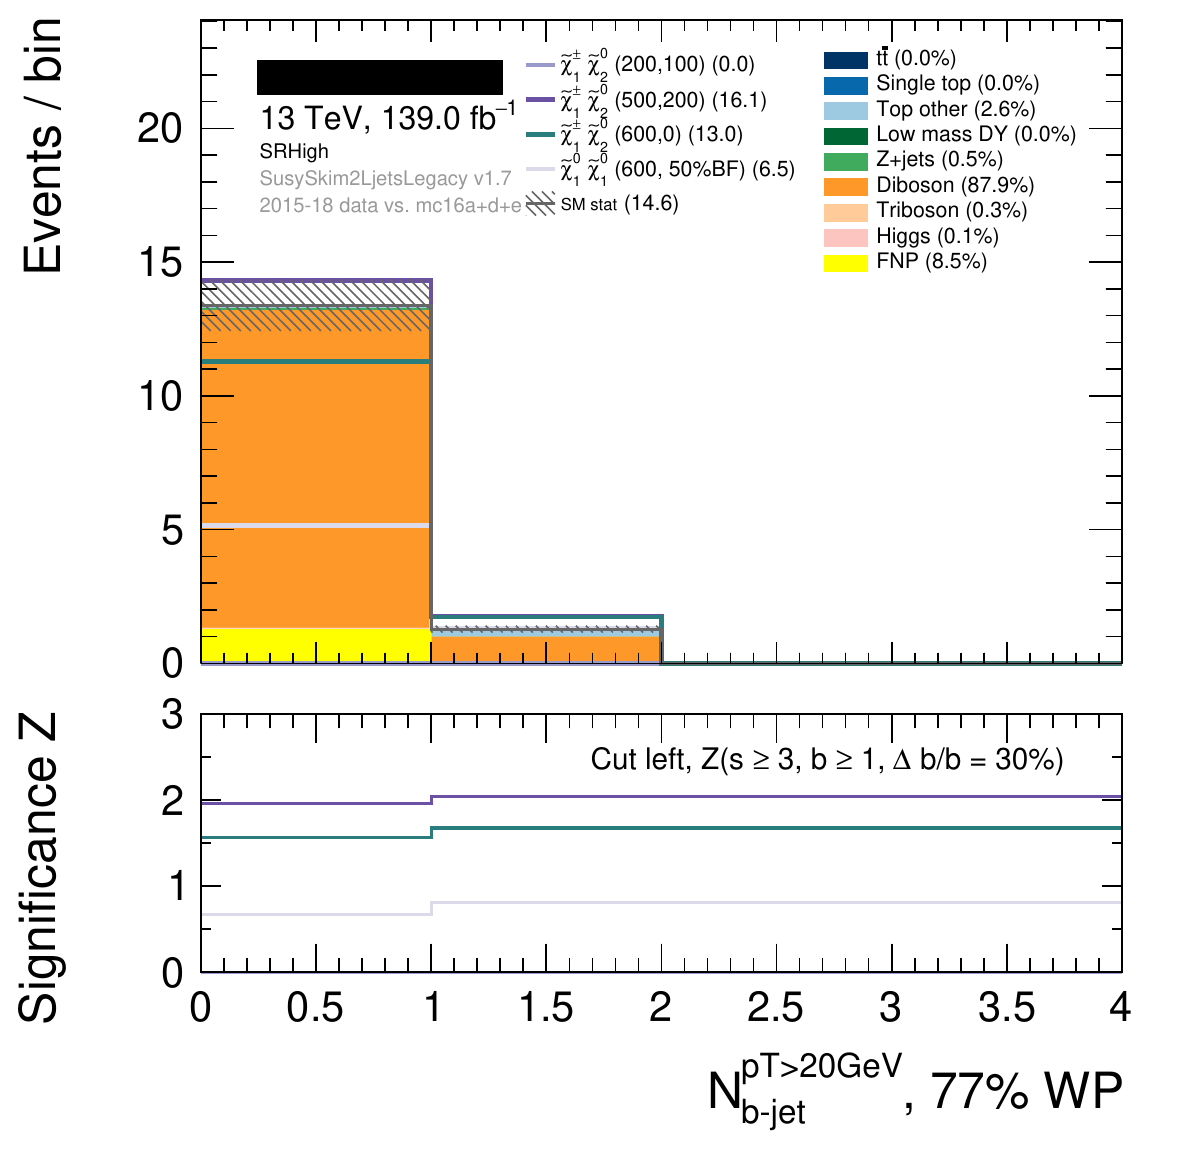
\includegraphics[width=\textwidth]{figures/2ljets_region_design_hist1d_nbtag_SRHigh.png}
\caption{SR-High, $\nbtag$}
\end{subfigure}
\caption[
SR-High with relaxed selections on (a) $\mll$ or (b) $\nbtag$
]{%
SR-High with relaxed selections on (a) $\mll$ or (b) $\nbtag$.
The pure diboson background has very similar shapes to the signals.
Tighter cuts would therefore reduce background and signal yields comparably,
reducing sensitivity.
The significance dropouts in (a) are errors in plotting.
`Significance Z' is the binomial significance with $30\%$ relative background
uncertainty~\cite{cousins2008evaluation}.
Error bars are statistical.
}
\label{fig:2ljets_high_mll_b}
\end{figure}

The $\mll \in 71\textrm{--}111$ window loosely selects the $m(Z)$ peak to
scoop up nearby rare or mismeasured events.
Similarly, allowing up to one $b$-tag improves yields without boosting
backgrounds, since the $\metsig$ requirement already removes most $\ttbar$
processes.

The standard wide $\mjj \in 60\textrm{--}110\,\eV[G]$ requirement captures
both $W\rightarrow jj$ and $Z\rightarrow jj$ for C1N2 and GMSB models
respectively.

As explained in Section~\ref{sec:2ljets_mt2}, requiring $\mttwo$ above $m(W)$
effectively removes $\ttbar$ and other backgrounds.
The relatively low requirement $\mttwoll > 80\,\eV[G]$ is chosen here and
elsewhere in the $\twoljets$-electroweak design to reduce these backgrounds
while minimize lost signal yields.

To maximize projected sensitivity, SR-High is split into four bins with
one split at $\rjj = 0.8$, to form SR-High-8 and SR-High-16, and a second at
$\metsig = 21$ to split these into SR-High-*-a and SR-High-*-b.
For example, SR-High-8-b requires $\rjj < 0.8$ and $\metsig > 21$.
The regions SR-High-8 and SR-High-16 are displayed in
Figure~\ref{fig:2ljets_high_region}, with their -a and -b bins visible across
the $\metsig$ distribution.

\begin{figure}[tp]
\centering
\begin{subfigure}{0.48\textwidth}
\centering
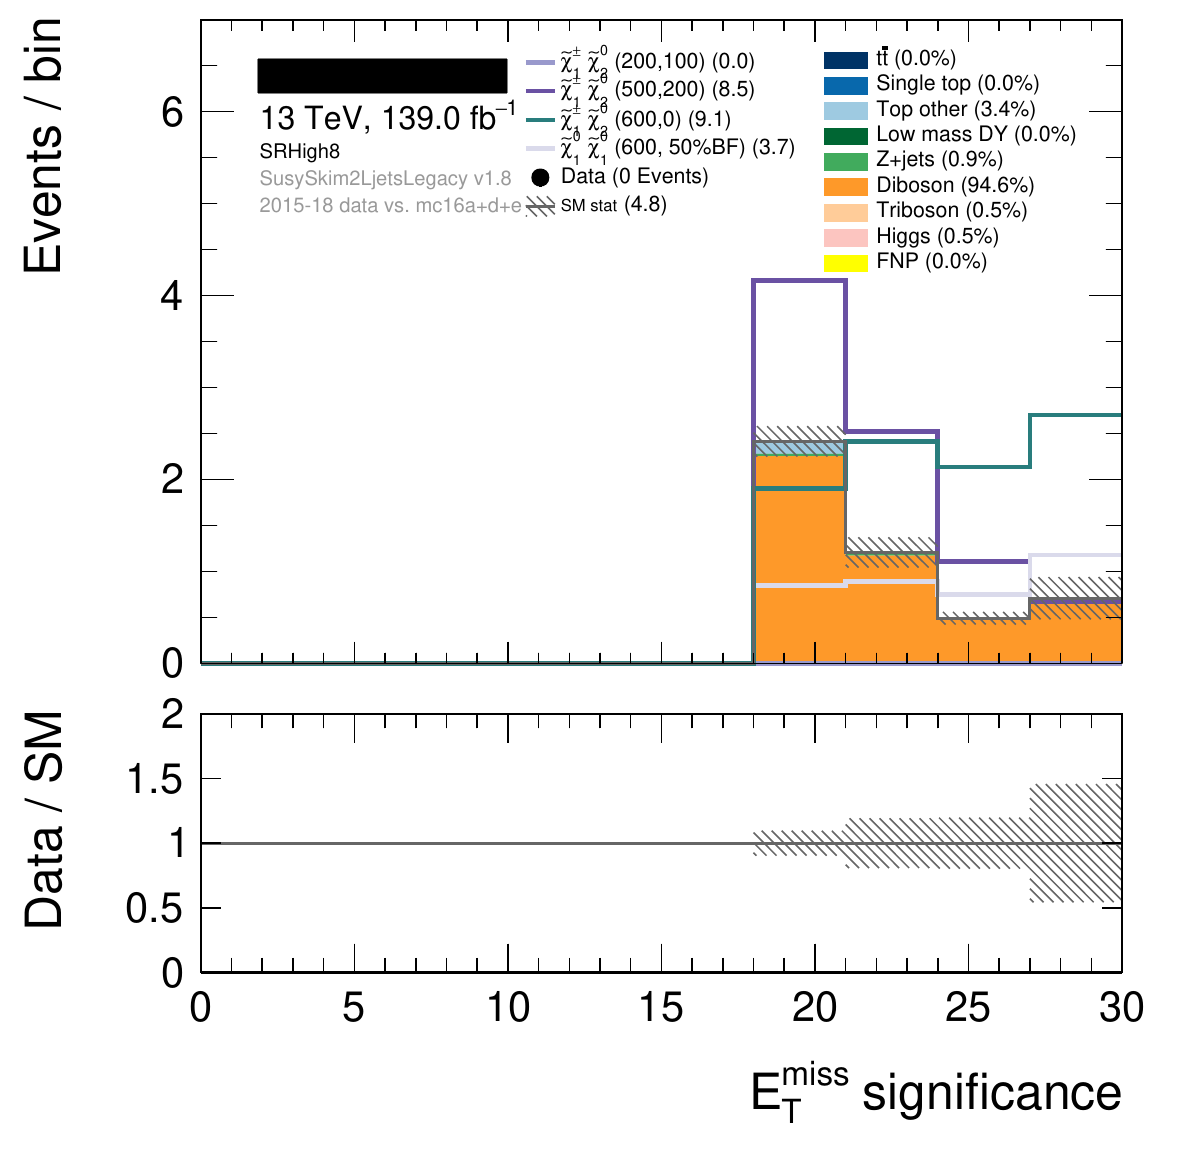
\includegraphics[width=\textwidth]{figures/2ljets_def_met_Sign_SRHigh8.png}
\caption{SR-High-8, $\metsig$}
\end{subfigure}
\hfill
\begin{subfigure}{0.48\textwidth}
\centering
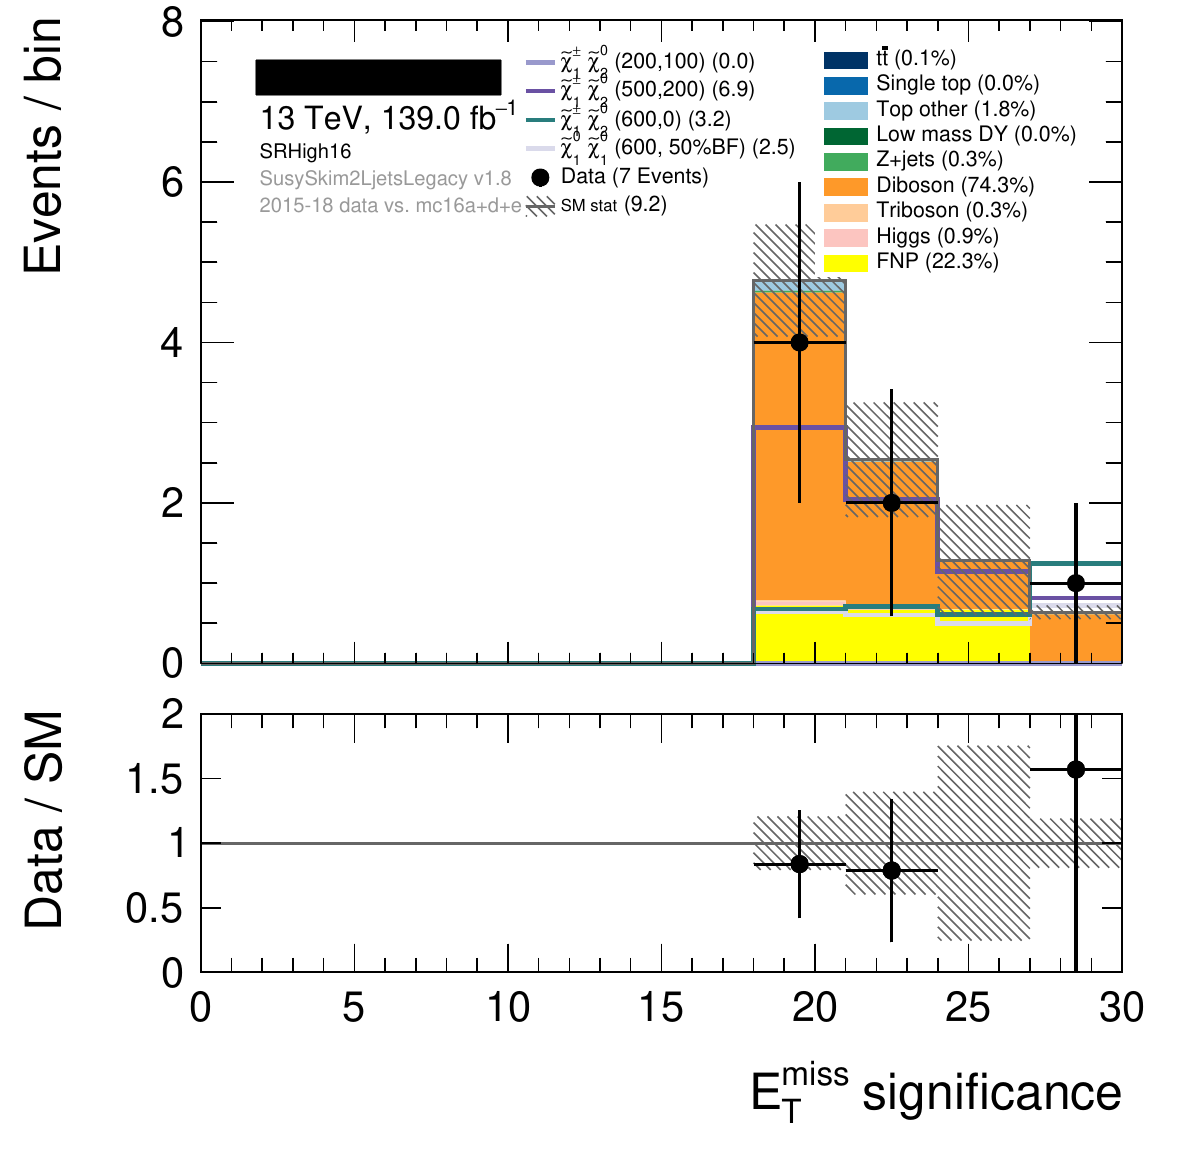
\includegraphics[width=\textwidth]{figures/2ljets_def_met_Sign_SRHigh16.png}
\caption{SR-High-16, $\metsig$}
\end{subfigure}
\\[0.5em]
\begin{subfigure}{0.48\textwidth}
\centering
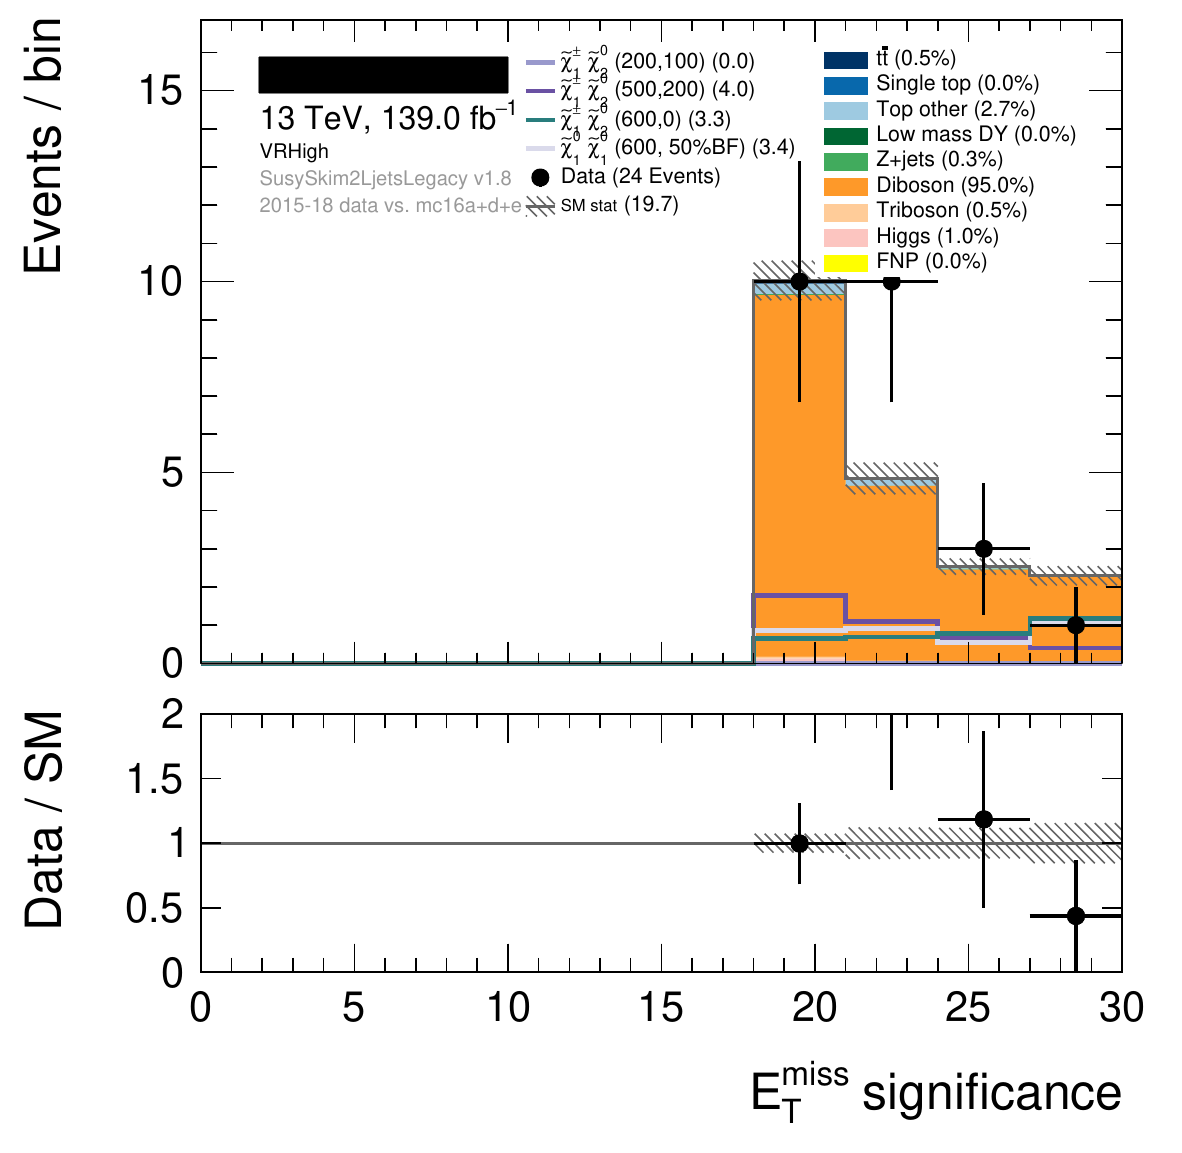
\includegraphics[width=\textwidth]{figures/2ljets_def_met_Sign_VRHigh.png}
\caption{VR-High-8, $\metsig$}
\end{subfigure}
\hfill
\begin{subfigure}{0.48\textwidth}
\centering
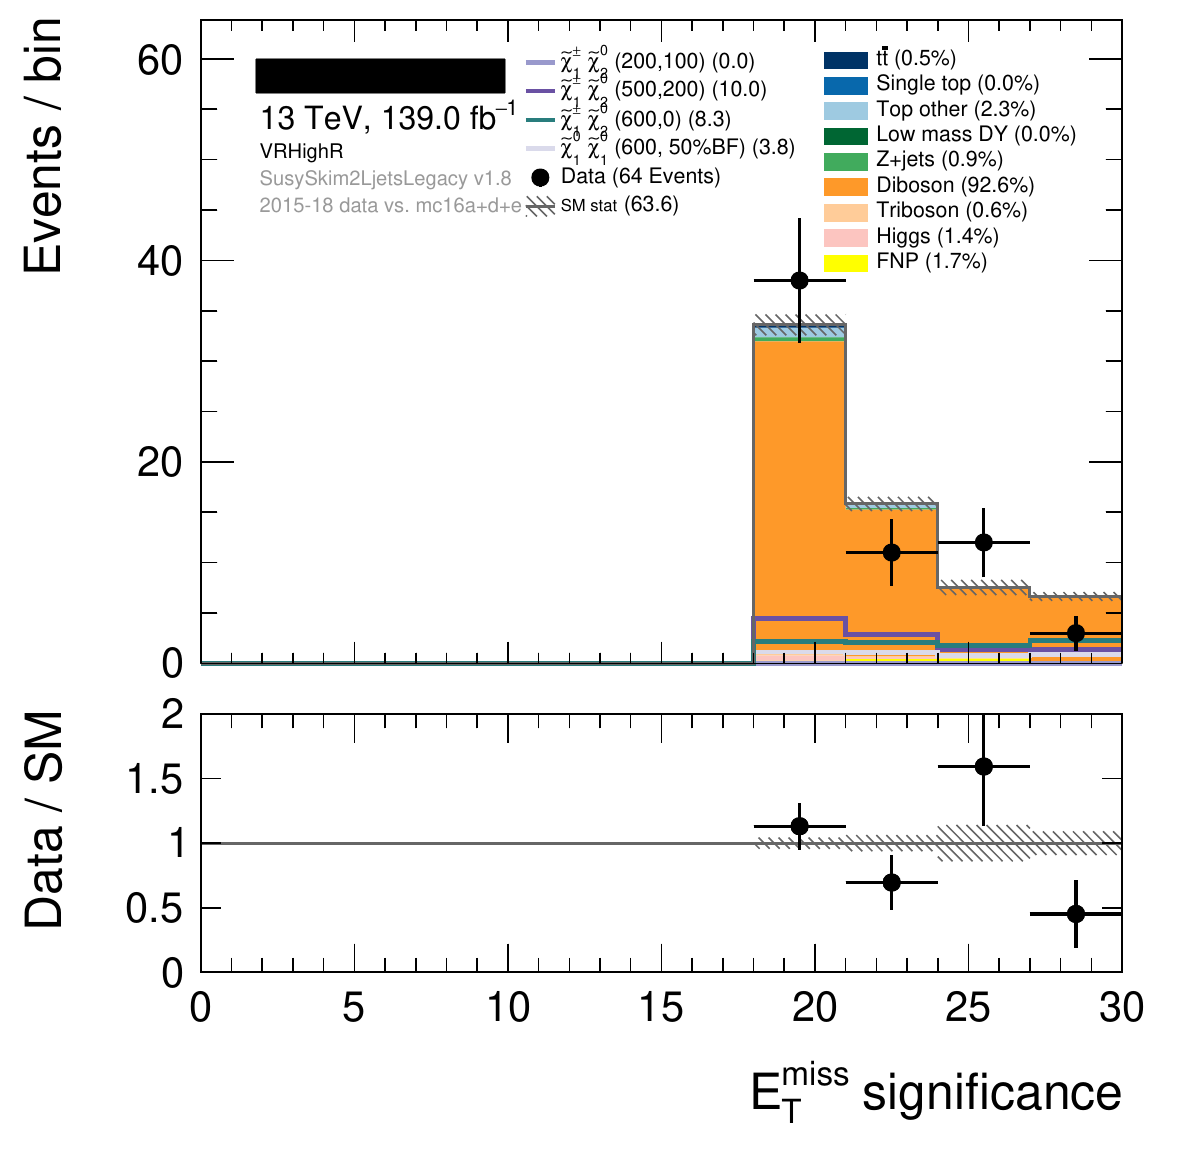
\includegraphics[width=\textwidth]{figures/2ljets_def_met_Sign_VRHighR.png}
\caption{VR-High-16, $\metsig$}
\end{subfigure}
\caption[
Pre-fit distributions of $\metsig$ in High signal and validation regions
]{%
Pre-fit distributions of $\metsig$ in High signal and validation regions.
Signal regions are unblinded.
Errors are statistical.
}
\label{fig:2ljets_high_region}
\end{figure}

One major difference between signals and diboson backgrounds is that signal
jet pairs mostly arise from boosted $W\rightarrow jj$ decays, which more often
produce nearby jets.
Selecting small $\rjj$ in SR-High therefore picks out these boosted cases.

Extremely boosted $W$ bosons can be clustered into single jets.
Although large-radius jets are typically used to capture these, we only use
small, $R=0.4$, jets in the $\twoljets$ analysis.
And those small jets can work for the extreme boosts that our signals produce.
To catch these extreme events is the goal of SR-High-1J, which is displayed
in Figure~\ref{fig:2ljets_high_1J_region}.

\begin{figure}[tp]
\centering
\begin{subfigure}{0.48\textwidth}
\centering
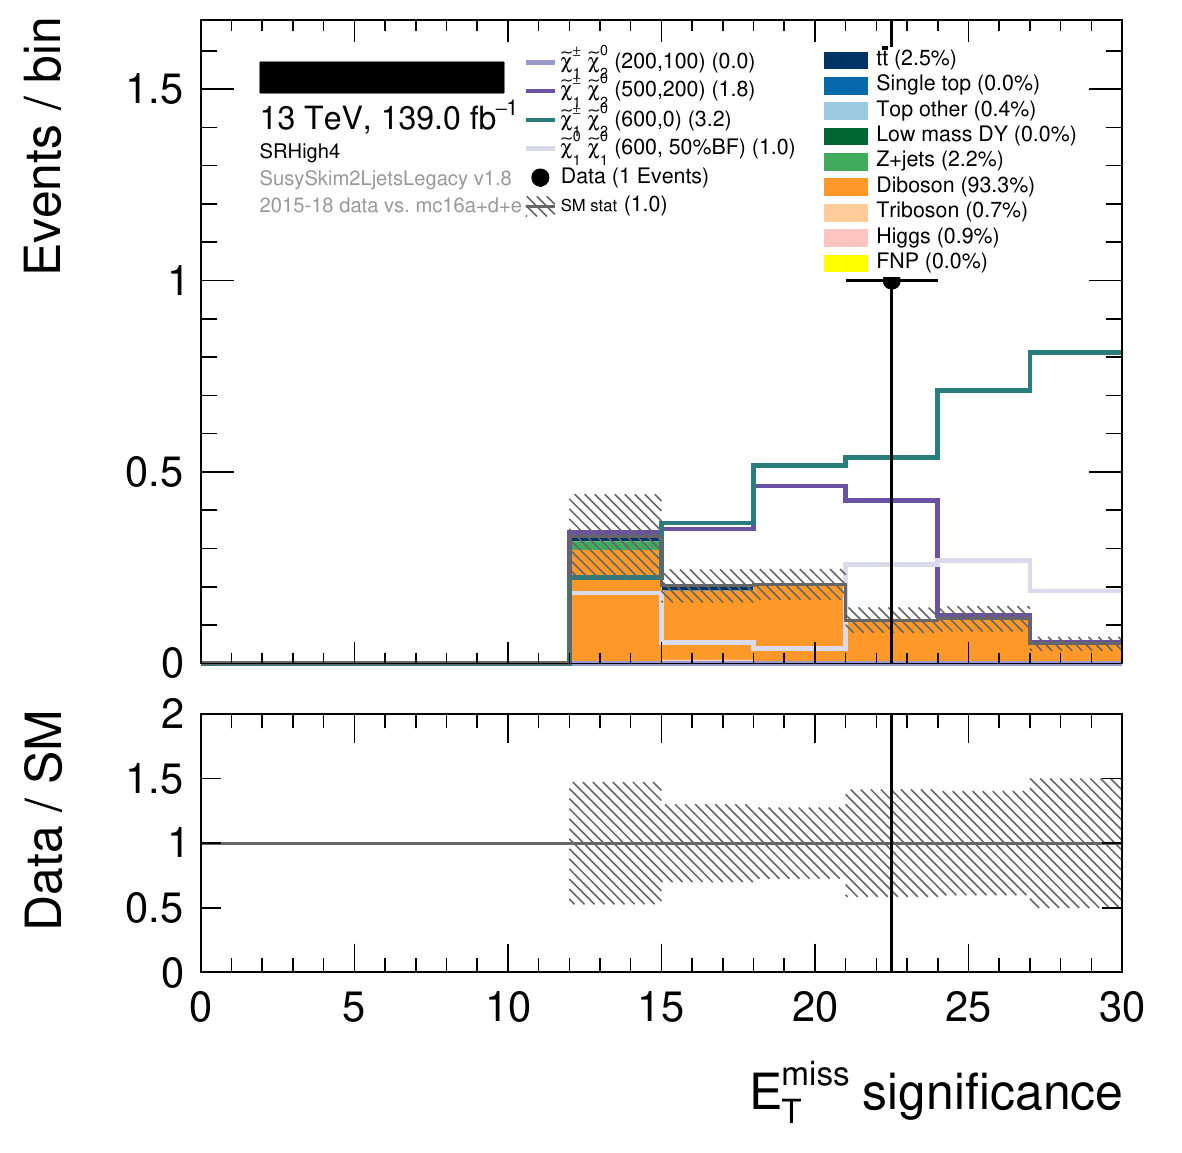
\includegraphics[width=\textwidth]{figures/2ljets_def_met_Sign_SRHigh4.png}
\caption{SR-High-1J, $\metsig$}
\end{subfigure}
\hfill
\begin{subfigure}{0.48\textwidth}
\centering
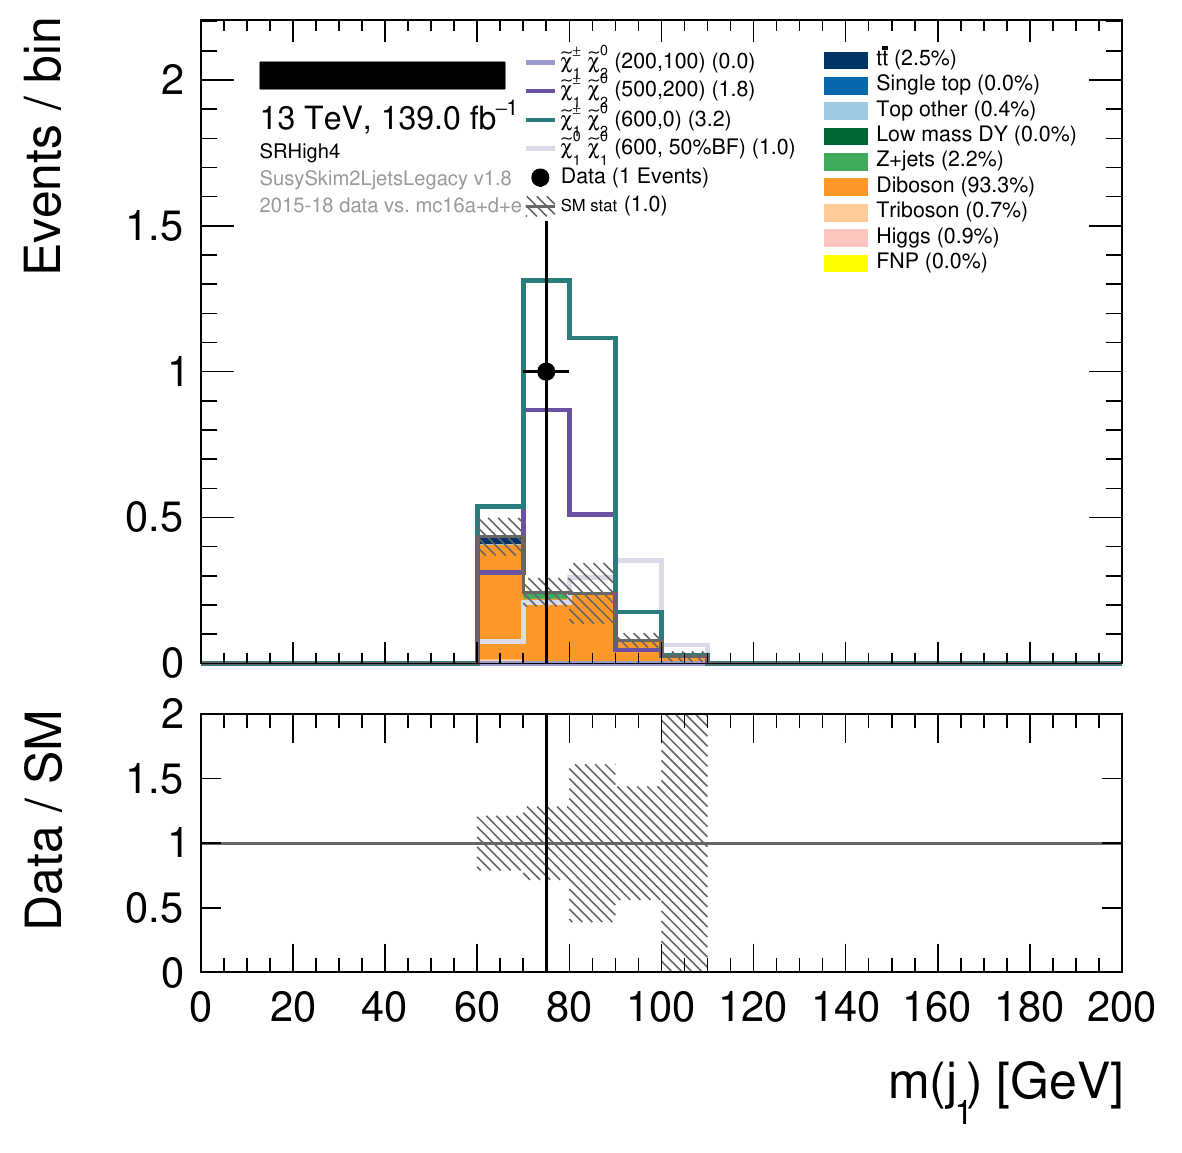
\includegraphics[width=\textwidth]{figures/2ljets_def_mjetone_SRHigh4.png}
\caption{SR-High-1J, $\mjetone$}
\end{subfigure}
\\[0.5em]
\begin{subfigure}{0.48\textwidth}
\centering
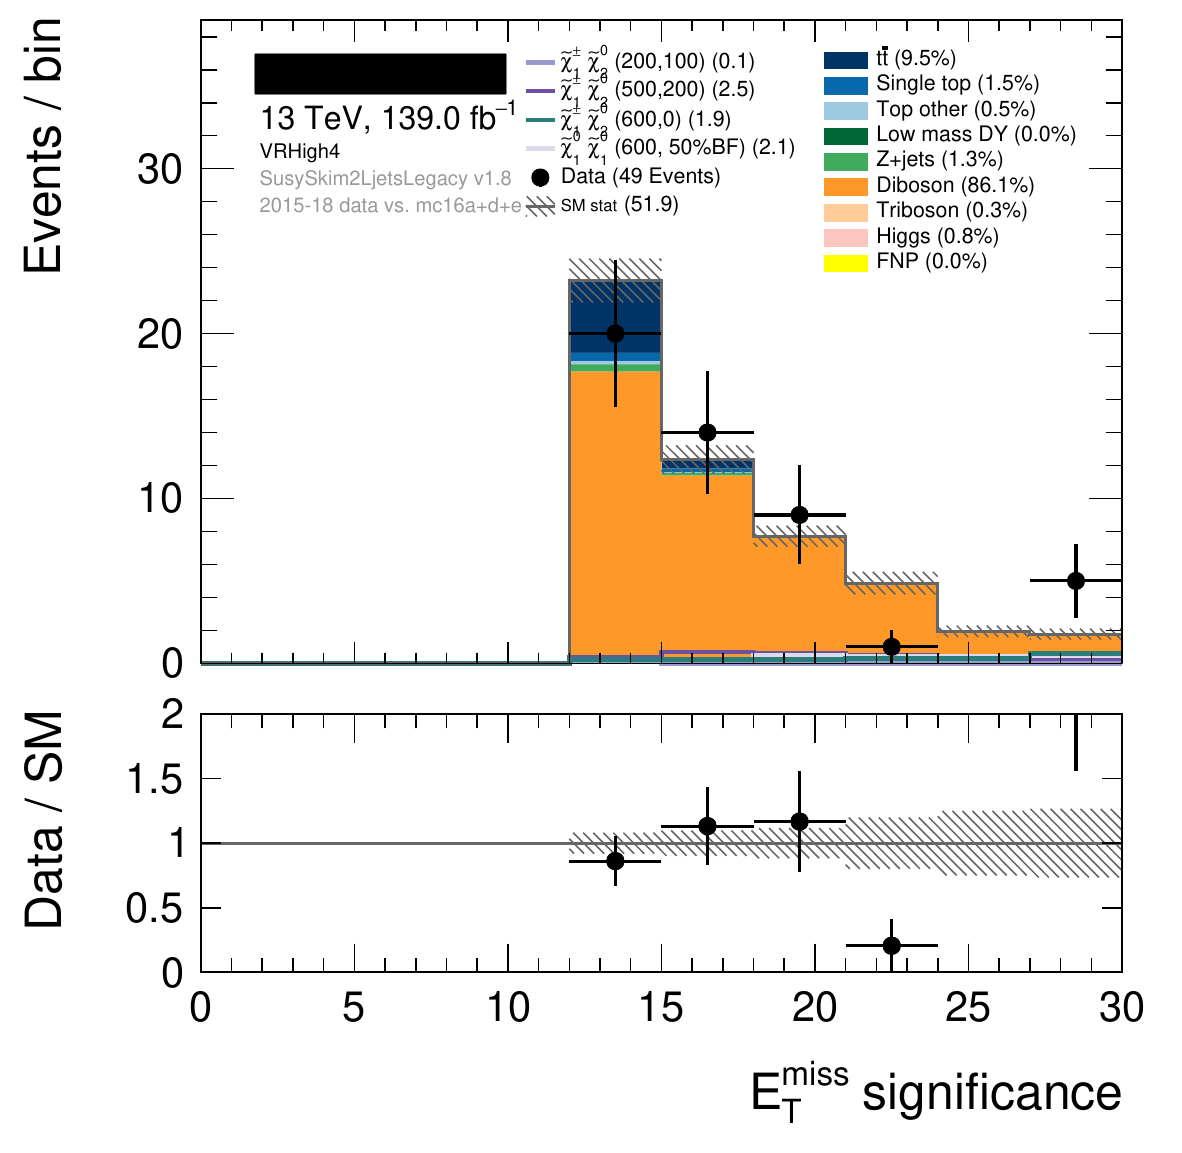
\includegraphics[width=\textwidth]{figures/2ljets_def_met_Sign_VRHigh4.png}
\caption{VR-High-1J, $\metsig$}
\end{subfigure}
\hfill
\begin{subfigure}{0.48\textwidth}
\centering
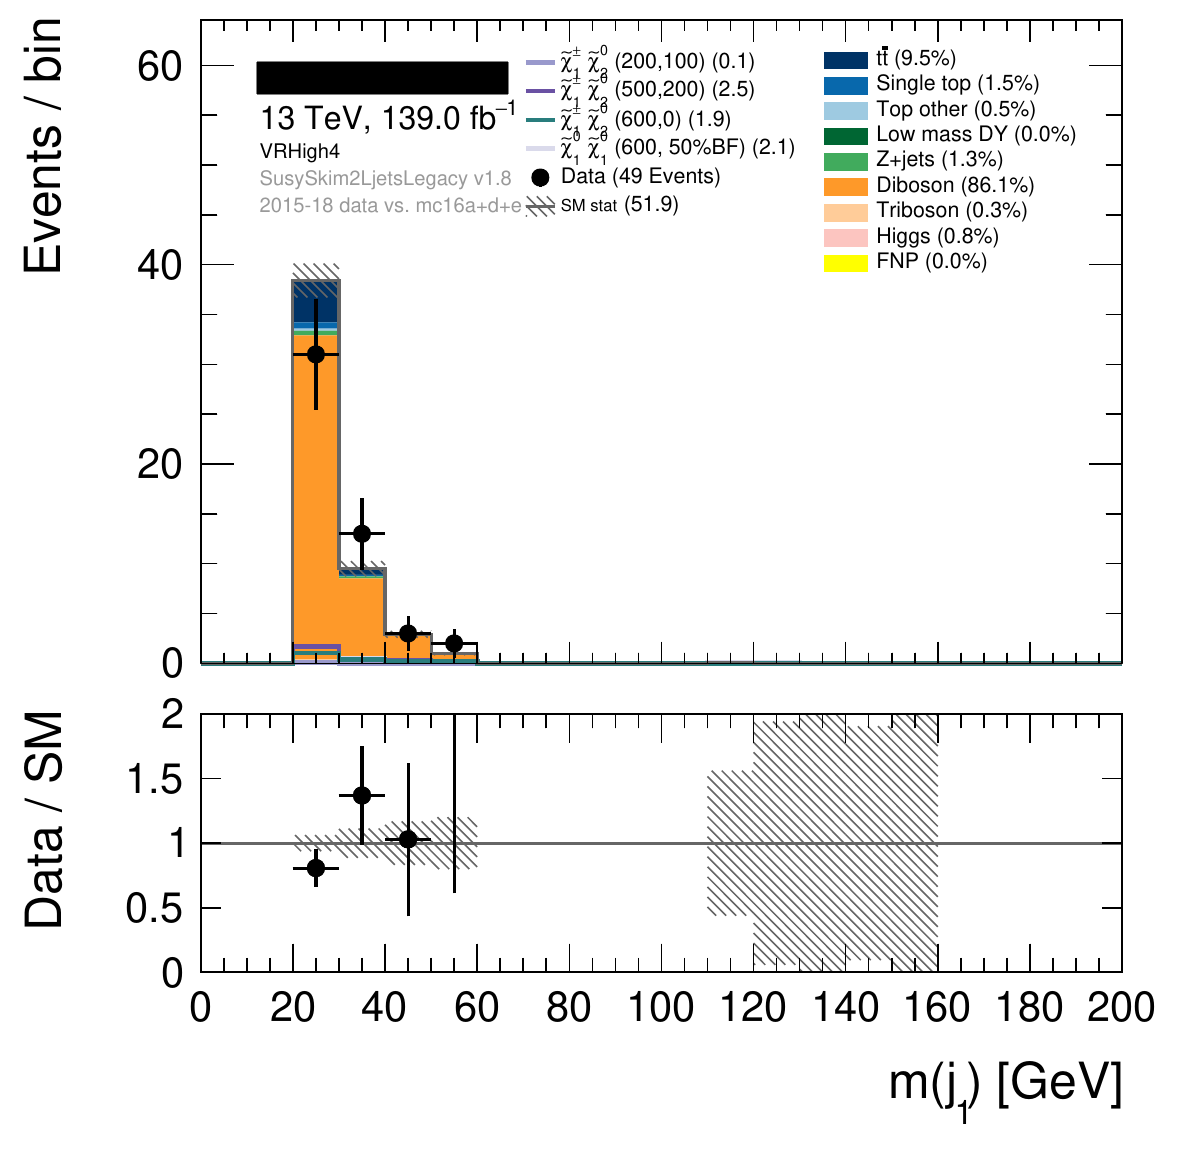
\includegraphics[width=\textwidth]{figures/2ljets_def_mjetone_VRHigh4.png}
\caption{SR-High-1J, $\mjetone$}
\end{subfigure}
\caption[
Pre-fit distributions in mono-jet signal and validation regions
]{%
Pre-fit distributions in mono-jet signal and validation regions.
Signal regions are unblinded.
Errors are statistical.
}
\label{fig:2ljets_high_1J_region}
\end{figure}

All other regions require two jets or more, so this single-jet selection has
the liberty to reduce its $\metsig$ requirement to $\metsig > 12$
without overlapping any other regions.

Finally, SR-$\llbb$ is designed to target the GMSB model, which produces decays
via $ZZ$ and $Zh$ bosons pairs.
Since the $h\rightarrow bb$ branching fraction is large, SR-$\llbb$ finds
sensitivity by requiring a pair of $b$-tagged jets in a heavy mass window.
The low edge of this $\mbb \in 60\textrm{--}150\,\eV[G]$ window is chosen not
only to accommodate \atlas' noisy reconstruction of $b$-jets, but also to
capture $Z\rightarrow bb$ decays, which become significant signal models with
small $B(\neutralino_1 \rightarrow h \gravitino)$.

As shown in Figure~\ref{fig:2ljets_high_llbb_region}, backgrounds in SR-$\llbb$
contain a significant proportion of rare top quark processes;
studies presented in Section~\ref{sec:2ljets_validation} show that these are
mainly $t\bar t Z$.

\begin{figure}[tp]
\centering
\begin{subfigure}{0.48\textwidth}
\centering
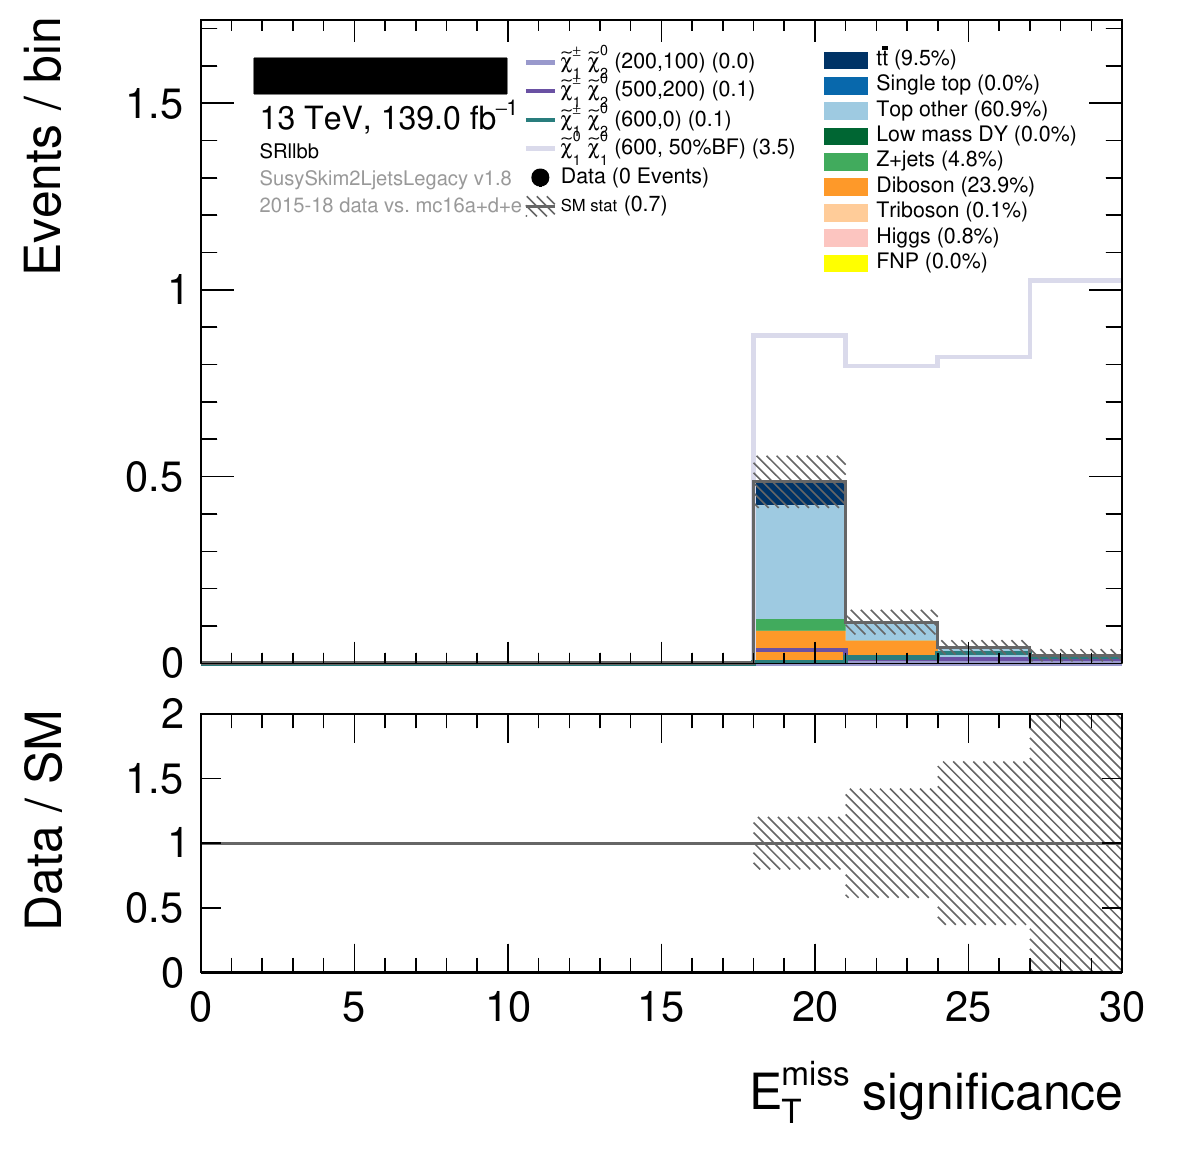
\includegraphics[width=\textwidth]{figures/2ljets_def_met_Sign_SRllbb.png}
\caption{SR-$\llbb$, $\metsig$}
\end{subfigure}
\hfill
\begin{subfigure}{0.48\textwidth}
\centering
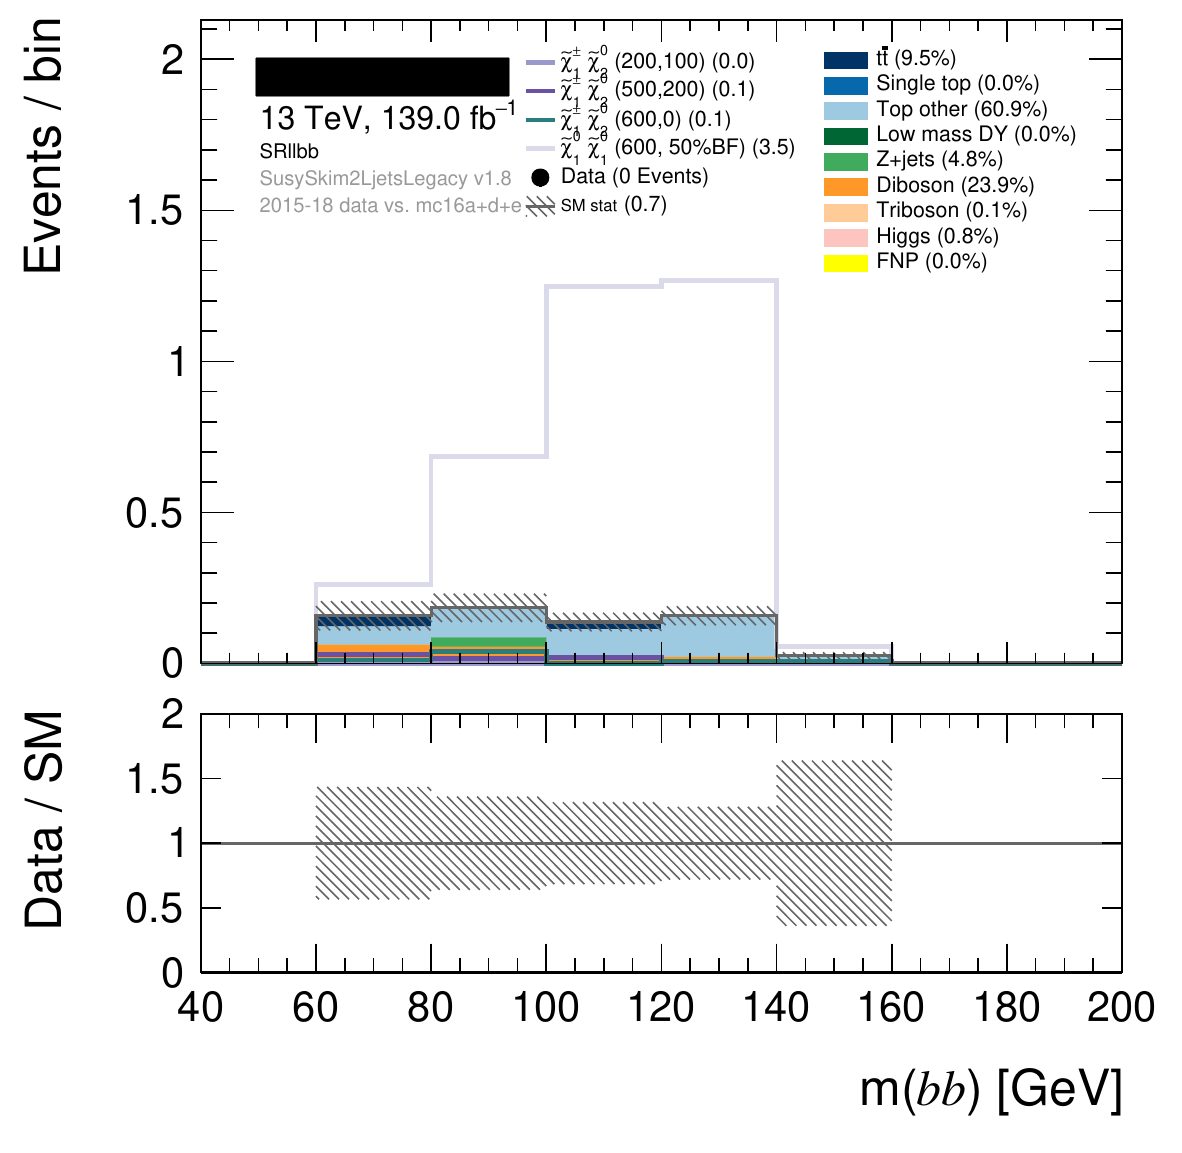
\includegraphics[width=\textwidth]{figures/2ljets_def_mbb_SRllbb.png}
\caption{SR-$\llbb$, $\mbb$}
\end{subfigure}
\\[0.5em]
\begin{subfigure}{0.48\textwidth}
\centering
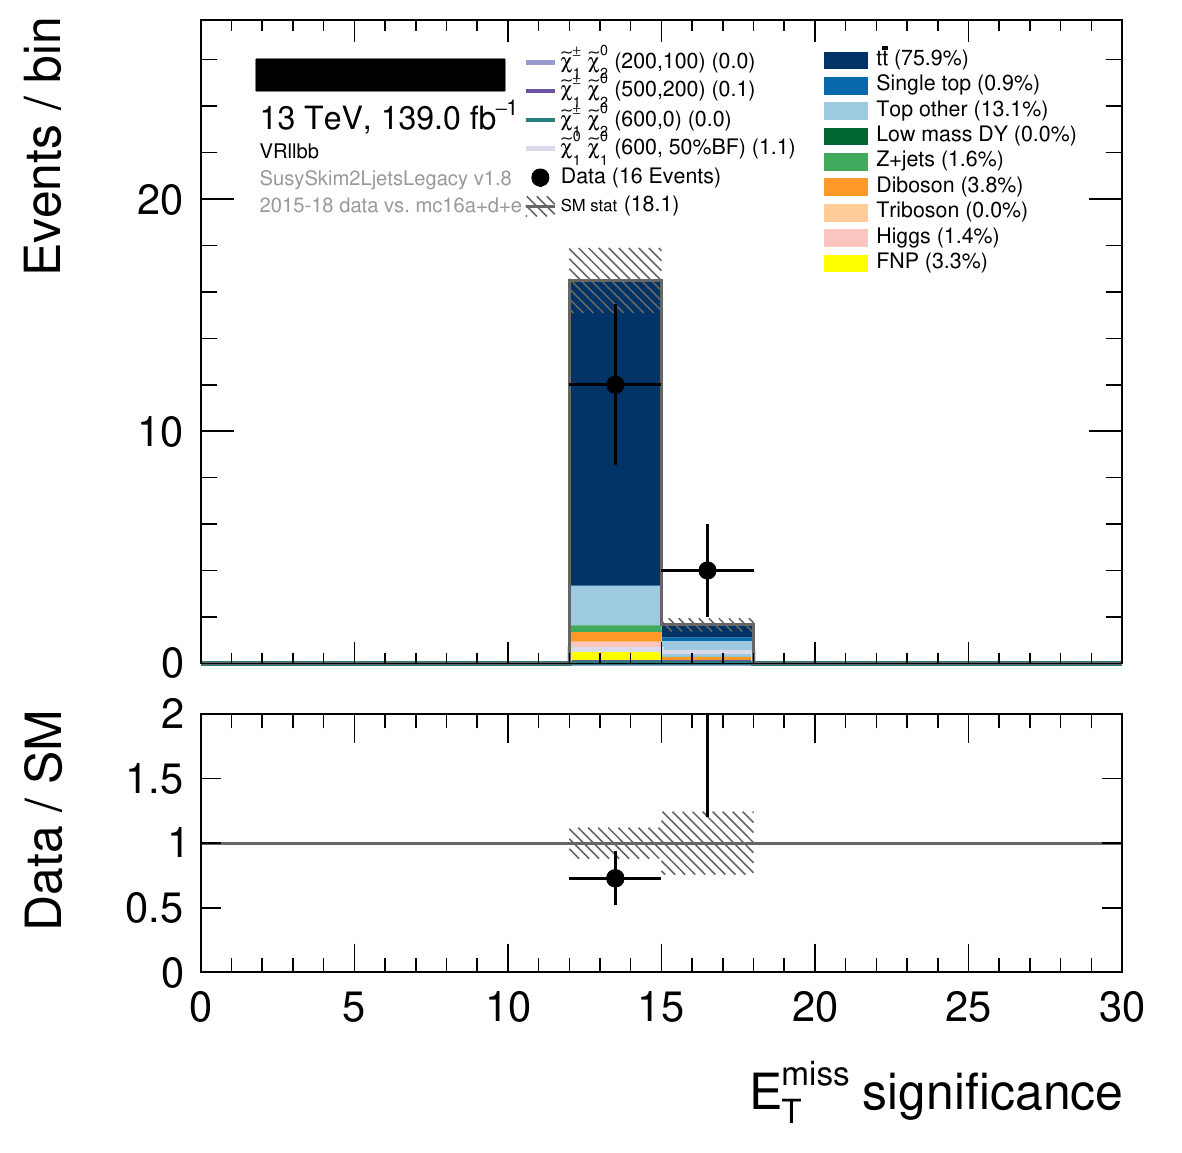
\includegraphics[width=\textwidth]{figures/2ljets_def_met_Sign_VRllbb.png}
\caption{VR-$\llbb$, $\metsig$}
\end{subfigure}
\hfill
\begin{subfigure}{0.48\textwidth}
\centering
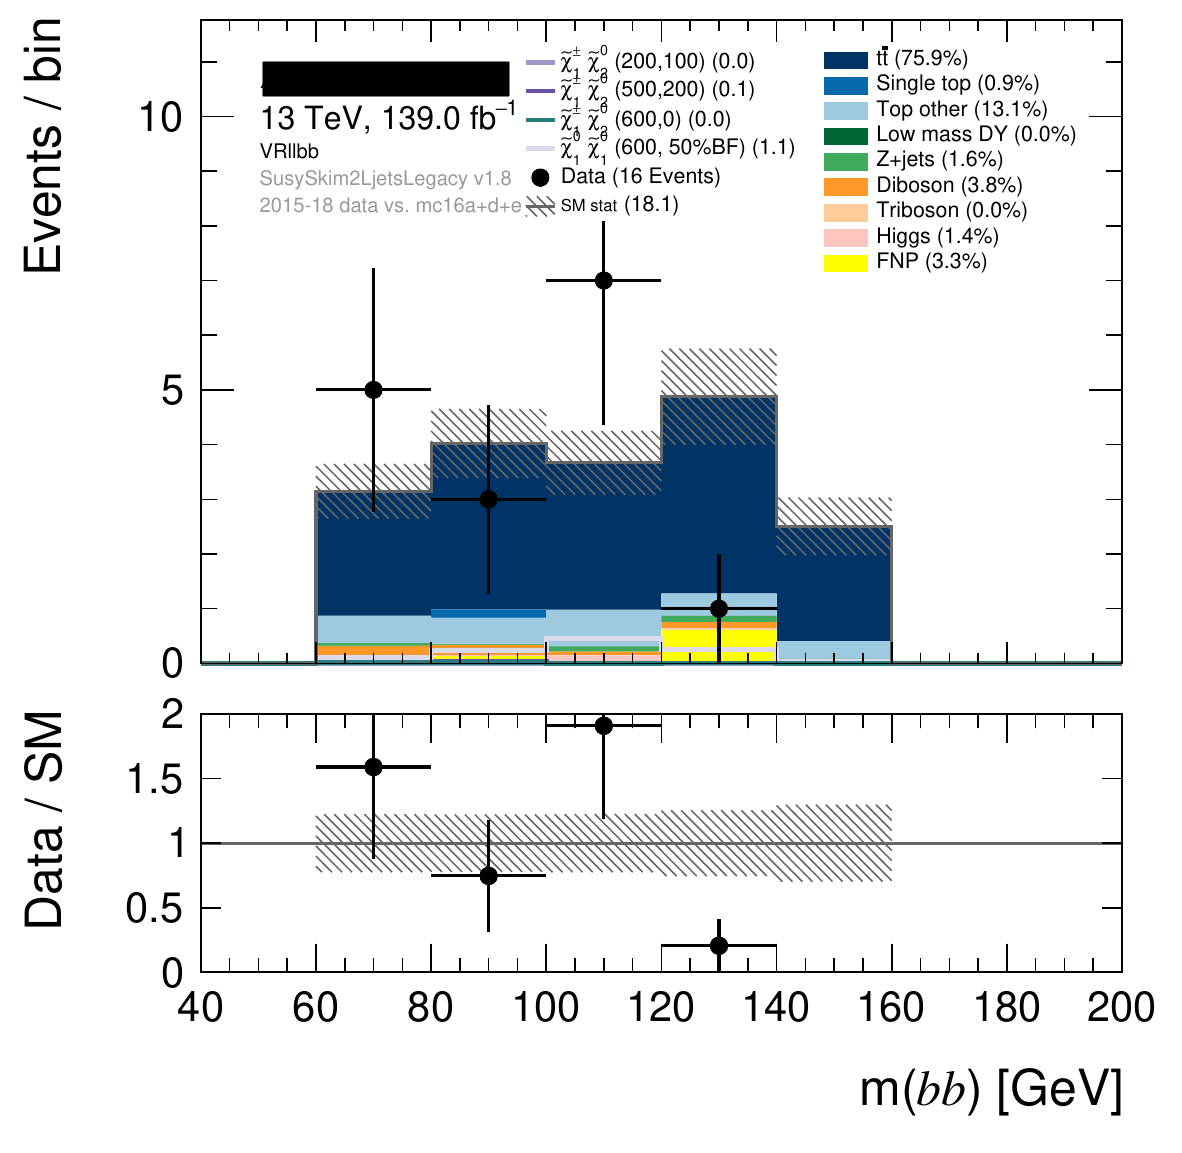
\includegraphics[width=\textwidth]{figures/2ljets_def_mbb_VRllbb.png}
\caption{VR-$\llbb$, $\mbb$}
\end{subfigure}
\caption[
Pre-fit distributions in $\llbb$ signal and validation regions
]{%
Pre-fit distributions in $\llbb$ signal and validation regions.
Signal regions are unblinded.
Errors are statistical.
}
\label{fig:2ljets_high_llbb_region}
\end{figure}

Validation regions, as always, are defined near to each signal region, under
the constraint of being somehow `nearby' and having enough data to test
background predictions.
For SR-High, inverting the selections on $\mjj$ or $\rjj$ satisfies
these criteria, so one validation region is designed on each.
An apparent excess appears at small $\mjj$ in VR-High, which is shown in
Figure~\ref{fig:2ljets_high_mjj_vrhigh}.

Various validation studies explored similar selections and different
simulated samples, and found no clear explanation for this effect.
It therefore motivates the second validation region VR-High-R, and is one
reason for including a lower bound of $\mjj > 20\,\eV[G]$ in all regions.
As seen in Figures~\ref{fig:2ljets_high_region}
and~\ref{fig:2ljets_high_mjj_vrhigh}, VR-High and VR-High-R otherwise show
acceptable pre-fit modelling even without systematic uncertainties.

\begin{figure}[tp]
\centering
\begin{subfigure}{0.48\textwidth}
\centering
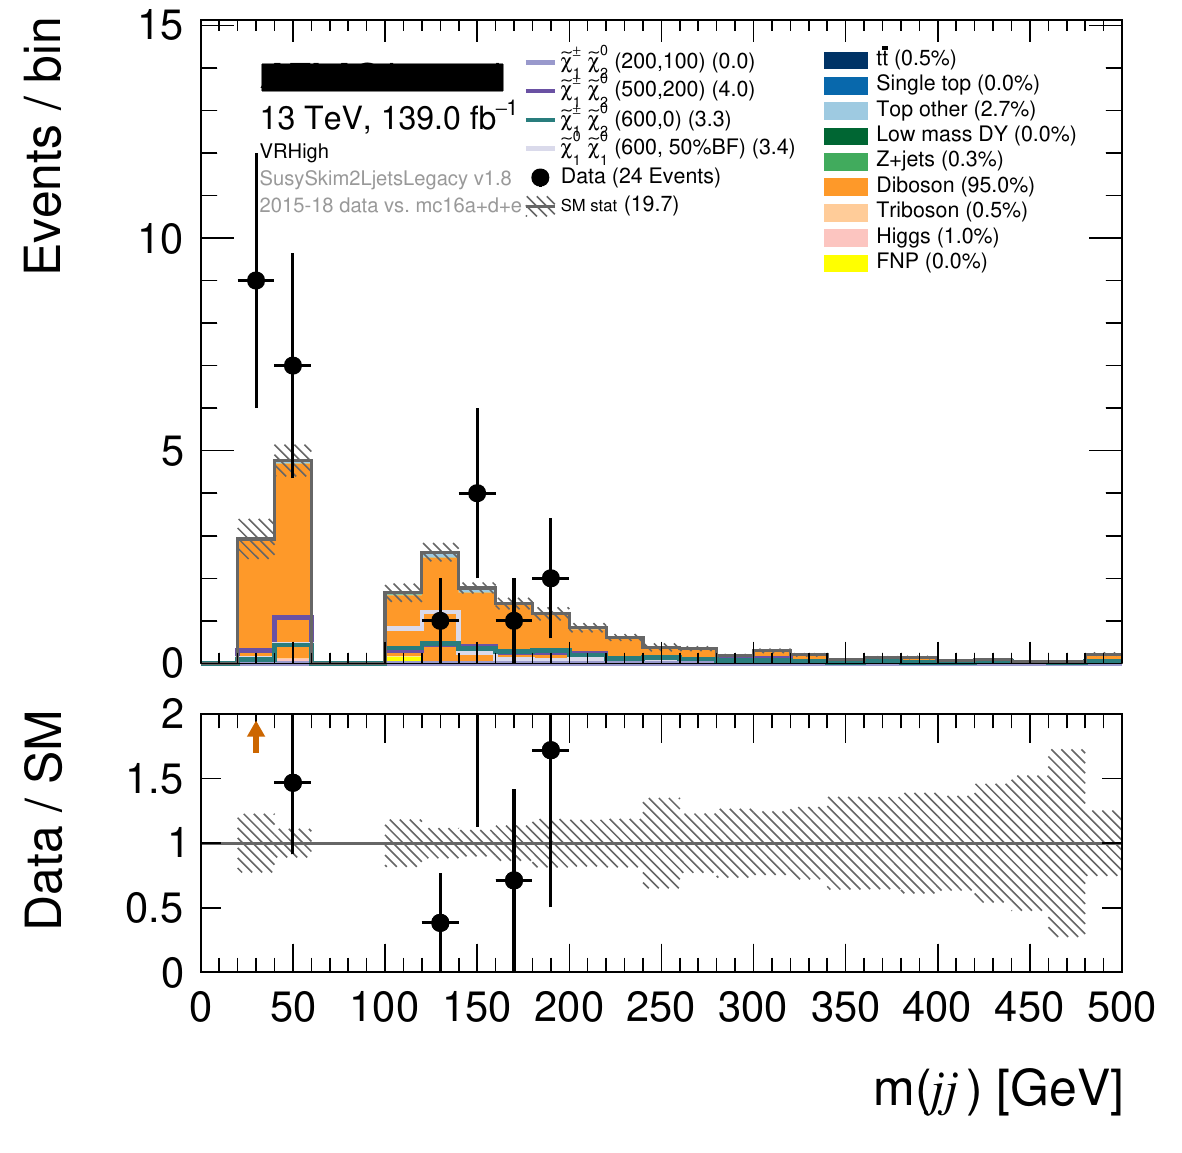
\includegraphics[width=\textwidth]{figures/2ljets_def_mjj_VRHigh.png}
\caption{VR-High, $\mjj$}
\end{subfigure}
\hfill
\begin{subfigure}{0.48\textwidth}
\centering
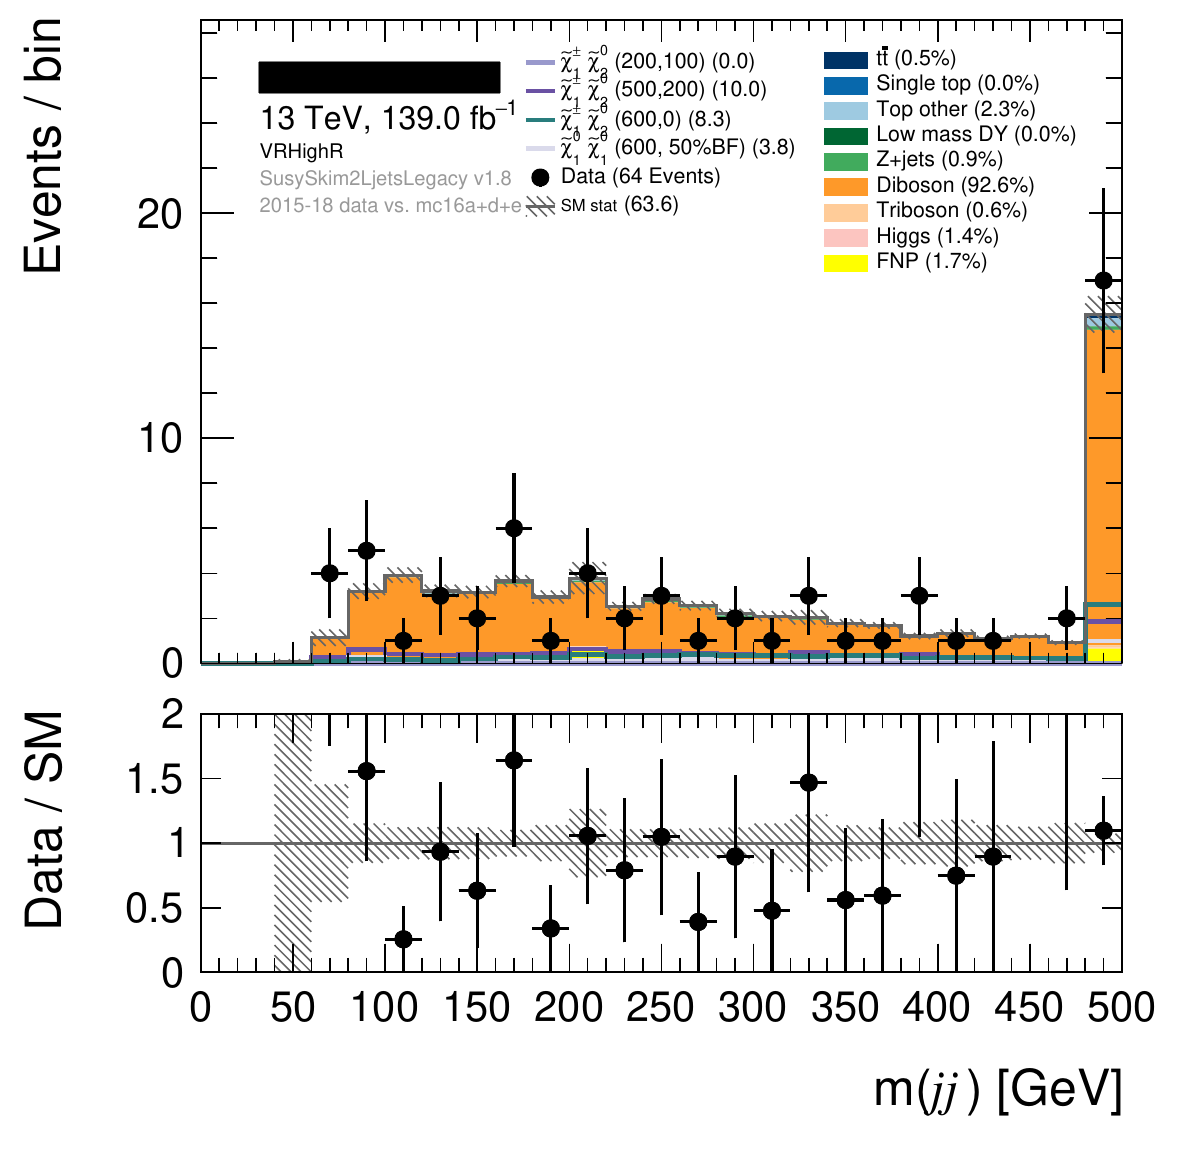
\includegraphics[width=\textwidth]{figures/2ljets_def_mjj_VRHighR.png}
\caption{VR-High-R, $\mjj$}
\end{subfigure}
\caption[
Pre-fit $\mjj$ distributions in validation regions VR-High and VR-High-R
]{%
Pre-fit $\mjj$ distributions in validation regions VR-High and VR-High-R.
Signal regions are unblinded.
Errors are statistical.
The apparent excess at low $\mjj$ in VR-High is not well understood.
}
\label{fig:2ljets_high_mjj_vrhigh}
\end{figure}

The distribution of mono-jet masses $\mjetone$ is sharply peaked towards zero,
so cutting this out while inverting the $\mjetone$ selection of SR-High-1J
more clearly inspects the modelling of massive jets, which appears to be good.
Note that the region $\mjetone > 110$ is also checked in this validation region
and seen to contain no data.
This is good for the standard model.
Since background estimates are near zero up there, non-zero data would have
ruled out our modelling in favour of any model making small positive
predictions.

The small yields beside SR-$\llbb$ in other event variables left $\metsig$ as
the only appropriate candidate to change for VR-$\llbb$.
Unfortunately, this region mostly checks $\ttbar$ backgrounds, and not the
rare $\ttbar Z$ backgrounds which we would most like to validate.
Early work observed good $\ttbar Z$ modelling in three- and four- lepton
selections, but these were excluded from the $\twoljets$ analysis for
orthogonality from other \atlas\ searches with which our results are to be
combined.

Total backgrounds predict data well in VR-$\llbb$.
What was not appreciated soon enough, however, was an excess in the $\metsig$
tail of this region, which is reproduced from the paper in
Figure~\ref{fig:2ljets_high_metsig_vrllbb_paper},
The highest bins have very small background predictions and positive data.
Had this been noticed before unblinding, more validation might have
been advisable.
``In the end'', comments one \atlas\ author,
``it seems fine since there's not events in the SR!''~\cite{comment2022vrllbb}.

\begin{figure}[tp]
\centering
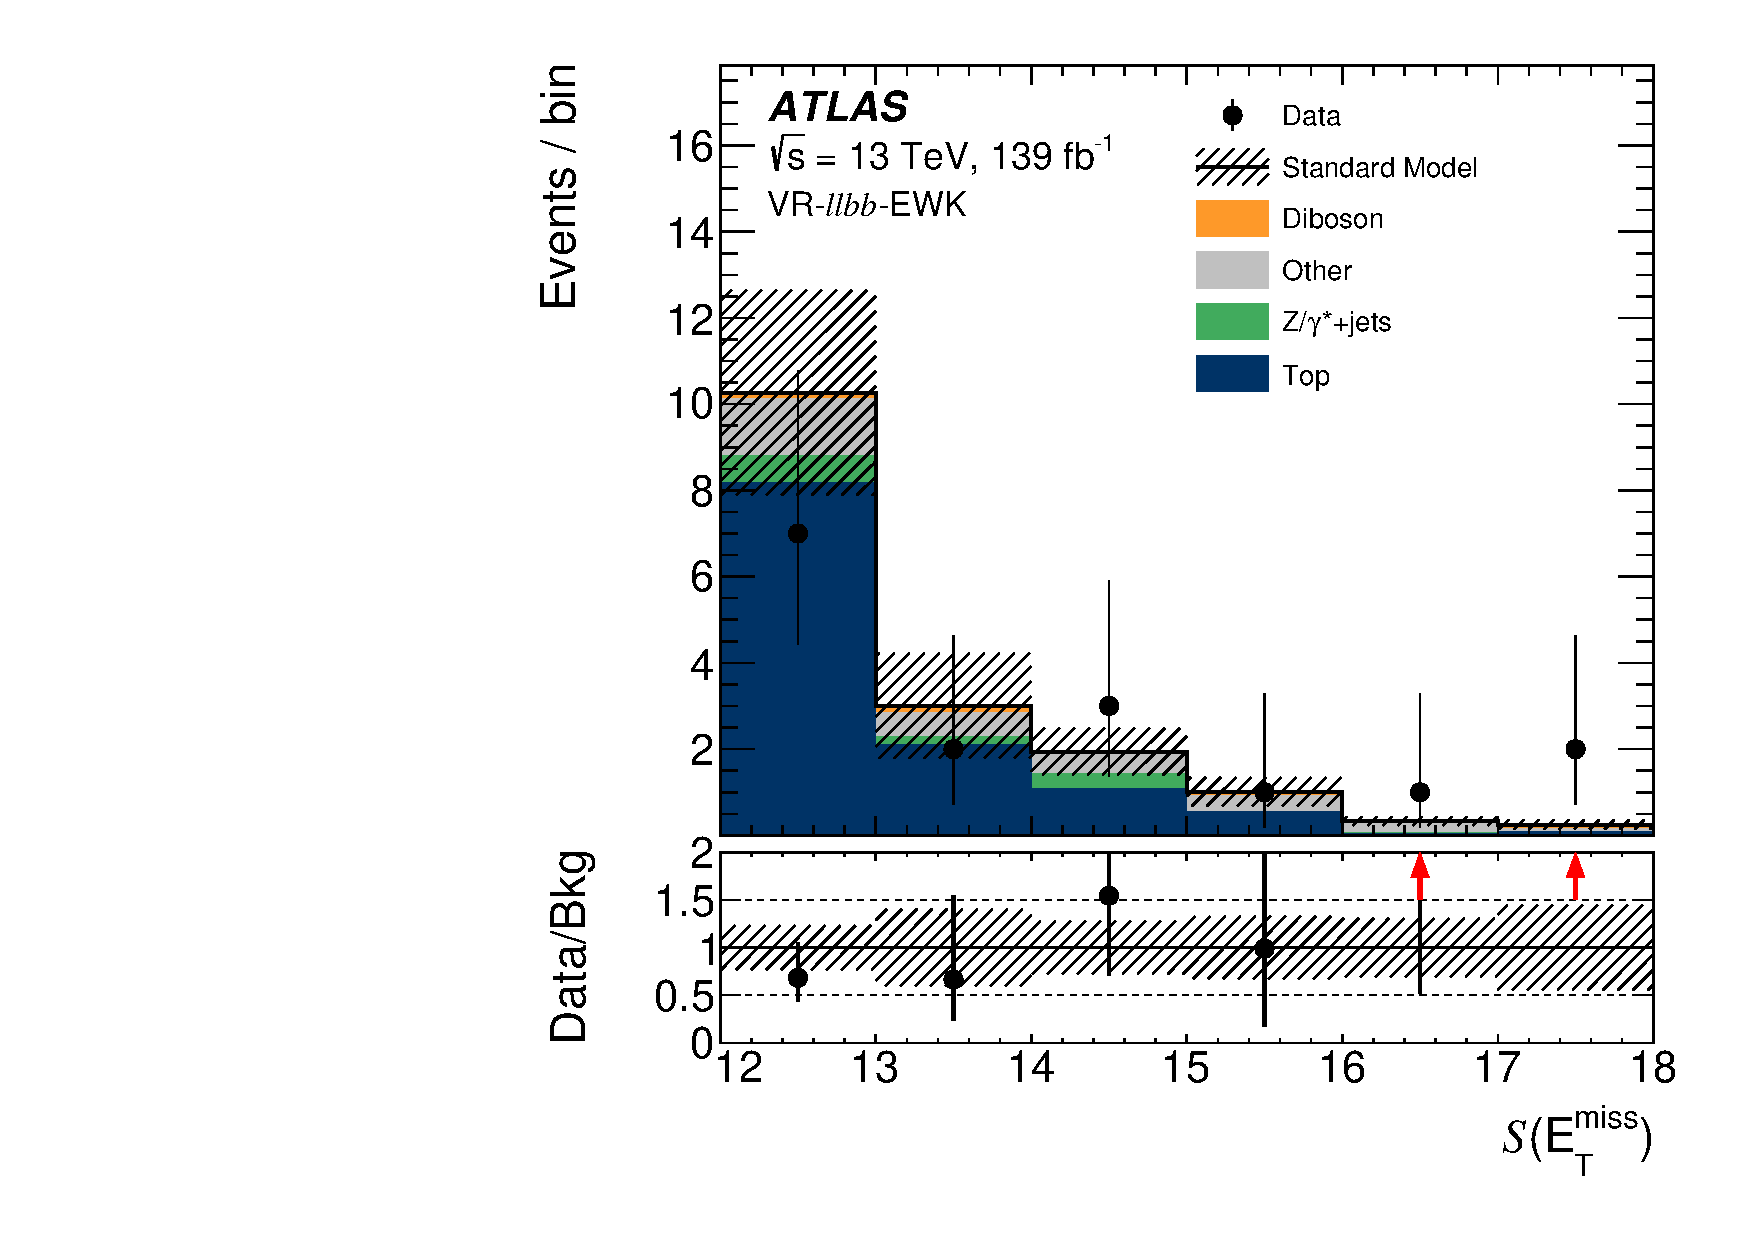
\includegraphics[width=0.48\textwidth]{figures/2ljets_vr_llbb_met_sig.pdf}
\caption[
Post-fit $\metsig$ distribution in VR-$\llbb$
]{%
Post-fit $\metsig$ distribution in VR-$\llbb$.
Backgrounds are to control and signal regions.
This region is also displayed pre-fit with coarser bins in
Figure~\ref{fig:2ljets_high_llbb_region}.
}
\label{fig:2ljets_high_metsig_vrllbb_paper}
\end{figure}


\FloatBarrier
\subsection{Intermediate}
\label{sec:2ljets_int}

Intermediate signal regions are defined to sit in the $\metsig$ range of
$12$ to $18$.
As seen from Figure~\ref{fig:2ljets_presel_met}, this space suffers from
$\ttbar$ background contributions, but it also receives substantial signal
yields from some lighter signal models.
The larger rates of background processes in this space also make it ripe for
control regions.

Intermediate signal regions are defined in Table~\ref{tab:2ljets_int},
along with their associated validation regions and the control regions in this
space.
To suppress the increased backgrounds, the intermediate $\mll$ window is
tightened to reduce non-$Z$ backgrounds, including $\ttbar$ and diboson
processes.
Requiring zero $b$-tags further reduces $\ttbar$ backgrounds.

\begin{table}[tp]
\centering
\begin{tabular}{lccccc}
& $\njet$
& $\nbtag$
& $\metsig$
& $\mjj$
& $\ptjone$
\\[1em]
SR-Int
& $\geq 2$
& $\hphantom{\geq}~0$
& $12\textrm{--}15\textrm{--}18$
& $60\textrm{--}110$
& $> 60$
\\[0.5em]
\: VR-Int
& $\geq 2$
& $\hphantom{\geq}~0$
& $12\textrm{--}18$
& $60\textrm{--}110$
& $\uwave{< 60}$
\\[1em]
CR-VZ
& $\geq 2$
& $\hphantom{\geq}~0$
& $12\textrm{--}18$
& $\uwave{20\textrm{--}60 \mid 110\textrm{--}\infty}$
& $\uwave{\hphantom{< 60}}$
\\[0.5em]
CR-tt
& $\geq 2$
& $\uwave{\geq 1}$
& $\uwave{9\textrm{--}12}$
& $\uwave{20}$
& $> 60$
\end{tabular}
\\[1em]
Common: Pre-selection,
$\njet \geq 2$,
$\mll \in 81\textrm{--}101$, and
$\mttwoll > 80$.
\caption[
Intermediate region definitions in the $\twoljets$-electroweak analysis
]{%
Intermediate region definitions in the $\twoljets$-electroweak analysis.
En-dashes `$a\textrm{--}b$' indicate open intervals $(a, b)$.
Concatenated intervals `$a\textrm{--}b\textrm{--}c$' indicate binning
with boundaries at $a$, $b$, and $c$.
The mid-bar `$\mid$' indicates logical or.
Differences between regions are \uwave{underlined}.
}
\label{tab:2ljets_int}
\end{table}

The less extreme signal models targeted here have less boosted
$W\rightarrow jj$ distributions, and so it was found that a $\ptjone$ selection
was effective at separating signals;
a $\ptjone > 60\,\eV[G]$ requirement split SR-Int from its validation region,
VR-Int and is seen from Figure~\ref{fig:2ljets_int_region} to retain most
signal contributions.
Following our standard pattern set with other signal regions, SR-Int is binned
in $\metsig$ in intervals of $3$ units to improve signal sensitivity.

\begin{figure}[tp]
\centering
\begin{subfigure}{0.48\textwidth}
\centering
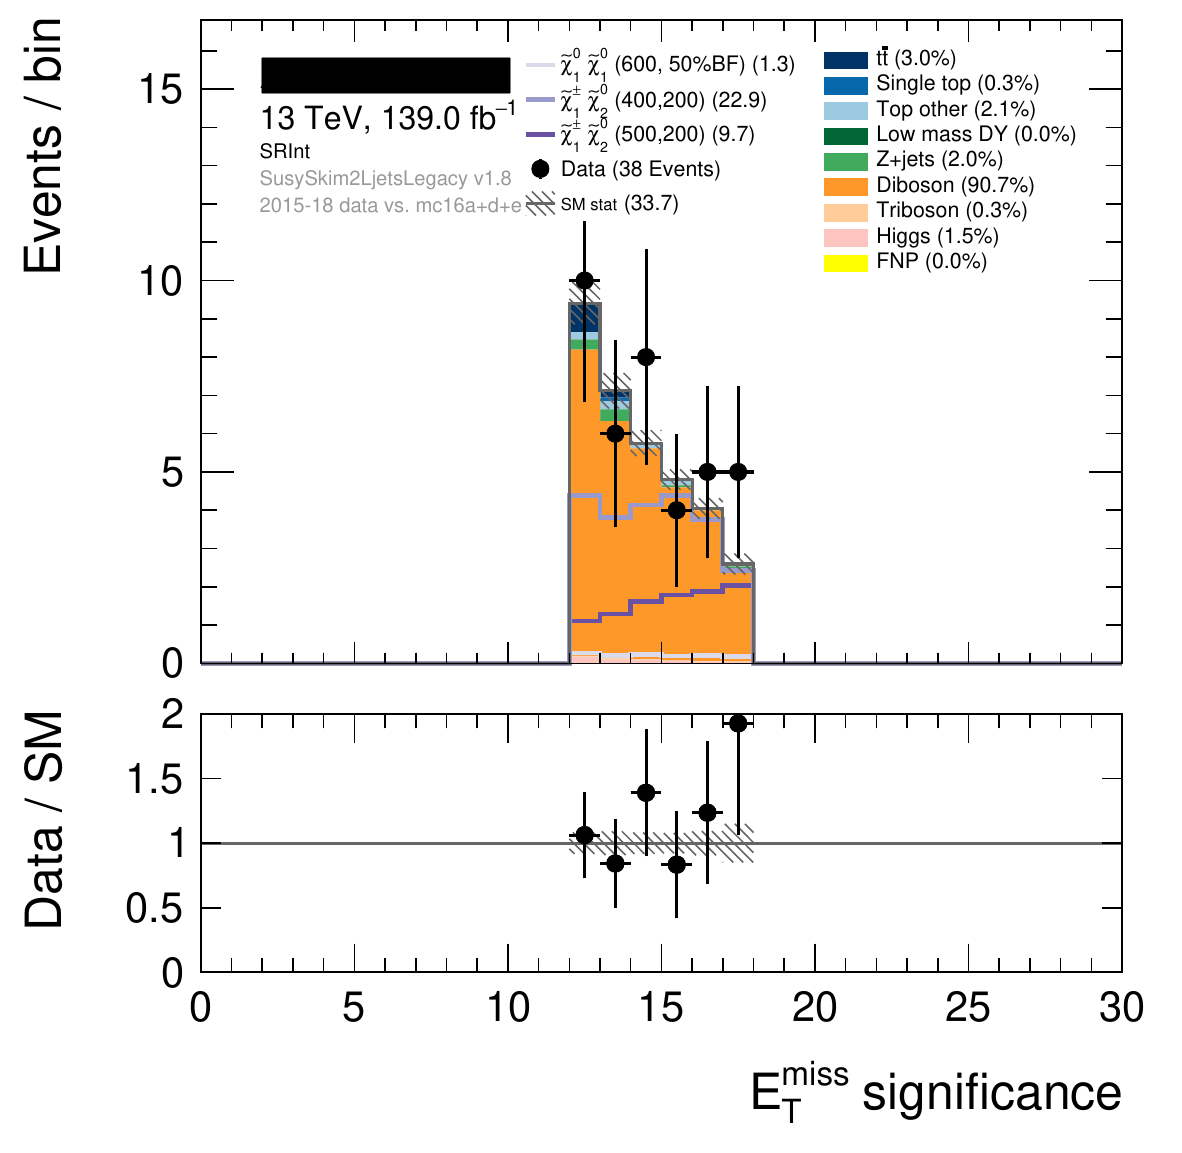
\includegraphics[width=\textwidth]{figures/2ljets_def_met_Sign_SRInt.png}
\caption{SR-Int, $\metsig$}
\end{subfigure}
\hfill
\begin{subfigure}{0.48\textwidth}
\centering
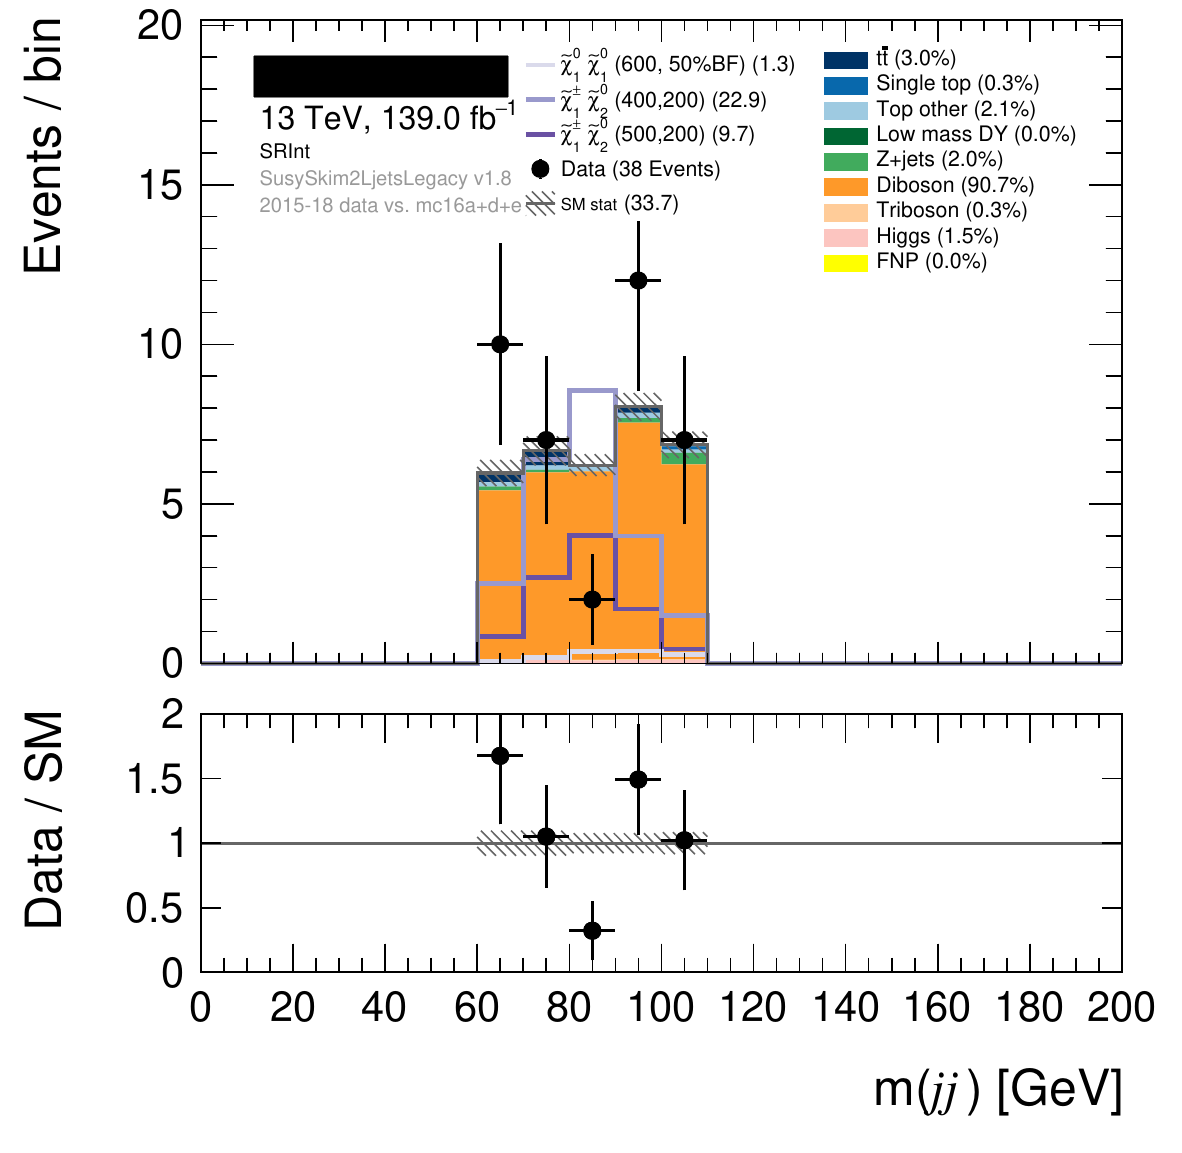
\includegraphics[width=\textwidth]{figures/2ljets_def_mjj_SRInt.png}
\caption{SR-Int, $\mjj$}
\end{subfigure}
\\[0.5em]
\begin{subfigure}{0.48\textwidth}
\centering
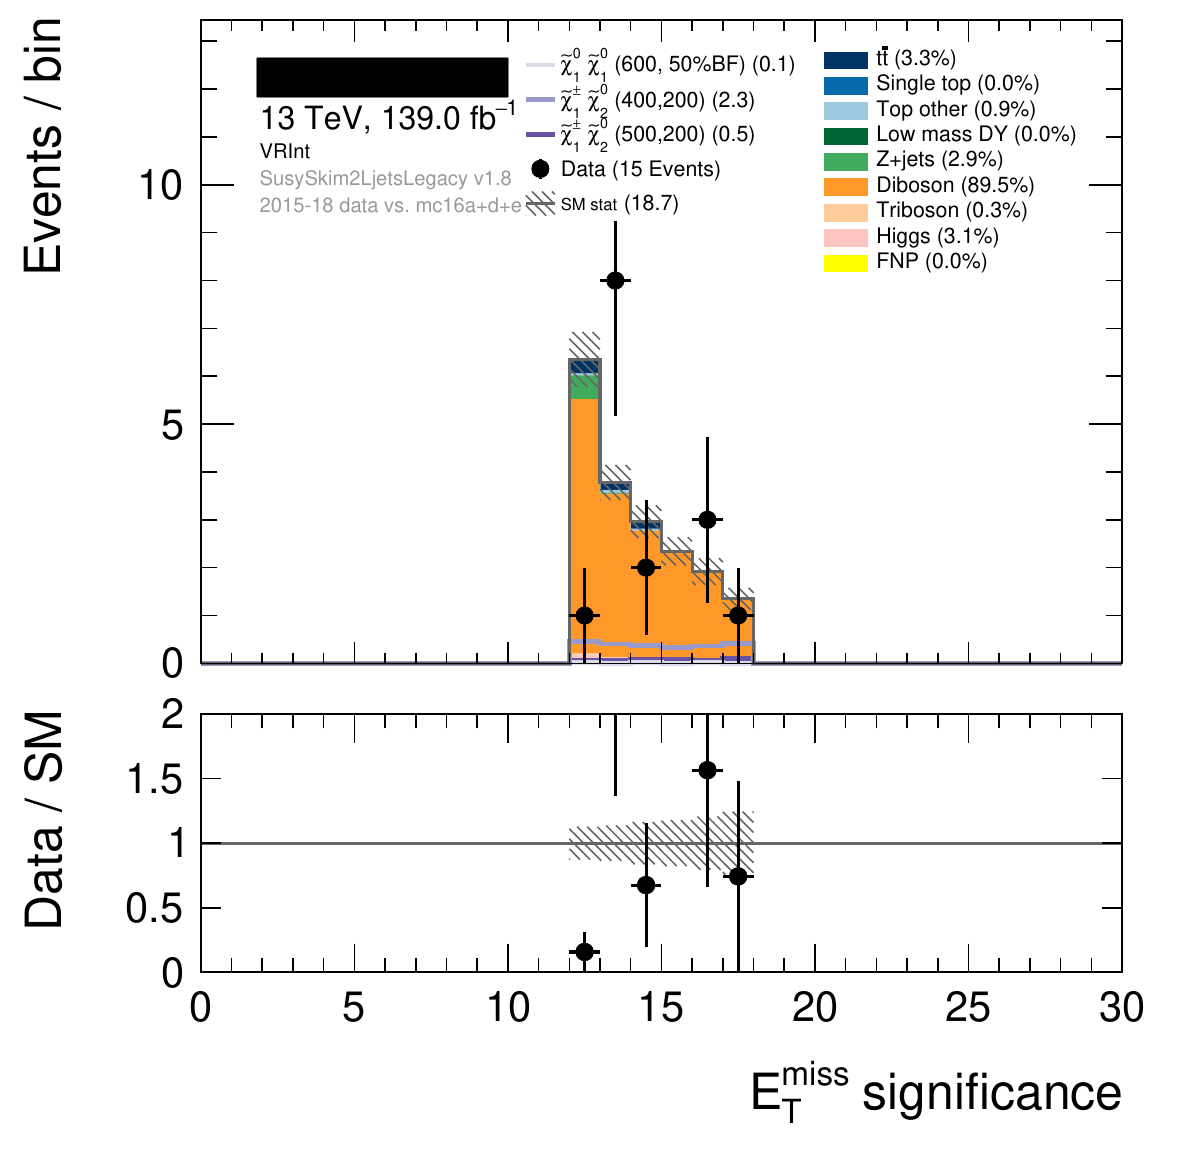
\includegraphics[width=\textwidth]{figures/2ljets_def_met_Sign_VRInt.png}
\caption{VR-Int, $\metsig$}
\end{subfigure}
\hfill
\begin{subfigure}{0.48\textwidth}
\centering
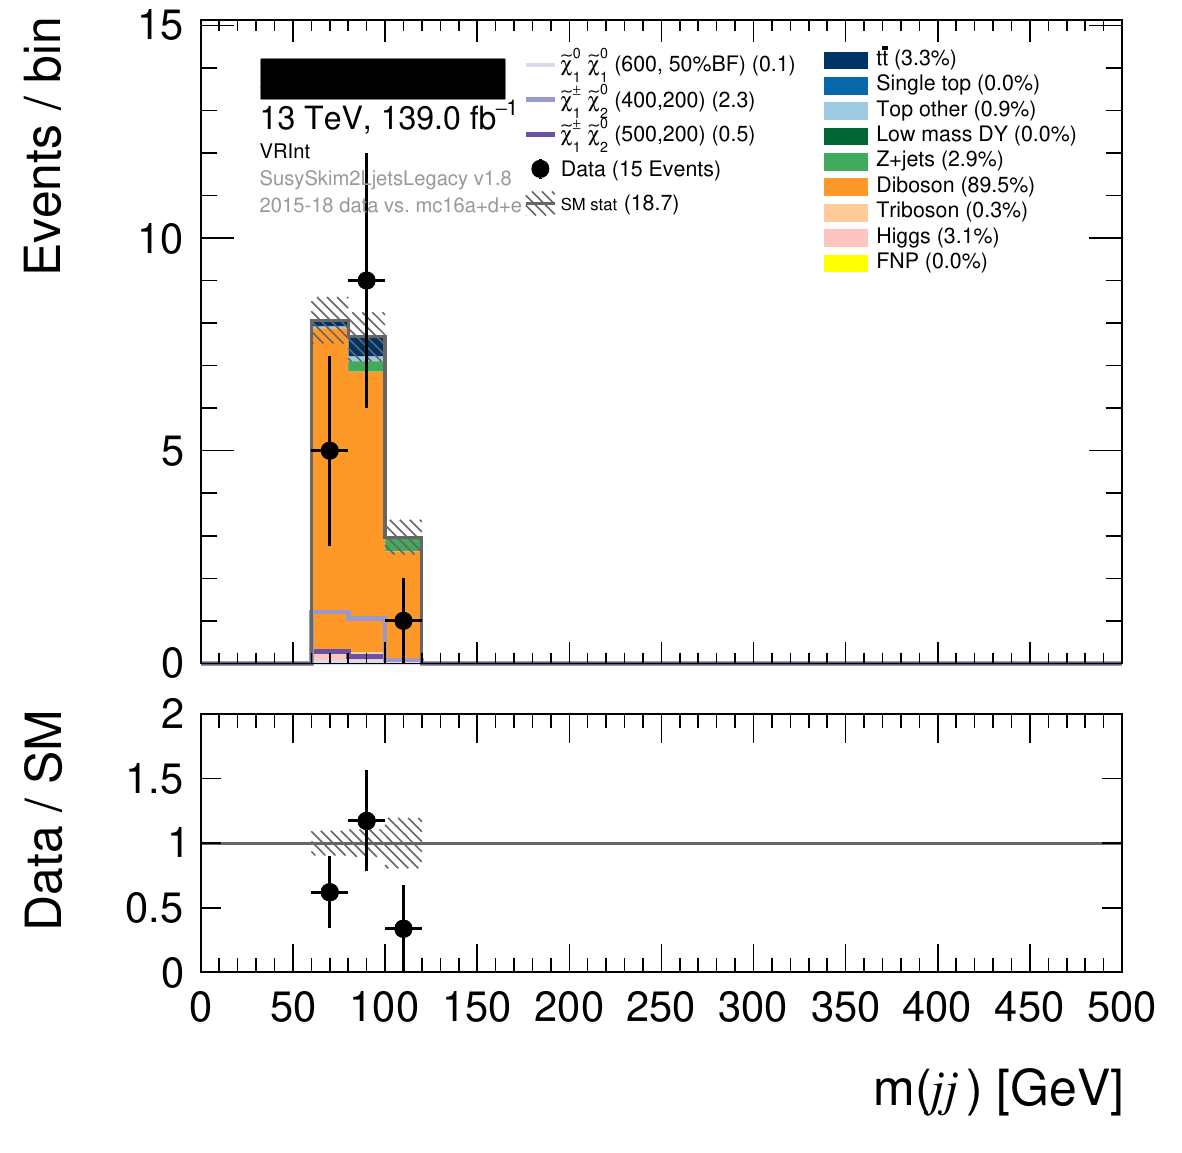
\includegraphics[width=\textwidth]{figures/2ljets_def_mjj_VRInt.png}
\caption{VR-Int, $\mjj$}
\end{subfigure}
\caption[
Pre-fit distributions in Intermediate signal and validation regions
]{%
Pre-fit distributions in Intermediate signal and validation regions.
Signal regions are unblinded.
Errors are statistical.
}
\label{fig:2ljets_int_region}
\end{figure}

The control region CR-VZ is defined on the $\mjj$ side-band to
SR-Int and VR-Int.
As seen from Figure~\ref{fig:2ljets_int_cr_region}, the selections in this
intermediate space give CR-VZ a very pure diboson background, which is very
valuable or constraining the modelling of High regions.
Also included in Table~\ref{tab:2ljets_int} and
Figure~\ref{fig:2ljets_int_cr_region} is CR-tt, which uses various other
selections of $b$-tagged data to constrain $\ttbar$ backgrounds.
Both control regions show good agreement pre-fit and with statistical uncertainties
only.
\begin{figure}[tp]
\centering
\begin{subfigure}{0.48\textwidth}
\centering
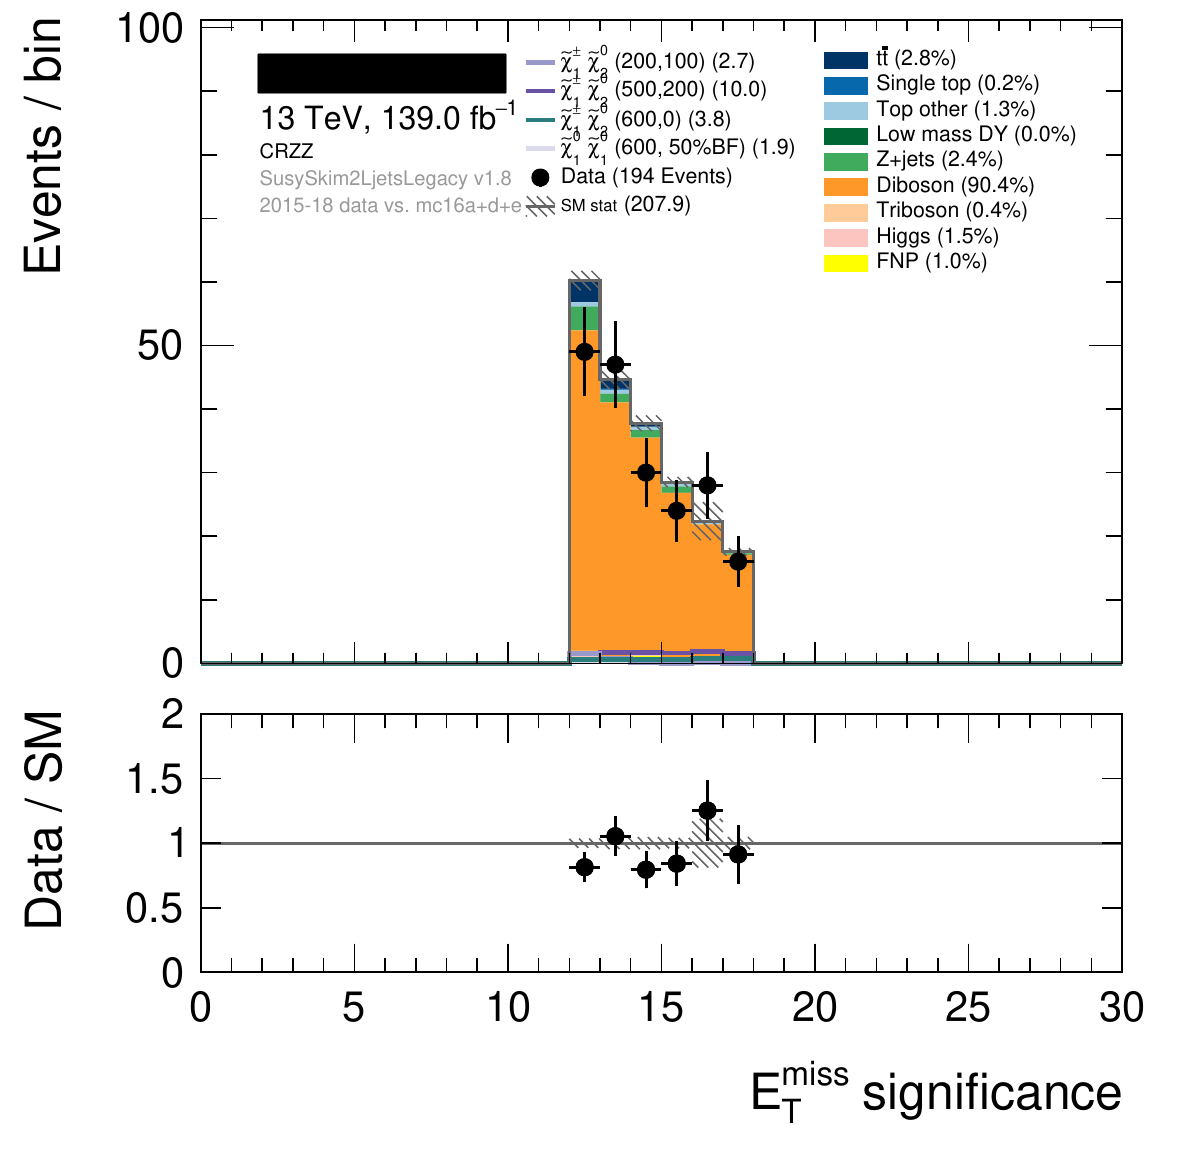
\includegraphics[width=\textwidth]{figures/2ljets_def_met_Sign_CRZZ.png}
\caption{CR-VZ, $\metsig$}
\end{subfigure}
\hfill
\begin{subfigure}{0.48\textwidth}
\centering
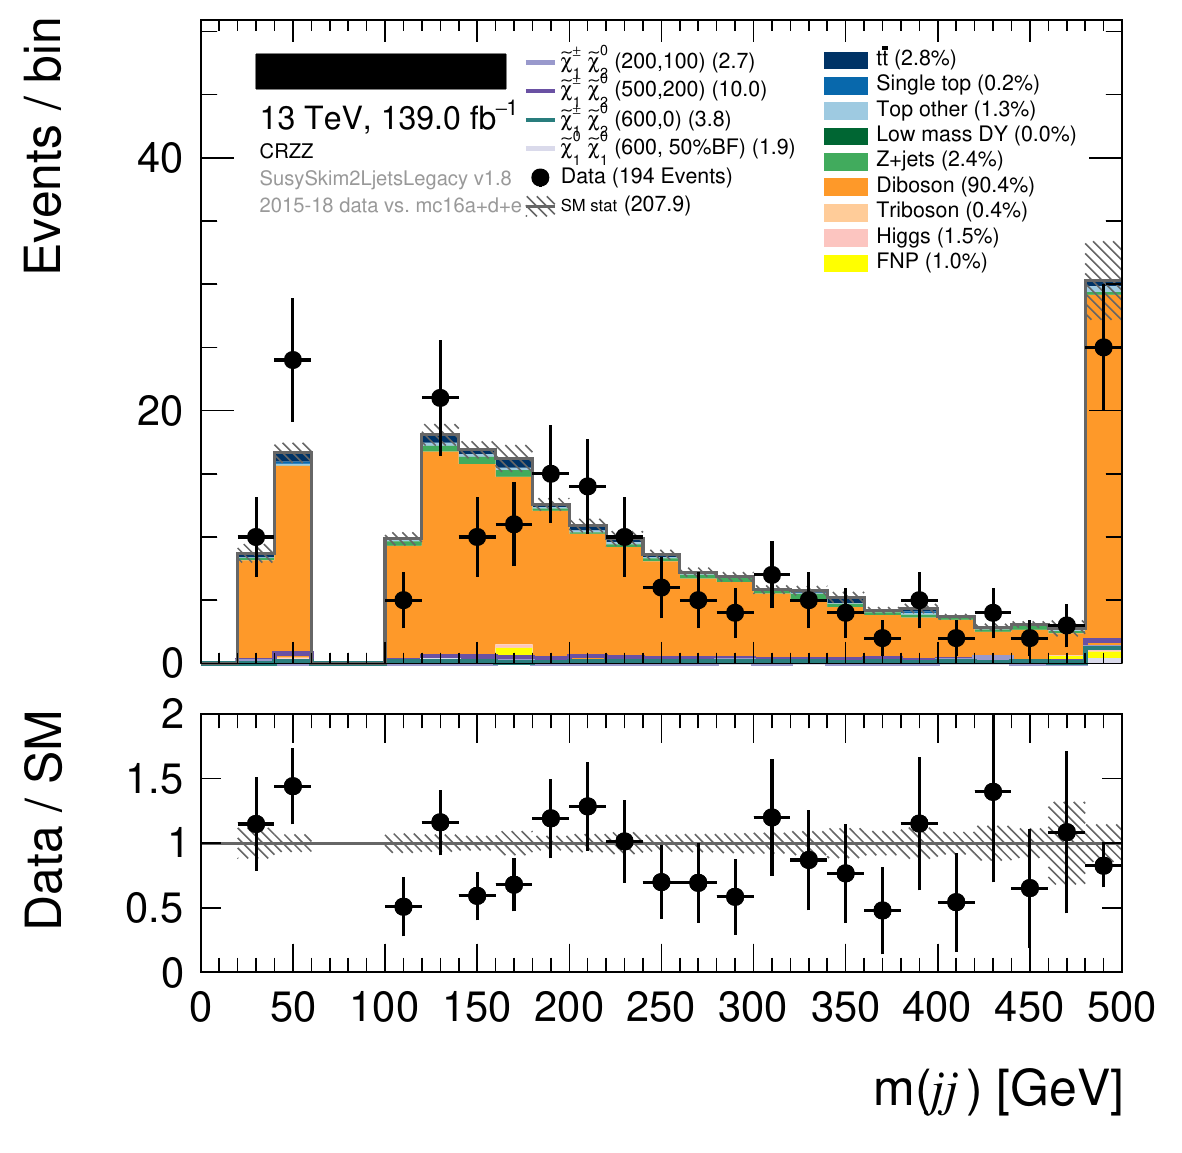
\includegraphics[width=\textwidth]{figures/2ljets_def_mjj_CRZZ.png}
\caption{CR-VZ, $\mjj$}
\end{subfigure}
\\[0.5em]
\begin{subfigure}{0.48\textwidth}
\centering
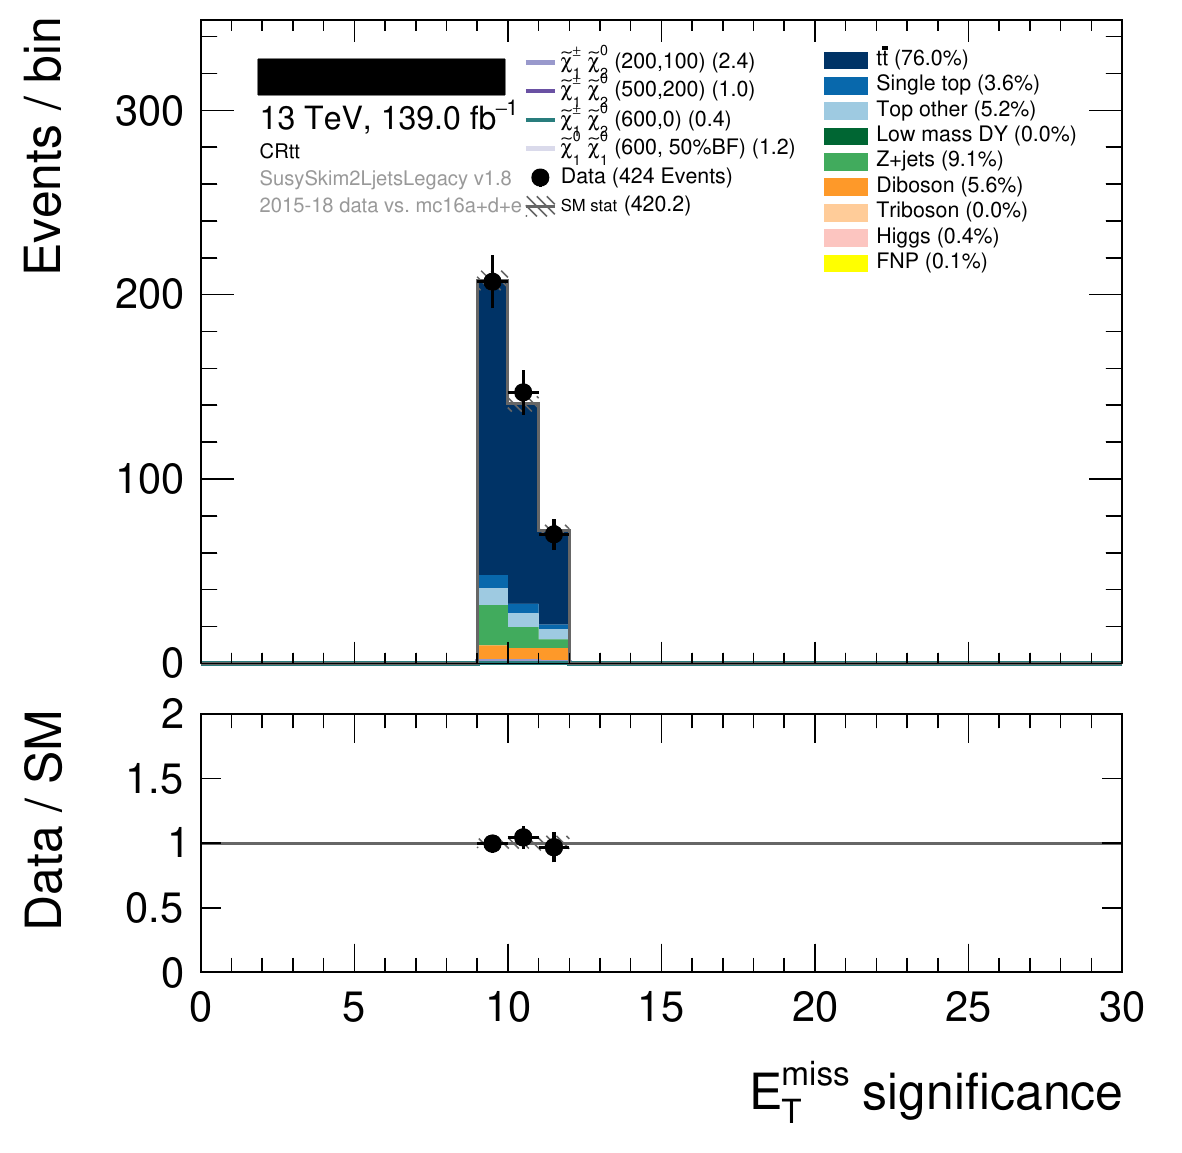
\includegraphics[width=\textwidth]{figures/2ljets_def_met_Sign_CRtt.png}
\caption{CR-tt, $\metsig$}
\end{subfigure}
\hfill
\begin{subfigure}{0.48\textwidth}
\centering
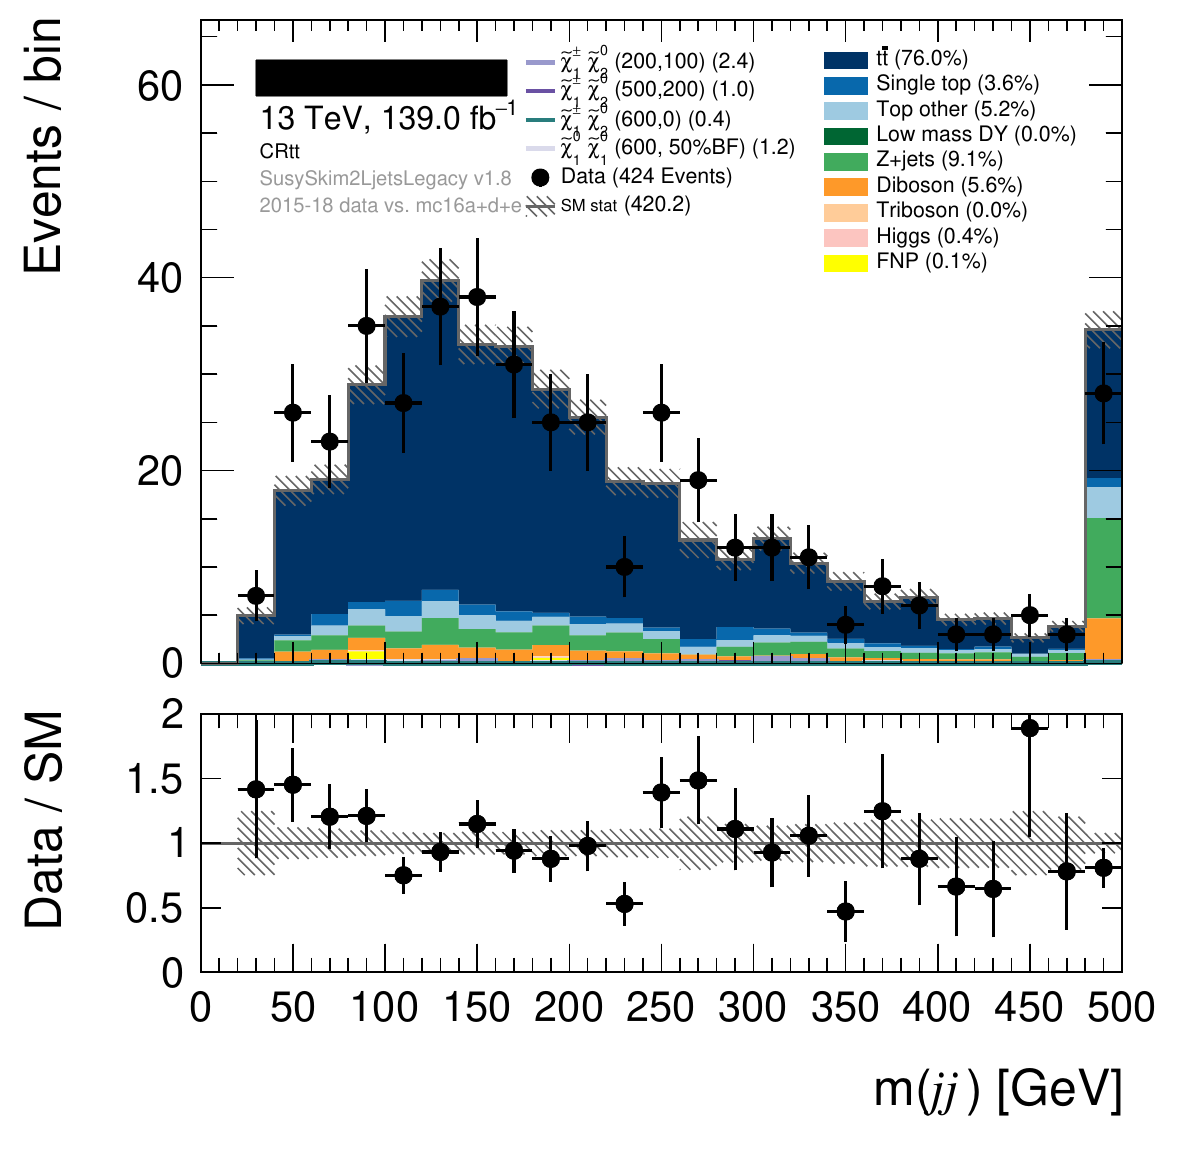
\includegraphics[width=\textwidth]{figures/2ljets_def_mjj_CRtt.png}
\caption{CR-tt, $\mjj$}
\end{subfigure}
\caption[
Pre-fit distributions in the control regions CR-tt and CR-VZ
]{%
Pre-fit distributions in the control regions CR-tt and CR-VZ.
Errors are statistical.
}
\label{fig:2ljets_int_cr_region}
\end{figure}

Some figures label CR-VZ as `CR-ZZ'; the region was renamed late in this
analysis project when it was show to contain substantial fractions of $WZ$
as well as $ZZ$, as illustrated in Figure~\ref{fig:2ljets_splits} of
Section~\ref{sec:2ljets_validation}.


\FloatBarrier
\subsection{Low}
\label{sec:2ljets_low}

In Low regions, which have $\metsig \in 6\textrm{--}12$, the $\zjets$
background becomes a large since its fake $\met$, which arises from
from mismeasurements or rare interactions, is no longer eliminated.
Similarly, backgrounds from $\ttbar$ increase; the selections inherited from
Intermediate regions to suppress $\ttbar$ need supplementing.

Angular selections on lepton variables $\rll$ and $\dphillmet$ characterize
the Low regions, which are defined in Table~\ref{tab:2ljets_low}.
These angular variables usefully reject backgrounds including $\ttbar$, and
provide signal sensitivity to benchmark signal models, as illustrated in
Figure~\ref{fig:2ljets_low_minus};
signals with small mass-splittings of around $100\textrm{--}150\,\eV[G]$
are targetted.

To remove some observed mis-modelling of backgrounds, Low regions require
exactly two jets.
Abandoned region designs which used more jets are discussed below in
Section~\ref{sec:2ljets_low_isr}.

\begin{table}[tp]
\centering
\begin{tabular}{lcccccccc}
& $\metsig$
& $\mjj$
& $\mttwoll$
& $\rll$
& $\dphillmet$
\\[1em]
SR-Low
& $6\textrm{--}9\textrm{--}12$
& $60\textrm{--}110$
& $> 80$
& $< 1$
&
\\[0.5em]
\: VR-Low
& $6\textrm{--}12$
& $60\textrm{--}110$
& $>80$
& $\uwave{1\textrm{--}1.4}$
&
\\[1em]
SR-Low-2
& $6\textrm{--}9$
& $60\textrm{--}110$
& $< 80$
& $< 1.6$
& $< 0.6$
\\[0.5em]
\: VR-Low-2
& $6\textrm{--}9$
& $\uwave{20\textrm{--}60 \mid 110\textrm{--}\infty}$
& $< 80$
& $< 1.6$
& $< 0.6$
\\[1em]
CR-Z
& $6\textrm{--}9$
& $\uwave{20\textrm{--}60 \mid 110\textrm{--}\infty}$
& $> 80$
& $\uwave{\hphantom{< 1.6}}$
& $\uwave{\hphantom{< 0.6}}$
\end{tabular}
\\[1em]
Common: Pre-selection,
$\njet = 2$,
$\nbtag = 0$, and
$\mll \in 81\textrm{--}101$.
\caption[
Low region definitions in the $\twoljets$-electroweak analysis
]{%
Low region definitions in the $\twoljets$-electroweak analysis.
En-dashes `$a\textrm{--}b$' indicate open intervals $(a, b)$.
Concatenated intervals `$a\textrm{--}b\textrm{--}c$' indicate binning
with boundaries at $a$, $b$, and $c$.
The mid-bar `$\mid$' indicates logical or.
Differences between regions are \uwave{underlined}.
}
\label{tab:2ljets_low}
\end{table}

Boosted $Z\rightarrow \ell^+\ell^-$ decays will tend to have small $\rll$.
Similarly to $\rjj$ in the High regions, this can usefully select signals,
but here also works to reject other $\ell^+\ell^-$ production mechanisms which
produce leptons is less correlated directions, particularly dileptonic
$\ttbar$.
As elsewhere, binning of SR-Low in $\metsig \in 6\textrm{--}9\textrm{--}12$
to form SR-Low-a and SR-Low-b respectively, increases sensitivity.

Unblinded, pre-fit histograms of SR-Low are shown in
Figure~\ref{fig:2ljets_low_region}.
Note that these plots do not include systematic uncertainties, so the meaning
of the observed data deficits cannot yet be fully interpreted.
This figure also includes VR-Low, which observes the high $\rll$ edge and
predicts the data well.

\begin{figure}[tp]
\centering
\begin{subfigure}{0.48\textwidth}
\centering
\includegraphics[width=\textwidth]{figures/2ljets_low_Rll_SRLow_noRll.pdf}
\caption{SR-Low$/\{\rll\}$}
\end{subfigure}
\hfill
\begin{subfigure}{0.48\textwidth}
\centering
\includegraphics[width=\textwidth]{figures/2ljets_low_mt2leplsp_0_SRLow_noRll_nomt2.pdf}
\caption{SR-Low$/\{\rll,\mttwoll\}$}
\label{fig:2ljets_low_minus_norll_nomt2_mt2}
\end{subfigure}
\\[0.5em]
\begin{subfigure}{0.48\textwidth}
\centering
\includegraphics[width=\textwidth]{figures/2ljets_low_absdPhiPllMet_SRLow2_noDphi.pdf}
\caption{SR-Low-2$/\{\dphillmet\}$}
\label{fig:2ljets_low_minus_dphi}
\end{subfigure}
\hfill
\begin{subfigure}{0.48\textwidth}
\centering
\includegraphics[width=\textwidth]{figures/2ljets_low_absdPhiPllMet_SRLow2_noDphi_mg5.pdf}
\caption{SR-Low-2$/\{\dphillmet\}$, alternative}
\label{fig:2ljets_low_minus_dphi_alt}
\end{subfigure}
\caption[
Relaxed versions of SR-Low and SR-Low-2 to motivate their angular selections
]{%
Relaxed versions of SR-Low and SR-Low-2 to motivate their angular selections.
Each removes requirements listed in Table~\ref{tab:2ljets_low}:
(a) SR-Low removes $\rll$,
(b) SR-Low removes $\rll$ and $\mttwoll$,
and
(c, d) SR-Low-2 removes $\dphillmet$.
\\[0.5em]
Signals trend towards small $\rll$, plausibly due to their more boosted
$Z\rightarrow \ell^+\ell^-$ decays; small $\rll$ also suppresses $\ttbar$.
The mass of signals seen at small $\mttwoll$ in (b) motivates the design of
SR-Low-2.
Signals in SR-Low-2 spike at small $\dphillmet$ in (c); better statistical
precision is provided by an alternative $\zjets$ sample in (d).
}
\label{fig:2ljets_low_minus}
\end{figure}

\begin{figure}[tp]
\centering
\begin{subfigure}{0.48\textwidth}
\centering
\includegraphics[width=\textwidth]{figures/2ljets_def_met_Sign_SRLow.png}
\caption{SR-Low, $\metsig$}
\end{subfigure}
\hfill
\begin{subfigure}{0.48\textwidth}
\centering
\includegraphics[width=\textwidth]{figures/2ljets_def_mjj_SRLow.png}
\caption{SR-Low, $\mjj$}
\end{subfigure}
\\[0.5em]
\begin{subfigure}{0.48\textwidth}
\centering
\includegraphics[width=\textwidth]{figures/2ljets_def_met_Sign_VRLow.png}
\caption{VR-Low, $\metsig$}
\end{subfigure}
\hfill
\begin{subfigure}{0.48\textwidth}
\centering
\includegraphics[width=\textwidth]{figures/2ljets_def_mjj_VRLow.png}
\caption{VR-Low, $\mjj$}
\end{subfigure}
\caption[
Pre-fit distributions in Low signal and validation regions
]{%
Pre-fit distributions in Low signal and validation regions.
Signal regions are unblinded.
Errors are statistical.
}
\label{fig:2ljets_low_region}
\end{figure}

Uniquely to Low regions, and signal models with small mass-splitting, it is
seen (in Figure~\ref{fig:2ljets_low_minus_norll_nomt2_mt2}) that substantial
signal yields exist at small $\mttwoll$.
To capture these signals, SR-Low-2 is defined as the only
$\twoljets$-electroweak region with $\mttwoll < 80\,\eV[G]$.
That threshold of $80\,\eV[G]$ is not very important.
After the other selections for SR-Low-2, almost all signal and background
samples are in the spike near $0$;
a lower requirement would make little difference, and $80\,\eV[G]$ matches
other, usually inverted, selections.

As shown in Figure~\ref{fig:2ljets_low_minus_dphi}, signal models peak at small
$\dphillmet$, and backgrounds do not; this motivates the $\dphillmet < 0.6$
requirement, and can be understood since a boosted resonance decaying to
$Z+\mathrm{invisible}$ will tend to send the $Z\rightarrow \ell^+\ell^-$ and
$\ptmiss$ in the same direction.

The distribution $\zjets$ here may be surprising, since its $\ptmiss$ is
usually expected to align with a mismeasured jet.
This is explained by the context of a prior $\mttwoll < 80\,\eV[G]$
requirement:
if $\ptmiss$ is facing away from both leptons, then they have large transverse
masses.
Following its definition as a $\min-\max$ of transverse masses,
given in Section~\ref{sec:2ljets_mt2},
the $\mttwoll$ requirement therefore rejects those events, leaving only the
rarer cases of $\zjets$ with small $\dphillmet$.

Excluding $\metsig \in 9\textrm{--}12$ in SR-Low-2 is also not crucial.
This space contains about $2.3$ background expectation (mostly diboson) and
$\approx 1$ from some benchmark signals, so its inclusion as a single combined
bin not have increased sensitivity.
Its inclusion as an orthogonal bin with small yields would have added excessive
complication, however.

Histograms of SR-Low-2 are shown in Figure~\ref{fig:2ljets_low2_region}.
To get sufficiently large backgrounds, the validation region VR-Low-2 uses
the $\mjj$ side-band, and sees good agreement.

\begin{figure}[tp]
\centering
\begin{subfigure}{0.48\textwidth}
\centering
\includegraphics[width=\textwidth]{figures/2ljets_def_met_Sign_SRLow2.png}
\caption{SR-Low-2, $\metsig$}
\end{subfigure}
\hfill
\begin{subfigure}{0.48\textwidth}
\centering
\includegraphics[width=\textwidth]{figures/2ljets_def_mjj_SRLow2.png}
\caption{SR-Low-2, $\mjj$}
\end{subfigure}
\\[0.5em]
\begin{subfigure}{0.48\textwidth}
\centering
\includegraphics[width=\textwidth]{figures/2ljets_def_met_Sign_VRLow2.png}
\caption{VR-Low-2, $\metsig$}
\end{subfigure}
\hfill
\begin{subfigure}{0.48\textwidth}
\centering
\includegraphics[width=\textwidth]{figures/2ljets_def_mjj_VRLow2.png}
\caption{VR-Low-2, $\mjj$}
\end{subfigure}
\caption[
Pre-fit distributions in Low-2 signal and validation regions
]{%
Pre-fit distributions in Low-2 signal and validation regions.
Signal regions are unblinded.
Errors are statistical.
}
\label{fig:2ljets_low2_region}
\end{figure}

Sadly, the $\zjets$ background in SR-Low-2 has terrible statistical precision
in the central simulated sample due to large weights.
This was not as bad when the region was first designed, but became exaggerated
after reprocessing with a new lepton definition and updated software.
The region is plotted with an alternative sample in
Figure~\ref{fig:2ljets_low_minus_dphi_alt}, which has better precision.

% CR
The $\zjets$ control region CR-Z is displayed in
Figure~\ref{fig:2ljets_low_cr_region}.
Pre-fit agreement with data is quite good, although the overflow bin has a
notable excess.
Standardizing cuts to remove high-$\mjj$ tails (such as requiring
$\mjj < 500\,\eV[G]$) could have made control and validation regions like CR-Z
kinematically closer to the signal regions they are supposed to target,
and at least in this case, I believe such a cut would have improved the
analysis.

\begin{figure}[tp]
\centering
\begin{subfigure}{0.48\textwidth}
\centering
\includegraphics[width=\textwidth]{figures/2ljets_def_met_Sign_CRZ.png}
\caption{CR-Z, $\metsig$}
\end{subfigure}
\hfill
\begin{subfigure}{0.48\textwidth}
\centering
\includegraphics[width=\textwidth]{figures/2ljets_def_mjj_CRZ.png}
\caption{CR-Z, $\mjj$}
\end{subfigure}
\caption[
Pre-fit distributions in the control region CR-Z
]{%
Pre-fit distributions in the control region CR-Z.
Errors are statistical.
}
\label{fig:2ljets_low_cr_region}
\end{figure}

The gap at in CR-Z at $\mjj \in 60\textrm{--}110\,\eV[G]$ is exactly SR-Low.
Their union therefore has a continuous $\mjj$ distribution, which is displayed
in Figure~\ref{fig:2ljets_low_sr_or_cr_region}.
Looking at the signal region alone can give an impression that $\zjets$ is
overestimated.
This plot contradicts that; most of the $\zjets$ distribution is fine;
the strange effect happens where diboson becomes large near $m(W)$.

\begin{figure}[tp]
\centering
\includegraphics[width=0.8\textwidth]{figures/2ljets_low_mjj_SRLow_or_CRZ.pdf}
\caption[
The union of CR-Z and SR-Low
]{%
The union of CR-Z and SR-Low, which exactly fills its gap at
$\mjj \in 60\textrm{--}110\,\eV[G]$.
Data have a substantial dip in exactly that mass window.
Errors are statistical.
}
\label{fig:2ljets_low_sr_or_cr_region}
\end{figure}

\subsubsection{Low-ISR}
\label{sec:2ljets_low_isr}

The Low regions presented in Section~\ref{sec:2ljets_low} resulted from a
hasty redesign shortly before unblinding.

Before that redesign, an multi-jet signal region SR-Low-ISR was included,
with associated validation and control regions,
which required $\njet \geq 3$ and offered some meagre extra sensitivity.
Here, `ISR' stands for Initial-State Radiation, following the naming
of previous \atlas searches including partial Run-2 2/3-lepton
search which we are updating~\cite{atlas_23l_SUSY_2016_24}.

Although initial-state radiation typically refers to soft emissions in
parton showers~\cite{corcella2000initial, bewick2022initial},
our ISR explicitly includes hard emissions from the perturbative matrix element
simulation;
ISR is selected to give a hard transverse boost to the supersymmetric
particles, making their resulting $\met$, and other kinematics, more distinctive.

As an event variable, we follow \cite{atlas_23l_SUSY_2016_24} to define the
ISR momentum as the vector sum of all jets not assigned to the
$W\rightarrow jj$ decay.
This ISR construction does not select the two hardest for the $W$ candidate,
unlike our other regions, but instead takes the two closest in $\phi$ to the
vector $\vec \pt^{\ell\ell} + \ptmiss$;
the two jets selected in this way are used to define the mass $\mwisr$.

The region SR-Low-ISR required $\ptisr > 300\,\eV[G]$ for a substantial
boost and $\dphiisrmet > 2.6$ to catch invisible particles boosted away from the
ISR, along with standard selections $\mwisr \in 60\textrm{--}110\,\eV[G]$,
$\metsig \in 6\textrm{--}12$, and preselection, as well as $\mjj > 110\,\eV[G]$
for orthogonality from other signal regions.

The main ISR regions are shown in Figure~\ref{fig:2ljets_low_isr_old}; no data
are shown in the signal region, since it was never unblinded.
From the validation and control regions, however, there is a clear deficit
of data below backgrounds by about $30\%$.
Here, VR-Low-ISR differs from SR-Low-ISR by requiring
$\ptisr \in 200\textit{--}300\,\eV[G]$, and CR-Low-ISR differs by requiring
$\ptisr > 200\,\eV[G]$ and
$\mwisr \in 20\textrm{--}60 \mid 110\textrm{--}\infty$.

\begin{figure}[tp]
\centering
\begin{subfigure}{0.48\textwidth}
\centering
\includegraphics[width=\textwidth]{figures/2ljets_vrlow_old_srlowisr.png}
\caption{SR-Low-ISR, $\ptisr$ (blind)}
\label{fig:2ljets_low_isr_old_sr}
\end{subfigure}
\\[0.5em]
\begin{subfigure}{0.48\textwidth}
\centering
\includegraphics[width=\textwidth]{figures/2ljets_vrlow_old_vrlowisr.png}
\caption{VR-Low-ISR, $\mwisr$}
\end{subfigure}
\hfill
\begin{subfigure}{0.48\textwidth}
\centering
\includegraphics[width=\textwidth]{figures/2ljets_vrlow_old_crlowisr.png}
\caption{CR-Low-ISR, $\mwisr$}
\end{subfigure}
\caption[
Pre-fit distributions in draft Low-ISR regions
]{%
Pre-fit distributions in draft Low-ISR regions, which were removed and never
unblinded.
These regions required a third, hard jet directed away from $\ptmiss$.
As seen from (b) and (c), the background modelling is poor and in conflict
with normalization factors in other control regions.
Variables and regions are defined in the text of
Section~\ref{sec:2ljets_low_isr}.
Errors are statistical.
}
\label{fig:2ljets_low_isr_old}
\end{figure}

Additional control regions were designed in an attempt to improve background
normalization local to this region.
These are CR-Low-ISR-Z and CR-Low-ISR-DF, which select $\zjets$ and $\ttbar$
backgrounds and find smaller deficits of $20\%$ and $10\%$ respectively,
as shown in Figure~\ref{fig:2ljets_low_isr_old_more}.
To select $\zjets$, CR-Low-ISR-Z differs from CR-Low-ISR by requiring
$\dphiisrmet \in 1\textrm{--}2.6$ and $\metsig \in 6\textrm{--}9$.
To select $\ttbar$, CR-Low-ISR-DF differs from CR-Low-ISR by requiring
different-flavour leptons and the simpler $\mwisr > 20\,\eV[G]$, since it
has no signal regions to avoid in different-flavour data.
No nearby selection was found to form a pure diboson control region near here.

\begin{figure}[tp]
\centering
\begin{subfigure}{0.48\textwidth}
\centering
\includegraphics[width=\textwidth]{figures/2ljets_vrlow_old_crlowisr_z.png}
\caption{CR-Low-ISR-Z, $\mwisr$}
\end{subfigure}
\hfill
\begin{subfigure}{0.48\textwidth}
\centering
\includegraphics[width=\textwidth]{figures/2ljets_vrlow_old_crlowisr_df.png}
\caption{CR-Low-ISR-DF, $\mwisr$}
\end{subfigure}
\caption[
Pre-fit distributions in extra control regions for the draft Low-ISR
]{%
Pre-fit distributions in extra control regions for the draft Low-ISR.
These regions required a third, hard jet directed away from $\ptmiss$.
Variables and regions are defined in the text of
Section~\ref{sec:2ljets_low_isr}.
Errors are statistical.
}
\label{fig:2ljets_low_isr_old_more}
\end{figure}

A complicated likelihood model was constructed which normalized diboson,
$\zjets$ and $\ttbar$ backgrounds to the combination of CR-Low-ISR,
CR-Low-ISR-Z, CR-Low-ISR-DF.
After this fit, the validation region VR-Low-ISR had a high background
of $56.7 \pm 4.4$ for $47$ data, which is only a $1$-sigma deficit.

This complication is a great deal of cost for what is only a weakly sensitive
signal region, reaching only a projected significance $Z\approx 1$ for the
(pre-fit) signals shown in Figure~\ref{fig:2ljets_low_isr_old_sr}.
On the very sound advice of \atlas authors commenting on the internal
documentation, this ISR construction was entirely removed.

Modelling multi-jet QCD is hard.
This deficit was therefore blamed on multi-jet QCD modelling, and resolved by
retreating to two-jet events.
I find it interesting, however, that the two-jet SR-Low did eventually observe
a comparable deficit when unblinded.


\FloatBarrier
\subsection{Off-shell}
\label{sec:2ljets_offshell}
Table~\ref{tab:2ljets_offshell}
Figure~\ref{fig:2ljets_offshell_region}

\begin{table}[tp]
\centering
\begin{tabular}{lccccc}
& $\metsig$
& $\mll$
& $\mttwoll$
& $\ptjone$
& $\dphijmet$
\\[1em]
SR-OffShell
& $>9$
& $12\textrm{--}40\textrm{--}71$
& $>100$
& $>100$
& $>2$
\\[0.5em]
\: VR-OffShell
& $>9$
&  12--71
& $\uwave{80\textrm{--}100}$
& $> 100$
& $> 2$
\\[1em]
CR-DY
& $\uwave{6\textrm{--}9}$
& $12\textrm{--}71$
& $> 100$
& $\uwave{\hphantom{> 100}}$
& $\uwave{\hphantom{> 2}}$
\end{tabular}
\\[1em]
Common: Pre-selection,
$\njet \geq 2$, and
$\nbtag = 0$.
\caption[
Off-shell region definitions in the $\twoljets$-electroweak analysis
]{%
Off-shell region definitions in the $\twoljets$-electroweak analysis.
En-dashes `$a\textrm{--}b$' indicate open intervals $(a, b)$.
Concatenated intervals `$a\textrm{--}b\textrm{--}c$' indicate binning
with boundaries at $a$, $b$, and $c$.
The mid-bar `$\mid$' indicates logical or.
Differences between regions are \uwave{underlined}.
}
\label{tab:2ljets_offshell}
\end{table}

\begin{figure}[tp]
\centering
\begin{subfigure}{0.48\textwidth}
\centering
\includegraphics[width=\textwidth]{figures/2ljets_def_met_Sign_SROffShell.png}
\caption{SR-OffShell, $\metsig$}
\end{subfigure}
\hfill
\begin{subfigure}{0.48\textwidth}
\centering
\includegraphics[width=\textwidth]{figures/2ljets_def_mll_SROffShell.png}
\caption{SR-OffShell, $\mll$}
\end{subfigure}
\\[0.5em]
\begin{subfigure}{0.48\textwidth}
\centering
\includegraphics[width=\textwidth]{figures/2ljets_def_met_Sign_VROffShell.png}
\caption{VR-OffShell, $\metsig$}
\end{subfigure}
\hfill
\begin{subfigure}{0.48\textwidth}
\centering
\includegraphics[width=\textwidth]{figures/2ljets_def_mll_VROffShell.png}
\caption{VR-OffShell, $\mll$}
\end{subfigure}
\caption[
Pre-fit distributions in OffShell signal and validation regions
]{%
Pre-fit distributions in OffShell signal and validation regions.
Signal regions are unblinded.
Errors are statistical.
}
\label{fig:2ljets_offshell_region}
\end{figure}

\begin{figure}[tp]
\centering
\begin{subfigure}{0.48\textwidth}
\centering
\includegraphics[width=\textwidth]{figures/2ljets_def_met_Sign_CRDY.png}
\caption{CR-DY, $\metsig$}
\end{subfigure}
\hfill
\begin{subfigure}{0.48\textwidth}
\centering
\includegraphics[width=\textwidth]{figures/2ljets_def_mll_CRDY.png}
\caption{CR-DY, $\mll$}
\end{subfigure}
\caption{%
Pre-fit distributions in the control region CR-DY.
Errors are statistical.
}
\label{fig:2ljets_offshell_cr_region}
\end{figure}


\FloatBarrier
\subsection{Discovery}
\label{sec:2ljets_disco}

\begin{itemize}
\item DR-High: SR-High-8
\item DR-$\llbb$: SR-$\llbb$
\item DR-Int: SR-Int
\item DR-Low: SR-Low
\item DR-OffShell: SR-OffShell
\end{itemize}

Figure~\ref{fig:2ljets_disco_trials_high}
Figure~\ref{fig:2ljets_disco_trials_llbb}
Figure~\ref{fig:2ljets_disco_trials_int}
Figure~\ref{fig:2ljets_disco_prefit}

\begin{figure}[tp]
\centering
\begin{subfigure}{0.48\textwidth}
\centering
\includegraphics[width=\textwidth]{figures/2ljets_disco_High_C1N2_WZ_500p0_200p0_2L2J.png}
\caption{}
\end{subfigure}
\hfill
\begin{subfigure}{0.48\textwidth}
\centering
\includegraphics[width=\textwidth]{figures/2ljets_disco_High_C1N2_WZ_600_0_2L2J.png}
\caption{}
\end{subfigure}
\caption[
Evaluation of candidate High discovery regions
]{%
Evaluation of candidate High discovery regions.
The region SR-High-8, labelled `High8\_1+\_2' here, is chosen for its
simplicity and good sensitivity to both benchmark signal models.
Upper plots show background and signal yields.
Lower plots show various measures of projected
sensitivity~\cite{cousins2008evaluation}.
Yields are derived in an early iteration of the analysis and do not exactly
match those in the final result.
}
\label{fig:2ljets_disco_trials_high}
\end{figure}

\begin{figure}[tp]
\centering
\begin{subfigure}{0.48\textwidth}
\centering
\includegraphics[width=\textwidth]{figures/2ljets_disco_llbb_C1N2N1_GGMHinoZh50_600.png}
\caption{}
\end{subfigure}
\hfill
\begin{subfigure}{0.48\textwidth}
\centering
\includegraphics[width=\textwidth]{figures/2ljets_disco_llbb_C1N2N1_GGMHinoZh50_700.png}
\caption{}
\end{subfigure}
\caption[
Evaluation of candidate $\llbb$ discovery regions
]{%
Evaluation of candidate $\llbb$ discovery regions.
The region SR-$\llbb$, labelled `SRllbb' here, is chosen for
sensitivity, simplicity, and to avoid overlapping with DR-High.
Upper plots show background and signal yields.
Lower plots show various measures of projected
sensitivity~\cite{cousins2008evaluation}.
Yields are derived in an early iteration of the analysis and do not exactly
match those in the final result.
}
\label{fig:2ljets_disco_trials_llbb}
\end{figure}

\begin{figure}[tp]
\centering
\begin{subfigure}{0.48\textwidth}
\centering
\includegraphics[width=\textwidth]{figures/2ljets_disco_Int_C1N2_WZ_250p0_100p0_2L2J.png}
\caption{}
\end{subfigure}
\hfill
\begin{subfigure}{0.48\textwidth}
\centering
\includegraphics[width=\textwidth]{figures/2ljets_disco_Int_C1N2_WZ_400p0_200p0_2L2J.png}
\caption{}
\end{subfigure}
\caption[
Evaluation of candidate Intermediate discovery regions
]{%
Evaluation of candidate Intermediate discovery regions.
The region SR-Int, labelled `Int\_1+\_2' here, is chosen for its simplicity
and broad sensitivity.
Upper plots show background and signal yields.
Lower plots show various measures of projected
sensitivity~\cite{cousins2008evaluation}.
Yields are derived in an early iteration of the analysis and do not exactly
match those in the final result.
}
\label{fig:2ljets_disco_trials_int}
\end{figure}

\begin{figure}[tp]
\centering
\begin{subfigure}{0.38\textwidth}
\centering
\includegraphics[width=\textwidth]{figures/2ljets_disco_plot_DRHigh.png}
\caption{DR-High}
\end{subfigure}
\quad\quad
\begin{subfigure}{0.38\textwidth}
\centering
\includegraphics[width=\textwidth]{figures/2ljets_disco_plot_DRllbb.png}
\caption{DR-$\llbb$}
\end{subfigure}
\\[0.5em]
\begin{subfigure}{0.38\textwidth}
\centering
\includegraphics[width=\textwidth]{figures/2ljets_disco_plot_DRInt.png}
\caption{DR-Int}
\end{subfigure}
\quad\quad
\begin{subfigure}{0.38\textwidth}
\centering
\includegraphics[width=\textwidth]{figures/2ljets_disco_plot_DRLow.png}
\caption{DR-Low}
\end{subfigure}
\\[0.5em]
\begin{subfigure}{0.38\textwidth}
\centering
\includegraphics[width=\textwidth]{figures/2ljets_disco_plot_DROffShell.png}
\caption{DR-OffShell}
\end{subfigure}
\caption[
Pre-fit yields in discovery regions
]{%
Pre-fit yields in discovery regions.
Errors are statistical.
}
\label{fig:2ljets_disco_prefit}
\end{figure}


\section{Modelling}
% TODO backgorund samples
% TODO matrix method fakes
% TODO GMSB reweighting
% TODO off-shell plus/minus split
% TODO generator filtering


Table~\ref{tab:2ljets_zjets_alt}

\begin{table}[tp]
\centering
\begin{tabular}{lcc}
& Central
& Relative variations
\\[0.5em]
CR-DY
& $59.64$
& $1-0.1+0.1$
\\[0.2em]
\underline{CR-Z}
& $101.95$
& $1+0.2-0.2$
\\[0.2em]
CR-tt
& $38.07$
& $1+0.5-0.5$
\\[0.2em]
CR-VZ
& $5.03$
& $1+1.3-1.0$
\\[0.5em]
VR-Low
& $24.19$
& $1-0.3+0.3$
\\[0.2em]
VR-Low-2
& $17.05$
& $1+0.2-0.2$
\\[0.5em]
\underline{SR-Low-a}
& $14.30$
& $1-0.2+0.2$
\\[0.2em]
\underline{SR-Low-b}
& $4.17$
& $1-0.3+0.3$
\\[0.2em]
SR-Low-2
& $1.51$
& $1+1.5-1.0$
\\[0.2em]
\end{tabular}
\caption[%
Alternative $\zjets$ variations in selected regions
]{%
Alternative $\zjets$ variations in selected regions.
The `Central' column shows the central $\zjets$ yield from the main sample.
The other column shows the relative scale factors applied to this central yield
for up and down variations.
These are evaluated from the central and alternative samples as described in
the text.
Note how up and down variations can move in different directions.
}
\label{tab:2ljets_zjets_alt}
\end{table}


\subsection{Fake/non-prompt leptons}
\label{sec:2ljets_mm_fakes}

Figure~\ref{fig:2ljets_vrss}
Table~\ref{tab:2ljets_fnp_negative_mm}
Table~\ref{tab:2ljets_fnp_estimates}

\begin{figure}[tp]
\centering
\begin{subfigure}{0.48\textwidth}
\centering
\includegraphics[width=\textwidth]{figures/2ljets_vrss_VR_SS_EWK_met_Sign.png}
\caption{}
\end{subfigure}
\hfill
\begin{subfigure}{0.48\textwidth}
\centering
\includegraphics[width=\textwidth]{figures/2ljets_vrss_VR_SS_EWKMC_met_Sign.png}
\caption{}
\end{subfigure}
\caption[
Same-sign validation with Matrix Method and Monte Carlo fake estimates
]{%
Same-sign validation with (a) Matrix Method and (b) Monte Carlo fake estimates.
Backgrounds are pre-fit.
Errors are statistical summed in quadrature with variations in Matrix Method
sample weights.
Those weight variations are coupled between bins, meaning that the
directed differences between bins are less significant than an independent
combination.
The Monte Carlo estimate is clearly more accurate.
\\[0.5em]
% thesis_project/2ljets/vrss_plots/PAM_FNP_50pc.pdf
Part (a) was included in an early draft of the paper.
It was removed after validation studies showed that adding an additional
$50\%$ uncertainty to fake/non-prompt yields, coupled between all bins, did not
significantly change our exclusion contours;
most contours shrank by less than their plotted line width.
The largest change was a $2\%$ reduction in the
$B(\neutralino_1 \rightarrow h \gravitino)$
limit at $m(\neutralino_1) \approx 500\,\eV[G]$.
}
\label{fig:2ljets_vrss}
\end{figure}

\begin{table}[tp]
\centering
\begin{tabular}{lccc}
& MC Prompt (stat) & MC FNP (stat) & MM FNP (stat, sys)
\\[0.5em]
CR-Z & $143.6 \pm 4.6$ & $0.1 \pm 0.1$ & $-0.2 \pm 1.2 \pm 2.0$
\\
VR-Int & $18.7 \pm 0.9$ & $0.2 \pm 0.2$ & $-0.3 \pm 0.1 \pm 0.3$
\\
VR-High & $19.7 \pm 0.7$ & $0.04 \pm 0.04$ & $-0.2 \pm 0.2 \pm 0.5$
\\
VR-High-1J & $51.9 \pm 1.9$ & $0.003 \pm 0.002$ & $-1.9 \pm 0.2 \pm 0.4$
\\
SR-Low-b & $15.4 \pm 1.0$ & $0.001 \pm 0.000$ & $-0.08 \pm 0.05 \pm 0.06$
\\
SR-Int-a & $22.3 \pm 0.8$ & $0 \pm 0$ & $-0.4 \pm 0.2 \pm 0.6$
\\
SR-Int-b & $11.4 \pm 0.5$ & $0.002 \pm 0.002$ & $-0.3 \pm 0.1 \pm 0.3$
\\
SR-High-8-a & $2.4 \pm 0.2$ & $0 \pm 0$ & $0 \pm 0 \pm 0$
\\
SR-High-8-b & $2.4 \pm 0.3$ & $0 \pm 0$ & $0 \pm 0 \pm 0$
\\
SR-High-1J & $1.0 \pm 0.1$ & $0.004 \pm 0.003$ & $0 \pm 0 \pm 0$
\\
SR-$\llbb$ & $0.7 \pm 0.1$ & $0 \pm 0$ & $0 \pm 0 \pm 0$
\\
\end{tabular}
\caption[%
Background yields from prompt and fake/non-prompt sources in bins with
non-positive Matrix Method estimates
]{%
Background yields from prompt and fake/non-prompt sources in bins with
non-positive Matrix Method estimates.
The `MC FNP' yields are selected using truth information in sumulated samples.
The `MM FNP' yields are from the Matrix Method, with statistical errors from
the sample weights and systematic variations from the larger absolute change
from variations of those weights.
}
\label{tab:2ljets_fnp_negative_mm}
\end{table}

\begin{table}[tp]
\centering
\begin{tabular}{lcccccc}
& Prompt (stat)
& mMC
& mMM
& mMean
& \quad\underline{mMax}\hphantom{foo}
\\[0.5em]
CR-Z & $143.6 \pm 4.6$
& $0.1^{+0.2}_{-0.1}$
& $0.01^{+3.2}_{-0.0}$
& $0.02^{+0.14}_{-0.02}$
& $0.1^{+3.2}_{-0.1}$
\\[0.2em]
VR-Int & $18.7 \pm 0.9$
& $0.2^{+0.4}_{-0.2}$
& $0.01^{+0.46}_{-0.01}$
& $0.02^{+0.14}_{-0.02}$
& $0.2^{+0.5}_{-0.2}$
\\[0.2em]
VR-High & $19.7 \pm 0.7$
& $0.04^{+0.08}_{-0.04}$
& $0.01^{+0.73}_{-0.01}$
& $0.02^{+0.14}_{-0.02}$
& $0.04^{+0.73}_{-0.04}$
\\[0.2em]
VR-High-1J & $51.9 \pm 1.9$
& $0.003^{+0.005}_{-0.003}$
& $0.01^{+0.59}_{-0.01}$
& $0.02^{+0.14}_{-0.02}$
& $0.02^{+0.59}_{-0.02}$
\\[0.2em]
SR-Low-b & $15.4 \pm 1.0$
& $0.001^{+0.001}_{-0.001}$
& $0.01^{+0.11}_{-0.01}$
& $0.02^{+0.14}_{-0.02}$
& $0.02^{+0.17}_{-0.02}$
\\[0.2em]
SR-Int-a & $22.3 \pm 0.8$
& $0^{+0}_{-0}$
& $0.01^{+0.72}_{-0.01}$
& $0.02^{+0.14}_{-0.02}$
& $0.02^{+0.72}_{-0.02}$
\\[0.2em]
SR-Int-b & $11.4 \pm 0.5$
& $0.002^{+0.003}_{-0.002}$
& $0.01^{+0.43}_{-0.01}$
& $0.02^{+0.14}_{-0.02}$
& $0.02^{+0.43}_{-0.02}$
\\[0.2em]
SR-High-8-a & $2.4 \pm 0.2$
& $0^{+0}_{-0}$
& $0.01^{+0}_{-0.01}$
& $0.02^{+0.14}_{-0.02}$
& $0.02^{+0.14}_{-0.02}$
\\[0.2em]
SR-High-8-b & $2.4 \pm 0.3$
& $0^{+0}_{-0}$
& $0.01^{+0}_{-0.01}$
& $0.02^{+0.14}_{-0.02}$
& $0.02^{+0.14}_{-0.02}$
\\[0.2em]
SR-High-1J & $1.0 \pm 0.1$
& $0.004^{+0.007}_{-0.004}$
& $0.01^{+0}_{-0.01}$
& $0.02^{+0.14}_{-0.02}$
& $0.02^{+0.14}_{-0.02}$
\\[0.2em]
SR-$\llbb$ & $0.7 \pm 0.1$
& $0^{+0}_{-0}$
& $0.01^{+0}_{-0.01}$
& $0.02^{+0.14}_{-0.02}$
& $0.02^{+0.14}_{-0.02}$
\\
\end{tabular}
\caption[%
Replacement fake estimates with up and down variations
]{%
Replacement fake estimates with up and down variations.
Those variations cover statistical and systematic sources.
The method `mMax' is used for the $\twoljets$-electroweak analysis;
as described in the text, it uses the largest values of central, statistical
and positive systematic variations from other methods, and a down variation
of zero.
}
\label{tab:2ljets_fnp_estimates}
\end{table}


\section{Validation}
\label{sec:2ljets_validation}
Figure~\ref{fig:2ljets_low_crz_extensions}
Figure~\ref{fig:2ljets_splits}

\begin{figure}[tp]
\centering
\begin{subfigure}{0.48\textwidth}
\centering
\includegraphics[width=\textwidth]{figures/2ljets_aux_CR_Z_met_EWK_met_Sign.pdf}
\caption{}
\end{subfigure}
\hfill
\begin{subfigure}{0.48\textwidth}
\centering
\includegraphics[width=\textwidth]{figures/2ljets_aux_CR_Z_met_EWK_met_Et.png}
\caption{}
\end{subfigure}
\caption[
Extension from CR-Z into higher $\metsig$ and $\met$
]{%
Extension from CR-Z into higher (a) $\metsig$ and (b) $\met$.
The arrow indicates the CR-Z  upper bound of $\metsig$; it has no hard
upper bound of $\met$.
Systematic uncertainties are extrapolated from CR-Z to the extended tail.
The tail overlaps with other regions, but shows good agreement with data.
Sub-figure (b) is reproduced from auxiliary material to the
paper~\cite{atlas2022searches}.
Each last bin includes overflow.
}
\label{fig:2ljets_low_crz_extensions}
\end{figure}

\begin{figure}[tp]
\centering
\begin{subfigure}{0.48\textwidth}
\centering
\includegraphics[width=\textwidth]{figures/2ljets_splits_met_Sign_CRZZ.png}
\caption{CR-VZ, diboson}
\end{subfigure}
\hfill
\begin{subfigure}{0.48\textwidth}
\centering
\includegraphics[width=\textwidth]{figures/2ljets_splits_met_Sign_CRZ.png}
\caption{CR-Z, $\zjets$}
\end{subfigure}
\\[0.5em]
\begin{subfigure}{0.48\textwidth}
\centering
\includegraphics[width=\textwidth]{figures/2ljets_splits_met_Sign_CRtt.png}
\caption{CR-tt, rare top}
\end{subfigure}
\hfill
\begin{subfigure}{0.48\textwidth}
\centering
\includegraphics[width=\textwidth]{figures/2ljets_splits_met_Sign_SRllbb.png}
\caption{SR-$\llbb$, rare top}
\end{subfigure}
\caption[
Subcomponents of diboson, $\zjets$ and rare top processes.
]{%
Subcomponents of (a) diboson, (b) $\zjets$ and (c, d) rare top processes.
Target samples broken down by simulated sample identity codes.
The large three-lepton component in CR-VZ motivated its renaming from CR-ZZ.
The `no filter' selection comprises $\zjets$ samples with unconstrained jet
flavour.
Errors are statistical.
}
\label{fig:2ljets_splits}
\end{figure}


\section{Variations}
% "systematic"
Figure~\ref{fig:2ljets_low_sr_or_cr_region_alt}
Figure~\ref{fig:2ljets_low_crz_pre_post}
Figure~\ref{fig:2ljets_vrlow_alt}
Figure~\ref{fig:2ljets_low_vrlow_pre_post}

\begin{figure}[tp]
\centering
\includegraphics[width=0.9\textwidth]{figures/2ljets_low_mjj_SRLow_or_CRZ_mg5.pdf}
\caption[
The union of CR-Z and SR-Low with an alternative $\zjets$ simulation using
MadGraph
]{%
The union of CR-Z and SR-Low with an alternative $\zjets$ simulation using
MadGraph.
This sample has reduced statistical precision, decreased yields in the signal
region, and increased yields (which match data better) in the high-$\mjj$
overflow bin.
}
\label{fig:2ljets_low_sr_or_cr_region_alt}
\end{figure}

\begin{figure}[tp]
\centering
\begin{subfigure}{0.48\textwidth}
\centering
\includegraphics[width=\textwidth]{figures/2ljets_aux_CR_Z_EWKSR_Low_EWK_mjj_no_sr.png}
\caption{Fitted to control regions only}
\end{subfigure}
\hfill
\begin{subfigure}{0.48\textwidth}
\centering
\includegraphics[width=\textwidth]{figures/2ljets_aux_CR_Z_EWKSR_Low_EWK_mjj.pdf}
\caption{Fitted to control and signal regions}
\end{subfigure}
\caption[
Distribution of $\mjj$ in CR-Z and SR-Low with all systematic variations
]{%
Distribution of $\mjj$ in CR-Z and SR-Low with all systematic variations
(a) fitted to control regions, and (b) fitted to control and signal regions.
The arrows point in to the signal region, which shows a large peak in the
diboson background near $m(W)$.
Auxiliary materials to the paper~\cite{atlas2022searches} include (b), in which
the $\zjets$ background in SR-Low has been collapsed to fit the deficit.
Pre-fit yields are presented in Figures~\ref{fig:2ljets_low_sr_or_cr_region}
and~\ref{fig:2ljets_low_sr_or_cr_region_alt}.
}
\label{fig:2ljets_low_crz_pre_post}
\end{figure}

\begin{figure}[tp]
\centering
\begin{subfigure}{0.48\textwidth}
\centering
\includegraphics[width=\textwidth]{figures/2ljets_vrlow_met_Sign_VRLow.pdf}
\caption{Standard}
\end{subfigure}
\hfill
\begin{subfigure}{0.48\textwidth}
\centering
\includegraphics[width=\textwidth]{figures/2ljets_vrlow_met_Sign_VRLow_mg5.pdf}
\caption{Alternative}
\end{subfigure}
\caption[
Pre-fit yields in VR-Low with standard and alternative $\zjets$ simulations
]{%
Pre-fit yields in VR-Low with (a) standard and (b) alternative $\zjets$
simulations.
Errors are statistical.
}
\label{fig:2ljets_vrlow_alt}
\end{figure}

\begin{figure}[tp]
\centering
\begin{subfigure}{0.48\textwidth}
\centering
\includegraphics[width=\textwidth]{figures/2ljets_prefit_VR_Low_EWK_met_Sign_no_sr.png}
\caption{Fitted to control regions only}
\end{subfigure}
\hfill
\begin{subfigure}{0.48\textwidth}
\centering
\includegraphics[width=\textwidth]{figures/2ljets_postfit_VR_Low_EWK_met_Sign.pdf}
\caption{Fitted to control and signal regions}
\end{subfigure}
\caption[
Comparison of VR-Low before and after fitting to the signal regions
]{%
Comparison of VR-Low (a) before and (b) after fitting to the signal regions.
All systematic variations are included after fitting to the control regions.
The signal region deficit pulls $\zjets$ yields below data in the validation
region, whose likelihood is not included in the \heplikelihood.
}
\label{fig:2ljets_low_vrlow_pre_post}
\end{figure}

% extrapolation

The total theory variation is a combination of seven components representing
\TODO{what are they?}.
A relative uncertainty due to each, $r$, is evaluated at each benchmark
point $\vec y_i$, and extrapolated elsewhere as an exponentially weighted
combination
\begin{equation}
\label{eqn:2ljets_signal_extrap}
r(\vec x) = \frac{
\sum_i r_i e^{-d(\vec x, \vec y_i)}
}{
\sum_i e^{-d(\vec x, \vec y_i)}
}
\end{equation}
in which $d(\vec x, \vec y)$ is a distance function chosen to encode some
physical understanding into the extrapolation.

Parent mass $m(\chargino_1, \neutralino_2) = m_a$
and mass splitting $m_a - m_b$ are the most
characteristic features in C1N2.
From some experimentation, I found that a Manhattan distance in those features
extrapolated nicely.
Since the distance is dimensionful, it needs to be scaled to a reference value,
which I chose as $100\,\eV[G]$; therefore
\begin{equation}
d_\mathrm{C1N2}(\vec x, \vec y) =
\frac{1}{100\,\eV[G]}
\big(
|m_a^{\vec x} - m_b^{\vec y}|
+
|(m_a^{\vec x} - m_b^{\vec x}) - (m_a^{\vec y} - m_b^{\vec y})|
\big)
.
\end{equation}
To put the Higgs branching fraction $B$ on a similar scale to the parent mass
for GMSB models, its distance measure has a separate scale factor;
\begin{equation}
d_\mathrm{GMSB}(\vec x, \vec y) =
\frac{1}{100\,\eV[G]}
|m_a^{\vec x} - m_b^{\vec y}|
+
5
|B^{\vec x} - B^{\vec y}|
.
\end{equation}
Some example extrapolations according to these rules are displayed in
Figure~\ref{fig:2ljets_signal_sys_extrap}.
Variations tend to be small, around $\approx 20\%$, where and only where
yields are large enough for good statistical precision.

Relative uncertainty $r$ is evaluated for each component, and the total
uncertainty is their sum in quadrature, capped at $100\%$.
This is done independently in each selection region without considering the
directions of coherent variations; all variations are combined as described
and varied together a single parameter in the fit.

\begin{figure}[tp]
\centering
\begin{subfigure}{0.48\textwidth}
\centering
\includegraphics[width=\textwidth]{figures/2ljets_signal_sys_c1n2_SRHigh4.pdf}
\caption{C1N2, SR-High-1J}
\end{subfigure}
\hfill
\begin{subfigure}{0.48\textwidth}
\centering
\includegraphics[width=\textwidth]{figures/2ljets_signal_sys_c1n2_SROffShell_1.pdf}
\caption{C1N2, SR-OffShell-a}
\end{subfigure}
\\[0.5em]
\begin{subfigure}{0.48\textwidth}
\centering
\includegraphics[width=\textwidth]{figures/2ljets_signal_sys_gmsb_SRHigh8_2.pdf}
\caption{GMSB, SR-High-1J}
\end{subfigure}
\hfill
\begin{subfigure}{0.48\textwidth}
\centering
\includegraphics[width=\textwidth]{figures/2ljets_signal_sys_gmsb_SRllbb.pdf}
\caption{GMSB, SR-OffShell-a}
\end{subfigure}
\caption[
Example extrapolated signal theoretical uncertainties
]{%
Example extrapolated signal theoretical uncertainties.
Variations are evaluated for signals at the marked points and extrapolated to
the each parameter plane according to Equation~\ref{eqn:2ljets_signal_extrap}.
To account for its drastically different kinematics, the C1N2 off-shell space
is treated independently.
}
\label{fig:2ljets_signal_sys_extrap}
\end{figure}


\section{Unblinding}

Figure~\ref{fig:2ljets_prepre}
Figure~\ref{fig:2ljets_summary_unblinding}

\begin{figure}[tp]
\centering
\begin{subfigure}{0.48\textwidth}
\centering
\includegraphics[width=\textwidth]{figures/2ljets_prepre_met_Sign_VRpresel_2j_MCfakeslogY.pdf}
\caption{$\metsig$}
\end{subfigure}
\hfill
\begin{subfigure}{0.48\textwidth}
\centering
\includegraphics[width=\textwidth]{figures/2ljets_prepre_mt2leplsp_0_VRpresel_2j_MCfakeslogY.pdf}
\caption{$\mttwoll$}
\end{subfigure}
\caption[
Histograms in a very loose pre-selection
]{%
Histograms in a very loose pre-selection like those inspected to validate
background modelling prior to designing the $\twoljets$ regions.
This selection requires `Pre-selection' from Table~\ref{tab:2ljets_presel} and
$\njet \geq 2$.
Errors are statistical.
Each last bin contains overflow.
}
\label{fig:2ljets_prepre}
\end{figure}

\begin{figure}[tp]
\centering
\includegraphics[width=\textwidth]{figures/2ljets_summary_unblinding_log.png}
\caption[
First unblinded summary table from 28th September 2020
]{%
First unblinded summary table from 28th September 2020.
Backgrounds are fitted to data in control and signal regions.
Errors include all variations that were evaluated at the time.
Data and backgrounds were later reproduced with updated software and tighter
lepton definitions, leading to a general reduction in yields.
}
\label{fig:2ljets_summary_unblinding}
\end{figure}


\section{Results}

Figure~\ref{fig:2ljets_summary_no_sr}
Figure~\ref{fig:2ljets_fit_corrmatrix}
Figure~\ref{fig:2ljets_fit_parameters}
Figure~\ref{fig:2ljets_fit_muti_contourss}

\begin{figure}[tp]
\centering
\includegraphics[width=\textwidth]{figures/2ljets_summary_no_sr_log.png}
\caption[
Alternative summary table with backgrounds fitted to control regions only
]{%
Alternative summary table with backgrounds fitted to control regions only.
A version fitted also to signal regions is shown in
Figure~\ref{fig:2ljets_summary}.
Fitting to signal regions is policy of the \atlas\ SUSY group, but deviates
from the intentions of the significance measure.
Because the post-fit yields in SR-Low achieve a small negative significance,
all mentions of its deficit were removed from the paper.
}
\label{fig:2ljets_summary_no_sr}
\end{figure}

\begin{figure}[tp]
\centering
\includegraphics[width=\textwidth]{figures/2ljets_fit_corrmatrix.pdf}
\caption[
Correlation matrix from the background-only fit to control and signal regions
]{%
Correlation matrix from the background-only fit to control and signal regions,
as estimated by HistFitter.
Parameters with smaller levels of correlation are excluded.
}
\label{fig:2ljets_fit_corrmatrix}
\end{figure}

\begin{figure}[tp]
\centering
\includegraphics[height=0.81\textheight]{figures/2ljets_fit_parameters.pdf}
\caption[
Parameter values and errors from the background only-fit to control and signal
regions
]{%
Parameter values and errors from the background only-fit to control and signal
regions.
Those named $\mu\_*$ are unconstrained normalization factors,
those named $\gamma\_*$ describe the combined statistical errors of simulated
samples,
and those named $\alpha\_*$ parametrize other variations.
The red arrow highlights the $\zjets$ generator comparison parameter
$\alpha\mathrm{\_Zjets\_alt}$ whose post-fit value is
% 1.8598e+00 +/-  6.87e-01
$1.86 \pm 0.69$;
since it exceeds $1.5$, it was otherwise excluded from this plot.
}
\label{fig:2ljets_fit_parameters}
\end{figure}

\begin{figure}[tp]
\centering
\begin{subfigure}{0.48\textwidth}
\centering
\includegraphics[width=\textwidth]{figures/2ljets_fit_multi_contours_c1n2.pdf}
\caption{C1N2}
\end{subfigure}
\hfill
\begin{subfigure}{0.48\textwidth}
\centering
\includegraphics[width=\textwidth]{figures/2ljets_fit_multi_contours_gmsb.pdf}
\caption{GMSB}
\end{subfigure}
\caption[
Projected exclusion from sets of orthogonal signal regions
]{%
Projected exclusion from sets of orthogonal signal regions, demonstrating that
their combination has greater sensitivity reach than any individually.
The label `High' indicates the bins of SR-High, and `HighNo4' excludes
SR-High-1J to show the locations where mono-jet events have an impact.
Similarly, `$\llbb$', `Int', `Low', and `OffShell' are shown to target their
appropriate parameter spaces.
Although figures were produced before unblinding, with older samples and region
designs, the general message has not changed.
Values of CLs from mean data in the combined fit are are overlaid on the grid.
}
\label{fig:2ljets_fit_muti_contourss}
\end{figure}
